\documentclass[12pt, oneside, a4paper, headsepline, plainheadsepline]{scrbook}
\addtokomafont{disposition}{\rmfamily} % headers use the same font as text
\usepackage{ifpdf}
\usepackage[colorlinks,bookmarksopen,urlcolor=blue]{hyperref}
\usepackage[latin1]{inputenc}
\usepackage[T1]{fontenc}
\usepackage{amsmath}
\usepackage{graphicx}
\usepackage{graphics}
\usepackage[round]{natbib}
\usepackage{verbatim} 
\usepackage{scrpage2} 
\usepackage[english,num]{isodate}
%\usepackage{lineno}
\usepackage[]{authblk}

\usepackage{listings}
\usepackage[usenames]{color}
\definecolor{Darkblue}{RGB}{0,0,139}
\definecolor{Darkgreen}{RGB}{0,100,0}
\definecolor{Darkred}{RGB}{205,0,0}

\tolerance 1414
\hbadness 1414
\emergencystretch 1.5em
\hfuzz 0.3pt
\vfuzz \hfuzz
\raggedbottom
\clubpenalty = 10000 \widowpenalty = 10000 \displaywidowpenalty = 10000 % no bastards
\hyphenation{
}


%\renewcommand\Authfont{\scshape}
\renewcommand\Affilfont{\itshape\small}
\newcommand{\degree}{\ensuremath{^\circ}}
\bibliographystyle{apalike} 

\pagestyle{empty}


\begin{document}
%\linenumbers%%\lstset{frame=shadowbox, rulesepcolor=\color{blue}}
\definecolor{grey}{rgb}{0.97,0.97,0.97}
%\lstset{frame=shadowbox, backgroundcolor=\color{grey}, breaklines=true,basicstyle=\footnotesize}
\lstset{frame=shadowbox, backgroundcolor=\color{grey}, breaklines=true,
breakatwhitespace=true,stringstyle=\ttfamily, basicstyle=\scriptsize,
classoffset=0,
morekeywords={cost733class},keywordstyle=\color{Darkblue}, % print the cost733class command in blue
moredelim=[is][\color{Darkred}]{/*}{/*}, % print options in red
classoffset=1,
moredelim=[is][\color{Darkgreen}]{/+}{/+}, % print flags in green
classoffset=2,
moredelim=[is][\bfseries\color{Darkred}]{/-}{/-} % print method specific options colored and bold
}
%\begin{framed}

\pagenumbering{gobble}



\title{cost733class-1.2 \\ User guide}



\author[1]{Andreas Philipp}
\author[1]{Christoph Beck}
\author[5,6]{Pere Esteban}
\author[2]{Frank Kreienkamp}
\author[9]{Thomas Krennert}
\author[1]{Kai Lochbihler}
\author[3]{Spyros P. Lykoudis}
\author[8]{Krystyna Pianko-Kluczynska}
\author[7]{Piia Post}
\author[10]{Domingo Rasilla Alvarez}
\author[2]{Arne Spekat}
\author[1]{Florian Streicher}

\affil[1]{University of Augsburg, Germany}
\affil[2]{Climate and Environment Consulting Potsdam GmbH, Germany}
\affil[3]{Institute of Environmental Research and Sustainable Development, National Observatory of Athens, Greece}

\affil[5]{Group of Climatology, University of Barcelona, Spain} 
\affil[6]{Institut d'Estudis Andorrans (CENMA/IEA), Principality of Andorra}
\affil[7]{University of Tartu, Estonia}
\affil[8]{Institute of Meteorology and Water Management, Warsaw, Poland}
\affil[9]{Zentralanstalt fuer Meteorologie und Geodynamik, Vienna, Austria}
\affil[10]{University of Cantabria, Santander, Spain}
\date{\today}
\maketitle

\begin{center}
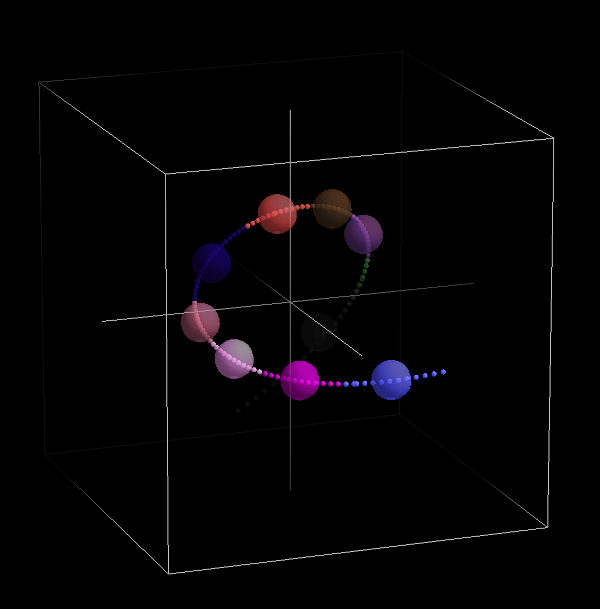
\includegraphics[width=0.6\textwidth]{logo.png} 
\end{center}
%%\\[1cm]

\tableofcontents

\newpage
\pagenumbering{arabic}
\pagestyle{scrheadings} 
%\pagestyle{scrplain} 
\clearscrheadfoot
%\rohead{\pagemark}
%\lohead{\headmark}
\ihead[\headmark]{\headmark}
\ohead[\pagemark]{\pagemark}

%%%%%%%%%%%%%%%%%%%%%%%%%%%%%%%%%%%%%%%%%%%%%%%%%%%%%%%%%%
\chapter{Introduction}



\verb+cost733class+ is a FORTRAN software package focused on creating and evaluating weather and 
circulation type classifications utilizing various different methods.
The name refers to COST Action 733 which has been an initiative started in the year 2005 within the ESSEM 
(Earth System Science and Environmental Management) domain of the COST (European Cooperation in 
Science and Technology) framework. The topic of COST 733 is "Harmonisation and Applications of Weather 
Type Classifications for European regions". \verb+cost733class+ is released under GNU General Public License v3 (GPL)
and freely available.



%%%%%%%%%%%%%%%%%%%%%%%%%%%%%%%%%%%%%%%%%%%%%%%%%%%%%%%%%%
\chapter{Installation}
The software is developed on Unix/Linux operating systems, however it may possible to compile and run it
on other operating systems too, although some features may not work. At the time of writing this affects 
the NetCDF and grib data format and the OpenGL visualization, which are not necessary to run the program.

%%%%%%%%%%%%%%%%%%%%%%%%%%%%%%%%%%%%%%%%%%%%%%%%%%%%%%%%%%
\section{Getting the source code}

When you read this, you might have downloaded the software package and unpacked it already. 
However here is the way how to get and compile the software:

To download direct your web browser to:
%\begin{verbatim}
\begin{lstlisting}
http://cost733class.geo.uni-augsburg.de/cost733class-1.2
\end{lstlisting}
%\end{verbatim}
Here you will find instructions how to download the source code by SVN or how to get a tar package.

If you have the tar-package unpack the bzip2 compressed tar-file e.g. by:
\begin{lstlisting}
tar xvfj cost733class-1.2_RC_revision??.tar.bz2
\end{lstlisting} where \verb+??+ stands for the svn version number.

Change into the new directory:
\begin{lstlisting}
cd cost733class-1.2
\end{lstlisting}

%%%%%%%%%%%%%%%%%%%%%%%%%%%%%%%%%%%%%%%%%%%%%%%%%%%%%%%%%%
\section{Using configure and make}

The next step is to compile the source code to generate the executable called \texttt{cost733class}. 
For this you need to have a C and a FORTRAN90 compiler installed on your system. 
The compiler reads the source code from the \verb+src+ directory and generates the executable \verb+src/cost733class+
in the same directory which can be started on the command line of a terminal. 
In order to prepare the compilation process for automatic execution, so called \verb+Makefile+s are generated by a script called \verb+configure+. 
The \verb+configure+ script checks whether everything (tools, libraries, compilers) which is needed for compilation is installed on your system. 
If \verb+configure+ stops with an error, you have to install the package it is 
claiming about (see troubleshooting) and rerun \verb+configure+ until it is happy and creates the \verb+Makefile+s.
The package include some example shell scripts containing the command to configure and make the software in one step:

\begin{itemize}
\item \verb!compile_gnu_debug.sh!: this script uses the GNU Linux compilers gcc, gfortran and c++ to compile the
software with NetCDF support but without GRIB and OpenGL support. Debugging information will be given in case of software errors.
\item \verb!compile_gnu_debug_opengl.sh!: this script additionally includes OpenGL support for visualization.
\item \verb!compile_gnu_debug_grib.sh!: this script additionally includes grib support.
\item \verb!compile_gnu_debug_omp.sh!:this script additionally includes compiler options to run parts of the code in parallel.
\item \verb!compile_intel_omp.sh!: this script uses the intel compiler suite.
\end{itemize}

In order to execute these scripts you type e.g.:
\begin{lstlisting}
./compile_gnu_debug_opengl.sh
\end{lstlisting}
or
\begin{lstlisting}
sh compile_gnu_debug_opengl.sh
\end{lstlisting}

These scripts can be easily copied and modified to save compiler options which are often needed. However it is also possible to run the two commands \verb!configure! and \verb!make! manually one after the other, as described in the following.

\subsection{configure}

The configure script tries to guess which compilers should be used, however
it is advisable to specify the compilers by setting the \verb+FC=+ and \verb+CC=+ flags. E.g. 
if you want to use the GNU compilers \verb+gfortran+ and \verb+gcc+ say:
\begin{lstlisting}
./configure FC=gfortran CC=gcc
\end{lstlisting}
or if the intel compilers should be used:
\begin{lstlisting}
./configure FC=ifort CC=icc
\end{lstlisting}
Note that the FORTRAN and C compilers should be able to work together, i.e. the binaries
must be compatible. This is not always the case e.g. when mixing other and GNU compilers (depending on versions).

Also you can use some special compiler options, e.g. for running parts of the classifications in parallel:
\begin{lstlisting}
./configure FC=ifort CC=icc FCFLAGS="-parallel -openmp"
\end{lstlisting}
In the same manner options for the C-compiler can be set by the \verb!CCFLAGS="..."! option.

By default \verb+cost733class+ compiles with netCDF, GRIB and OpenGL support.
Further options for the configure script control and disable special features of the package:
\begin{lstlisting}
./configure --disable-grib
\end{lstlisting}
switches off the compilation of the GRIB\_API, thus grib data can't be read by the software.
\begin{lstlisting}
./configure --disable-opengl
\end{lstlisting}
switches off the compilation of routines which visualize some of the classification processes like SOM, SAN or CKM.
This feature is working only for unix systems with opengl-development packages (gl-dev glut-dev x11-dev) installed.

\subsection{make}

The compiling process itself is done by the tool called \verb+make+:
\begin{lstlisting}
make
\end{lstlisting}

If everthing went well, you will find the executable \verb+cost733class+ in the src directory.
Check it by running the command:
\begin{lstlisting}
src/cost733class
\end{lstlisting}


If you have administrator privileges on your system you can install the executables into \verb+/usr/local/bin+.
Note that the NetCDF tools coming along with cost733class are also installed there.
\begin{lstlisting}
sudo su -
make install
\end{lstlisting}
Alternatively you can copy only the executable to any \verb+bin+ directory to have it in your
command search path:
\begin{lstlisting}
sudo copy src/cost733class /usr/local/bin
\end{lstlisting}

That's it, you can now start to run classifications, which of course needs some input data 
describing the atmospheric state of each time step (i.e. object) you want to classify. 
You can now try with the next chapter (Quick start) or look into the Data input chapter.


%%%%%%%%%%%%%%%%%%%%%%%%%%%%%%%%%%%%%%%%%%%%%%%%%%%%%%%%%%
\section{Manual compilation as an alternative}

Within the package directory there is a batch file called
\verb+compile_mingw.bat+ for Windows. This script file contains
the direct compile command for the \verb+gfortran+ and \verb+g95+ compiler without any 
dependencies to any libraries.
It can be used if no NetCDF input is needed or if there are troubles compiling
the NetCDF package.

%%%%%%%%%%%%%%%%%%%%%%%%%%%%%%%%%%%%%%%%%%%%%%%%%%%%%%%%%%
\section{Troubleshooting}

\subsection{For configure}
\begin{itemize}

\item If \verb+configure+ claims about something missing or a wrong version number, you have to
install or update the concerning software packages. 
For Debian and Ubuntu systems that's rather easy. 
First you have to find out the official name of the package which contains the files \verb+configure+ 
was claiming about. Here you can use the tool \verb+apt-file+ which must be installed first, updated and run: 
\begin{lstlisting}
sudo apt-get install apt-file
apt-file update
apt-file search <filename>
\end{lstlisting}
It will then print the name of the package in the first column and you can use it to install the missing package:
\begin{lstlisting}
sudo apt-get install <package>
\end{lstlisting}
\end{itemize}

\subsection{For make}
\begin{itemize}
 \item If the following error message appears:
\begin{lstlisting}
Catastrophic error: could not set locale "" to allow processing of 
multibyte characters
\end{lstlisting} 
setting the environment variable \verb+LANG+ to \verb+C+
\begin{lstlisting}
export LANG=C
\end{lstlisting} 
in the shell you use for compilation will fix it.
\end{itemize}

\subsection{For runtime problems}

\begin{itemize}
\item Some methods need a lot of RAM and maybe more than is available. If this is the case you can try 
to enlarge stack size each time you run the software by
\begin{lstlisting}
ulimit -s unlimited
\end{lstlisting}

\item If the following error or a similar error occurs:
\begin{lstlisting}
*** glibc detected *** double free or corruption (!prev): 0x08196948 ***
\end{lstlisting}
this is probably due to differing compiler/library versions. You can try to get rid of it by:
\begin{lstlisting}
export MALLOC_CHECK_=0
\end{lstlisting}
\item If compiled with grib support and running \verb+cost733class+ results in the following error:
\begin{lstlisting}
GRIB_API ERROR   :  Unable to find boot.def 
grib_context.c at line 156: assertion failure Assert(0)Aborted
\end{lstlisting}
one has to define the path to the so called grib definitions. In an Unix environment something like
\begin{lstlisting}
export GRIB_DEFINITION_PATH="/PATH/cost733class-1.2/grib_api-1.9.18/definitions"
\end{lstlisting}
should do it. Use absolute paths!

\item Depending on the processor type and data size method SAN and SOM may run for several hours up to days. This is no bug!
\end{itemize}
%%%%%%%%%%%%%%%%%%%%%%%%%%%%%%%%%%%%%%%%%%%%%%%%%%%%%%%%%%
\chapter{Getting started}

%%%%%%%%%%%%%%%%%%%%%%%%%%%%%%%%%%%%%%%%%%%%%%%%%%%%%%%%%%
\section{Principal usage}

\verb+cost733class+ has been written to simplify and unify the generation of classification catalogs.
It's functionality is controlled by command line arguments, i.e. options are given as key words after the command which is entered into a
terminal or console providing a command prompt. The command line interface (CLI) makes the software suitable for shell scripts and 
can easily run on compute servers or clusters in the background.
Recently a graphical user interface (GUI) has been added by using the OpenGL menu functions which is accessible by a right click into the 
OpenGL window, however it is not very intuitive yet. Therefore the documentation will concentrate on the CLI interface.


If you type \verb+src/cost733class+ just after the compilation process you will see the output of the \verb+-help+ function.
In order to run a classification, you have to provide command line arguments for the program, i.e. you have to
type expressions behind the \verb+cost733class+ command which are separated by blanks (" "). The program will scan
the command line and recognize all arguments beginning with a "-", several of which have to be followed by another expression.
All expressions have to be separated by one or more blanks, which is the reason that in between any expression (e.g. a file name) no blank is
allowed. Also all expressions have to be written in lower/upper case letters if said so in the \verb+-help+ output. 
Command lines can be rather simple, however some methods and the data configurations can be complex, 
thus that the command line gets longer and longer the more you want to fine tune your classification. 
In this case, and especially if just variations of a classifications should be run one after another, it can be useful to use shell 
scripts to run the software which will be explained below.

In order to understand which options play a role for which part of the classification it is helpful to distinguish between
options relevant for the data input and preprocessing and options relevant for the routines itself. 
In order to better understand how the software works and how it can be used, the workflow is briefly described in the following:

In the first step the command line arguments are analyzed (subroutine arguments()). For each option default values are set
within the program, however they are changed if respective options are provided by the user. 
The next step is to evaluate the data which should be read from a file, especially the size of the data set has to be determined here
in order to reserve (allocate) computer memory for it. Then the data are read into a preliminary array (RAWDAT) and eventually 
are preprocessed (selected, filtered, etc.) before they are put into the final, synchronized, DAT array which is used by the methods. In some cases 
(depending on the classification/evaluation operation) existing catalogs have to read. This is done in the next step by the subroutine classinput().
Afterwards the subroutine for the desired operation is called. If this subroutine finished with a new catalog, it is written to a classification
 catalogue file (*.cla) and the program ends. Other routines e.g. for comparison or evaluation of classification catalogs might just produce screen 
 output.

%%%%%%%%%%%%%%%%%%%%%%%%%%%%%%%%%%%%%%%%%%%%%%%%%%%%%%%%%%
\section{Quick start}
As an requirement to write complex commands it is necessary to understand the basic synopsis of \verb+cost733class+. There are several different use cases in which \verb+cost733class+ can be used:
\begin{enumerate}
  \item Creation of classifications of any numerical data following an entity-attribute-value model (main purpose of \verb+cost733class+). For more information about the data model used by \verb+cost733class+ see section \ref{datainput}.
  \item Evaluation of such classifications
  \item Comparison of such classifications
  \item Assignment of existing classifications to new data
  \item Rather simple data (pre)processing
\end{enumerate}
All of these use cases require different commands following different structures. Therefor the next sections give brief instructions on how to use \verb+cost733class+ for each of these five cases.

\subsection{Creating classifications}
For the creation of classifications a basic command follows the scheme:
\begin{lstlisting}
cost733class /*-dat/* <specification> [/*-dat/* <specification>] /*-met/* <method> [/*-ncl/* <integer>] [/*-cnt/* <filename>] [/*-cla/* <file>] [more method specific options]
\end{lstlisting}
Essential for a successful completion of each classification run is the \verb+-dat <specification>+ option which provides necessary information about the input data.
For some methods it is possible to give more than one data specification option, for others it is prerequisite. Furthermore the classification method must be named by the \verb+-met <method>+ option.
The number of classes can be specified with \verb+-ncl <integer>+. The filenames for the output of the classification catalog and the corresponding class centroids can be defined by 
\verb+-cla <filename>+ and \verb+-cnt <filename>+. Depending on the used classification method several other options can be provided by special options. For further documentation of these consult the relative section.\\
Based on this the command for a classification with the method KMN may look like:
\begin{lstlisting}
cost733class /*-dat/* /+pth:/+slp.dat /*-ncl/* 9 /*-met/* KMN /*-cla/* KMN_ncl9.cla
\end{lstlisting}

\subsection{Evaluating classifications}
The basic scheme of an evaluation command is:
\begin{lstlisting}
cost733class /*-dat/* <specification> [/*-dat/* <specification>] /*-clain/* <specification> /*-met/* <method> [/*-idx/* <filename>] [more method specific options]
\end{lstlisting}
The most important difference to a classification run is the \verb+-clain <specification>+ option.
It defines the path to an existing classification catalog file and is mandatory for all evaluation methods.
The desired evaluation method must be chosen by the \verb+-met <method>+ option. The results are written to one or more files for which the base name can be given by the \verb+-idx <filename>+ option.
Analogous to the previous command every method has its additional 
options which are explained in the corresponding sections below. At least one \verb+-dat <specification>+ option describes the data one wants to evaluate with.\\
A \verb+cost733class+ run which evaluates the classification generated 
by the previous command using the Brier Score would be:
\begin{lstlisting}
cost733class /*-dat/* /+pth:/+slp.dat /*-clain/* /+pth:/+KMN_ncl9.cla /*-met/* BRIER /*-idx/* brier_KMN_ncl9.txt
\end{lstlisting}

\subsection{Comparing classifications}
Comparing two or more classifications is rather easy:
\begin{lstlisting}
cost733class /*-clain/* <specification> [/*-clain/* <specification>] /*-met/* <method> [/*-idx/* <filename>] [more method specific options]
\end{lstlisting}
The only difference to an evaluation and classification run is the 
absence of the 
\verb+-dat <specification>+ option. Instead at least two 
classification catalogs (more than one per file are possible) must be provided.\\
A comparison of two partitions based on different methods could be 
done with:
\begin{lstlisting}
cost733class /*-clain/* /+pth:/+DKM_ncl9.cla /*-clain/* /+pth:/+KMN_ncl9.cla /*-met/* CPART /*-idx/* KMN_DKM_ncl9_compared.txt
\end{lstlisting}

\subsection{Assignment to existing classifications}
Assignments to existing classifications can be done on two different bases:
\begin{enumerate}
  \item for a given classification catalog
  \item for predefined class centroids
\end{enumerate}
In both cases one has to provide and describe data which is then assigned to an existing classification. Other required \verb+cost733class+ options differ in both cases. Please refer to the corresponding sections below.

\subsection{Rather simple (pre)processing}
Beyond the use cases mentioned above there are a few methods in \verb+cost733class+ which process input data in a different way. 
They are grouped together under the term miscellaneous functions.\\
Furthermore it is possible to just preprocess input data without calling a distinctive method.
\begin{lstlisting}
cost733class /*-dat/* <specification> [options for selecting dates] /*-writedat/* <filename>
\end{lstlisting}
In this case data output can be accomplished by the \verb+-witedat <filename>+ option. There are several flags for preprocessing and spatial selection which are listed and described in the relative section. An example might be:
\begin{lstlisting}
cost733class /*-dat/* /+pth:/+slp.dat /+lon:/+-10:30:2.5  /+lat:/+35:60:2.5 /+fdt:/+2000:1:1:12 /+ldt:/+2008:12:31:12 /+ddt:/+1d /+ano:/+3 /+fil:/+30 /*-per/* 2000:1:1:12,2005:12:31:12,1d /*-writedat/* output.bin
\end{lstlisting}
Note that here the output data are unformatted binary files (extension: bin). These files can be read by \verb+cost733class+ in a subsequent run. This proceeding can be very helpful if many runs of  \verb+cost733class+ are planned.

%%%%%%%%%%%%%%%%%%%%%%%%%%%%%%%%%%%%%%%%%%%%%%%%%%%%%%%%%%
\section{Help listing}

If you run the \verb+cost733class+ command without any command line argument (or with the \verb+-help+ option) 
you should see the following help text, giving a brief description of the various options:

\lstinputlisting{help.txt}

%\begin{scriptsize}
%%%\begin{verbatim}
%\verbatiminput{help.txt}
%%%\end{verbatim}
%\end{scriptsize}


%%%%%%%%%%%%%%%%%%%%%%%%%%%%%%%%%%%%%%%%%%%%%%%%%%%%%%%%%%
\chapter{Data input}
\label{datainput}
The first step of a \verb+cost733class+ run is to read input data. Depending on the use case these data can have very different formats. Principally there are two kinds: Foreign data
were not produced by \verb+cost733class+, whereas self-generated indeed are.

%%%%%%%%%%%%%%%%%%%%%%%%%%%%%%%%%%%%%%%%%%%%%%%%%%%%%%%%%%
\section{Foreign formats}
\label{fileformats}
\verb+cost733class+ can read any data in order to classify it. It is originally made for weather and
circulation type classification but most of the methods are able to classify anything, regardless of
the meaning of the data (only in some cases information about dates and spatial coordinates are necessary).
The concept of classification is to define \textit{groups}, \textit{classes} or \textit{types} (all these terms are used equivalently) encompassing \textit{objects}, \textit{entities}, \textit{cases} or \textit{objects} (again these terms mean more or less the same) belonging together. 
The rule how the grouping should be established differs from method to method, however in most of the cases the similarity between objects is utilized, while the definition of similarity differs again. In order to distinguish between various objects and to describe similarity or dissimilarity, each object is defined by a set of \textit{attributes} or \textit{variables} (this is what an entity is made of).
A useful model for the data representation is the concept of a rectangular matrix, where each row represents one object and each column represents one attribute of the objects. In case of ASCII-formatted input data this is exactly the way how the input data format is defined.

%%%%%%%%%%%%%%%%%%%%%%%%%%%%%%%%%%%%%%%%%%%%%%%%%%%%%%%%%%
\subsection{ASCII data file format}

ASCII text files have to be formatted in such a way that they contain the values of one object (time slice) in one line 
and the values for one variable (commonly a grid point) in a column. For more than one variable (grid point) the following columns
have to be separated by one or more blank letters (" "). Note that tabulator-characters (sometimes used by spread sheet programs as default) are not sufficient to separate columns! 
The file should contain a rectangular input matrix of numbers, 
i.e. constant number of columns at each row and a constant number of rows for each column. 
No missing values are allowed. 
The software evaluates an ASCII file 
on its own to find out the number of lines (days, objects, entities) and the number of variables 
(attributes, parameters, grid points). For this the numbers in one line have 
to be separated by one or more blanks (depending on the compiler commas or slashes may also
be used as separators between different numbers, but the comma never as decimal marker!!! 
The decimal marker must always be a point!). Thus you don't have to tell
how many lines and columns are in the file, but the number of columns has to be constant
throughout the file (the number of blanks between two attributes may vary though).
This format is fully compatible to the CSV (comma separated values) format which can be written
e.g. by spread sheet calculation programs. 
Note that no empty line is allowed. This can lead to read errors especially if there is
an empty line at the bottom of the file which is hard to see. 
If necessary, information about time and grid coordinates describing the data set additionally have to be provided within the
data set specification at the command line. In this case the ordering of rows and columns in the file must fit the following scheme: The first column is for the southernmost latitude 
and the westernmost longitude, the second column for the second longitude from west on the southernmost 
latitude, etc. The last column is for the easternmost and northernmost grid point. The rows represent the time steps.
All specifications have to fit to the number of rows and columns in the ASCII file.

%%%%%%%%%%%%%%%%%%%%%%%%%%%%%%%%%%%%%%%%%%%%%%%%%%%%%%%%%%
\subsection{COARDS NetCDF data format}

Cost733class includes the NetCDF library and is able to read 
NetCDF files directly and use the information stored in this self describing
data format. It has been developed using 6-hourly NCEP/NCAR reanalysis 
data \citep{Kalnay1996}, which are described and available at:
\url{http://www.cdc.noaa.gov/data/gridded/data.ncep.reanalysis.html} but also other
data sets following the COARDS conventions \\
(\verb+http://ferret.wrc.noaa.gov/noaa_coop/coop_cdf_profile.html+)
should be readable if they use the time unit of \verb+hours since 1-1-1 00:00:0.0+ or any other year.
In case of multi-file data sets the files have to be stored into one common directory and a running number
within the file names has to be indicated by \verb+?+ symbols, which are replaced by a running number given 
by the \verb+fdt:+ and \verb+ldt:+ flag (see below). 
Information about time and grid coordinates of the data set are retrieved from the 
NetCDF data file automatically. In case of errors resulting from buggy attributes of the time axis in NetCDF files try \verb+-readncdate+. Then the dates of observations are retrieved from the NetCDF time variable rather than calculating it from "actual range" attribute of the time variable.

%%%%%%%%%%%%%%%%%%%%%%%%%%%%%%%%%%%%%%%%%%%%%%%%%%%%%%%%%%
\subsection{GRIB data format}

Cost733class includes the GRIB\_API package and is able to read 
grib (version 1 \& 2) files directly and use the information stored in this self describing
data format. It has been developed using 6-hourly ECMWF 
data, which are described and available at:
\url{http://data-portal.ecmwf.int/data/d/interim_daily/} %but also other
%data sets following the COARDS conventions \\
%(\verb+http://ferret.wrc.noaa.gov/noaa_coop/coop_cdf_profile.html+)
%should be readable if they use the time unit of \verb+hours since 1-1-1 00:00:0.0+ or any other year.

In case of multi-file data sets the file paths have to contain running numbers
indicated by \verb+?+ symbols, or a combination of the following strings:
\verb+YYYY+ / \verb+YY+, \verb+MM+, \verb+DD+ / \verb+DDD+
; they are replaced by running numbers given 
by the \verb+fdt:+ and \verb+ldt:+ flags (see below). 
Information about time and grid coordinates of the data set are retrieved from the 
grid data file automatically.

%%%%%%%%%%%%%%%%%%%%%%%%%%%%%%%%%%%%%%%%%%%%%%%%%%%%%%%%%%
\subsection{Other data formats}
At the moment there is no direct support for other data formats.
Also it may be necessary to convert NetCDF-files first if e.g. the time axis is not
compatible.
A good choice in many aspects might be the software package CDO (climate data operators): \\
\verb+https://code.zmaw.de/projects/cdo+ which is released under GNU General Public License v2 (GPL).
Attention has to be paid to the type of calendar used. It can be adjusted by
\begin{lstlisting}
cdo setreftime,1-01-01,00:00,hours -setcalendar,standard input.nc output.nc
\end{lstlisting}
where \verb+hours+ has to be replaced e.g. by \verb+days+ or another appropriate 
time step if the time step given in the input file differs.

%%%%%%%%%%%%%%%%%%%%%%%%%%%%%%%%%%%%%%%%%%%%%%%%%%%%%%%%%%
\section{Self-generated formats}

%%%%%%%%%%%%%%%%%%%%%%%%%%%%%%%%%%%%%%%%%%%%%%%%%%%%%%%%%%
\subsection{Binary data format}
Binary data files are those written with \verb+form="unformatted"+ by FORTRAN programs. For input their structure
has to be known and provided by the specifications \verb+@lon:+, \verb+@lat:+, \verb+@fdt:+, \verb+@ldt:+ and eventually
\verb+@ddt:+ and \verb+@mdt+. Reading of unformatted data is considerably faster than reading formatted files. Therefore 
it might be a good idea to use the \verb+-writedat+ option to create a binary file from one or more other files if many 
runs of \verb+cost733class+ are planned. If the extension of the file name is \verb+*.bin+, unformatted files are assumed
by the program.

%%%%%%%%%%%%%%%%%%%%%%%%%%%%%%%%%%%%%%%%%%%%%%%%%%%%%%%%%%
\subsection{Catalog files}
\label{clainput}

For some procedures (like comparison, centroid calculation, assignment of data to existing catalogs, etc.) it is necessary
to read catalog files from disk. This is done using the option \verb+-clain <specification>+, where \verb+<specification>+ 
is similar to the specification of the data input option. The following specifications are recognized:
\begin{itemize}
\item  \verb+@pth:<file name>+
\item  \verb+@fdt:<first date>+
\item  \verb+@ldt:<last date>+
\item  \verb+@ddt:<time step, e.g. "@ddt:1d" for one day>+
\item  \verb+@dtc:<number of date columns>+
\item  \verb+@mdt:<list of months> e.g. @mdt:01,02,12+
\end{itemize}
See specifying data input for more details on these specifications. As with the data input, more than one classification catalog file 
may be used by providing more than one  \verb+-clain+ option. Note that all catalog files have to be specified with all necessary flags. Especially a wrong number of date columns could lead to errors in further steps.

\subsection{Files containing class centroids}
For the assignment to existing classifications it can be necessary to read files that contain class centroids. This is done with the \verb+-cntin <filename>+ option. Although there is support for NetCDF output of class centroids in 
\verb+cost733class+ at the time only ASCII files are supposed to be read successfully. A suitable file might be generated with the \verb+-cnt <filename>+ option in a previous run. The extension
of \verb+<filename>+ must be \verb+.dat+. For further information see section \ref{asc}.\\
Considering that such files can also be easily written with any text editor this feature of \verb+cost733class+ makes it possible to predefine class centroids or composites and assign data to them.

%%%%%%%%%%%%%%%%%%%%%%%%%%%%%%%%%%%%%%%%%%%%%%%%%%%%%%%%%%
\section{Specifying data input and preprocessing}

The data input and preprocessing steps are carried out in the following order:
\begin{itemize}
\item[1.] reading input data files (pth:)
\item[2.] grid point selection (slo: and sla:)
\item[3.] data scaling (scl:)
\item[4.] adding offset (off:)
\item[5.] centering/normalization of object (nrm:)
\item[6.] calculation of anomalies (ano:)
\item[7.] filtering (fil:)
\item[8.] area weighting  (arw:)
\item[9.] sequence construction (seq:)
\item[10.] date selection (options -dlist, -per, -mon, -hrs)
\item[11.] PCA of each parameter/data set separately (pca:, pcw:)
\item[12.] parameter weighting (wgt:)
\item[13.] overall PCA (options -pca, -pcw)
\end{itemize}

For reading data sets, the software first has to know how many variables (columns) and time steps (rows) are given in the files.
In case of ASCII files the software will find out these numbers by its own, if no description is given. 
However in this case no information about time and space is available and some functions will not work.
In case of NetCDF files this information is always given in the self describing file format. Thus the description of space and time
by specification flags on the command line can be omitted but will be available. 
Some methods like \verb+lit+ need to know about the date (provided e.g. by \verb+-per+, \verb+-mon+, etc.) of each object (e.g. day), 
or the coordinates (provided by \verb+@lon:+ and \verb+@lat:+) while other methods do not depend on it. If necessary the given dates
of a data set have to be described for each data set (or the first in case of same lengths) separately 
(see \verb+@fdt:+, \verb+@ldt:+ and \verb+@ddt:+ or \verb+@dtc:+). 

After the data set(s) is(are) loaded some selections and preprocessing can be done, again by giving specification 
flags (key words for only one single data set without a leading \verb+-+) and 
options (keywords which are applied to all data sets together with a leading \verb+-+).

%%%%%%%%%%%%%%%%%%%%%%%%%%%%%%%%%%%%%%%%%%%%%%%%%%%%%%%%%%
\subsection{Specification flags}

In order to read data from files which should be classified, these
data have to be specified by the \verb+-dat <specification>+ option.

It is important to distinguish between specification flags to describe the given data set as contained in the input files on the one hand and 
flags and options to select or preprocess these data.

The \verb+<specification>+ is a text string (or sequence of key words) providing all information
needed to read and process one data set (note that more data sets can be read, thus more than one specifications are needed). 
Each kind of information
within such a string (or key word sequence) is provided by a \verb+<flag>+ followed by a \verb+:+
and a \verb+<value>+. The different information sub strings have to follow the \verb+-dat+ option,
i.e. they are recognized to belong together to one data set as long as no other option beginning with
\verb+-+ appears. They may be concatenated by the \verb+@+ separator symbol directly together (without any blank ("\verb+ +") in between) 
or they may be separated by one or more blanks. The order of their appearance 
is not important, however if one flag is provided more than once, the last one will be used.
Please note that \verb+flags+ differ from \verb+options+ by the missing \verb+-+ (leading minus). 
The end of a specification of a data set is recognized by the occurrence of an option (i.e. by a leading \verb+-+).


The following flags are recognized:

%%%%%%%%%%%%%%%%%%%%%%%%%%%%%%%%%%%%%%%%%%%%%%%%%%%%%%%%%%
\subsection{Flags for data set description}
\begin{itemize}
\item \verb+var:<character>+ \\
        This is the Name of the variable. If the data are NetCDF
        files this must be exactly the variable name as in the
        NetCDF file, else it could not be found resulting in an
        error. If this flag is omitted the program tries to find the name on its own. 
        This name is also used to construct the file names
        for NCEP/NCAR Reanalysis data file (see the \verb+pth:+ flag).
        In case the format is ASCII the name is not important
        and this flag can be omitted, except for special methods based on
		special parameters (e.g. the wlk-method needs uwnd, vwnd, etc.).
        The complete \verb+var+ flag might look e.g. like: \verb+var:slp+
        
\item \verb+pth:<character>+ \\
        \begin{itemize}
        \item In case of ASCII format this is the path of the input file (its location directory including the file name). Please note that, depending on the system, some shortcuts for directories may not be recognized, like the ~ symbol for the home directory.
        E.g.: \verb+pth:/home/user/dat/slp.txt+.
        \item In case of a \verb+fmt:netcdf+ data set consisting of multiple subsequent files 
        the path can include \verb+?+ symbols
        to indicate that these letters should be replaced by a running number between
        the number given by \verb+fdt:+ and the number given by \verb+ldt: +.
        E.g. \verb+pth:/geo20raid/dat/ncep/slp.????.nc fdt:1948 ldt:2010+ (for a NetCDF multi-file data set).
        \item In case of \verb+fmt:grib+ the file name/path can include \verb+?+ symbols,
        or a combination of the following strings: \verb+YYYY+ / \verb+YY+, \verb+MM+, \verb+DD+ / \verb+DDD+
        ; to indicate that these letters should be replaced by a running number between
        the number given by \verb+fdt:+ and the number given by \verb+ldt:+,
        which has to have the same order and format as given in the path.
        E.g. \verb+pth:/data/YYYY/MM/slp.DD.grib fdt:2011:12:31 ldt:2012:01:01+ or \\
        \verb+pth:/data/slp.YYYY-MM-DD.grib fdt:2011:12:31 ldt:2012:01:01+ or \\
        \verb+pth:/data/slp.MMDDYYYY.grib fdt:12:31:2011 ldt:01:01:2012+ or \\
        \verb+pth:/data/slp.YYYY.grib fdt:2011:12:31 ldt:2012:01:01+ or \\
        \verb+pth:/data/slp.YYYYDDD.grib fdt:2011:001 ldt:2012:365+ \\
        (for grib multifile data sets).
        \end{itemize}

\item \verb+fmt:<character>+ \\
        This can be either ASCII, binary or NetCDF.
        \verb+ftm:ascii+ means the data are organized in text files:
        Each line holds one observation (usually the values of a day).
        Each column holds one parameter specifying the observations.
        Usually the columns represent grid points. These files have to
        hold a rectangular matrix of values, i.e. all lines have to
        have the same number of columns. Columns have to be separated
        by one or more blanks (" ") or by commas. Missing values are not allowed. 
        The decimal marker must be a point!\\
        \verb+fmt:netcdf+ means the data should be extracted from NetCDF files. If the 
        file name extension of the provided file name is \verb+.nc+ NetCDF format is assumed. 
        The information about data dimensions are extracted form the NetCDF files.
        \verb+fmt:binary+ denotes unformatted data. The dimensions of the data set have to provided 
        by the specifications \verb+@lon:+, \verb+@lat:+, \verb+@fdt:+, \verb+@ldt:+ and eventually
        \verb+@ddt:+ and \verb+@mdt+. This format is assumed if the file name extension is \verb+bin+.
        The default, which is assumed if no \verb+fmt:+ flag is given, is ASCII.

\item \verb+dtc:<integer>+ \\
        If the file format is \verb+fmt:ascii+ and there are leading columns
        specifying the date of each observation, this flags has to be used
        to specify how many date columns exist: "1" means that there is only
        one date column (the first column) holding the year, "2" means
        the two first columns hold the year and the month, "3" means the first
        three columns hold the year, the month and the day and "4" means the
        first four columns holds the year, month, day and hour of the observation.

\item \verb+fdt:YYYY:MM:DD:HH+ \\
		first date of data in data file (date for first line or row). Hours, days and months may be omitted.
		For data with \verb+fmt:netcdf+ in multiple files, it can be an integer number indicating the first year
		or running number which will be inserted to replace the \verb+?+ placeholder symbols in the file name.

\item \verb+ldt:YYYY:MM:DD:HH+ \\
		last date of data in data file (date for last line or row). Hours, days and months may be omitted.
		If so and \verb+ldt+ indicates a number of rows smaller than actually given in the file, only this smaller
		number of lines is used (omitting the rest of the file). For data with \verb+fmt:netcdf+ in multiple
		files, it can be an integer number indicating the last year
		or running number which will be inserted to replace the \verb+?+ placeholder symbols in the file name.

\item \verb+ddt:<int><y|m|d|h>+ \\
		time step of dates in data file in years, months, days or hours, e.g.: \verb+1d+ for daily data. 
		If \verb+ddt+ is omitted but both, \verb+fdt+ and \verb+ldt+ have same resolution it is automatically
		 set to one for that temporal resolution, e.g.: \verb+fdt:1850:01+ and \verb+ldt:2008:02+ and omitting
		  \verb+ddt+ will lead to \verb+ddt:1m+, i.e. monthly resolution. 
		
\item \verb+mdt:<list>+ \\
		list of months covered in data file, e.g. \verb+mdt:01:02:12+ if only winter data are given in the file. The list separator symbol may also be the comma "," instead of the ":".

\item \verb+lon:<number>:<number>:<number>+ \\
        This specifies the longitude dimensions of the input
        data as given in the file. The first \verb+<number>+ is the minimum longitude where
        longitudes west of 0 degree are given by negative numbers.
        The second \verb+<number>+ is the maximum longitude. The third
        \verb+<number>+ is the grid spacing in longitudes. 
        e.g.: \verb+lon:-30:50:2.5+
        This flag denotes just the description of the input data.
        For NetCDF data (which are self describing) it is superfluous!

\item \verb+lat:<number>:<number>:<number>+ \\
        This specifies the latitude dimensions of the input
        data. The first \verb+<number>+ is the minimum latitude where
        latitudes south of the equator are given by negative numbers.
        The second \verb+<number>+ is the maximum latitude. The third
        \verb+<number>+ is the grid spacing in latitudes. 
        e.g.: \verb+lat:30:70:2.5+
		Note that at the moment south-to-north order must be given in the 
		dat file, i.e. the left columns hold the southern-most latitudes.

\end{itemize}

%%%%%%%%%%%%%%%%%%%%%%%%%%%%%%%%%%%%%%%%%%%%%%%%%%%%%%%%%%
\subsection{Flags for spatial data Selection}

\begin{itemize}

\item \verb+slo:<number>:<number>:<number>+ \\
        If given, this flag selects a subset of grid points from the grid in the input data.
        The first \verb+<number>+ is the minimum longitude where
        longitudes west of 0 degree are given by negative numbers.
        The second \verb+<number>+ is the maximum longitude. The third
        \verb+<number>+ is the grid spacing in longitudes.
        The user must take care that the selected grid fits into the given grid!

\item \verb+sla:<number>:<number>:<number>+ \\
        If given, this flag selects a subset of grid points from the grid in the input data.
        The first \verb+<number>+ is the minimum latitude where
        latitudes south of the equator are given by negative numbers.
        The second \verb+<number>+ is the maximum latitude. The third
        \verb+<number>+ is the grid spacing in latitudes.
        The user must take care that the selected grid fits into the given grid!

%\item \verb+lev:<integer>+ \\
%        can describe levels for ascii service data format in the future

\item \verb+sle:<integer>+ \\
		This flag specifies the atmospheric level to be read
        if the \verb+fmt:ncepr+ flag is given. This is relevant for NetCDF data which may contain data of more than one level.
        If omitted the first level in the file is selected.

\end{itemize}
%%%%%%%%%%%%%%%%%%%%%%%%%%%%%%%%%%%%%%%%%%%%%%%%%%%%%%%%%%
\subsection{Flags for data Preprocessing}


\begin{itemize}
\item \verb+seq:<integer>+ \\
        This specifies whether this input data matrix should be
        extended in order to build sequences of observations for
        the classification. The \verb+<integer>+ specifies the length of
        the sequence. If this flag isn't provided then the sequence
        length is "1", i.e. no extension will be made. If it is "2" then
        one copy of the data matrix (shifted by one row/time step into the past) 
        will be concatenated to the right
        side of the original data matrix, resulting in a doubling of the
        variables (columns). This copy is shifted by 1 observation (line)
        downwards, thus each line holds the values of the original variable
        and the values of the preceding observation (e.g. day). In this
        way each observation is characterized additionally by the
        information of the preceding observation and the history of the
        variables are included for the classification. <integer> can be as
        high as desired, e.g. 12 for a sequence of 12 observations.
        In order to keep the original number of observations for the first
        lines (which do not have preceding observations) the values of
        the same observation are copied to fill up the gaps.

\item \verb+wgt:<number>+ \\
        If more than one data set is given each data set can be weighted
        relative to others, i.e. its values count more (or less) for
        determination of the similarity between the observations.
        If this flag is omitted the weight is 1.0 for all data and
        all data sets (each one defined by a \verb+-dat+ specification)
        are treated to have the same weight compared to each other by
        normalizing them separately as a whole (over space and time) 
        and multiplying them with a factor \verb+1/nvar+, where \verb+nvar+ is the 
        number of variables or attributes of each data set. 
		After that each data set is multiplied by the user weight \verb+<number>+. 

\item \verb+scl:<float>+ \\
		Scaling factor to apply to the input data of this parameter.

\item \verb+off:<float>+ \\
		Offset value which will be added to input data after scaling.

\item \verb+nrm:<integer>+ \\
		row-wise normalization: 
		1 = row-wise centralization of objects/patterns, 
		2 = row-wise normalization of objects/patterns (sample standard deviation), 
		3 = row-wise normalization of objects/patterns (population standard deviation)
		
\item \verb+ano:<integer>+, where integer can be 
\begin{itemize}
\item[-1]: column wise centralization of variables (grid points) after selection of time steps
\item[-2]: column wise normalization of variables using sample standard deviation (sum of squared deviations divided by n) after selection of time steps
\item[-3]: column-wise normalization of variables using population standard deviation (sum of squared deviations divided by n-1) after selection of time steps
\item[1]: column wise centralization of variables (grid points) before selection of time steps
\item[2]: column wise normalization of variables using sample standard deviation (sum of squared deviations divided by n) before selection of time steps
\item[3]: column-wise normalization of variables using population standard deviation (sum of squared deviations divided by n-1) before selection of time steps
\item[11] column-wise centralization of variables using the daily long-term mean for removing the annual cycle
\item[12] column-wise normalization of variables using the daily long-term mean and sample standard deviation for removing the annual cycle, 
\item[13]  column-wise normalization of variables using the daily long-term mean and population standard deviation for removing the annual cycle,
\item[21]  column-wise centralization of variables using the monthly long-term mean for removing the annual cycle, 
\item[22]  column-wise normalization of variables using the monthly long-term mean and sample standard deviation for removing the annual cycle, 
\item[23] column-wise normalization of variables using the monthly long-term mean and population standard deviation for removing the annual cycle,
\item[31] column-wise centralization of variables using the daily long-term mean of 31-day wide moving windows for removing the annual cycle
\item[32] column-wise normalization of variables using the daily long-term mean and sample standard deviation of 31-day wide moving windows for removing the annual cycle
\item[33]  column-wise normalization of variables using the daily long-term mean and population standard deviation of 31-day wide moving windows for removing the annual cycle
\end{itemize}

\item \verb+fil:<integer>+ \\        
		gaussian time filter of period <int>; int<0 = high-pass, int>0 = low-pass

\item \verb+arw:<integer>+ \\        
		Area weighting of input data grids: 0 = no (default), 1 = cos(latitude), 2 = sqrt(cos(latitude)), 3 = calculated weights by area of grid box which is the same as cos(latitude) of option 1.
        
\item \verb+pca:<integer|float>+ \\   		        
        parameter-wise pca:	If provided, this flag triggers a principal component analysis for compression of the input data. The PCA retains as many principal components as needed to explain at least a fraction of \verb+<real>+ of the total variance of the data or as determined by \verb+<integer>+. This can speed up the classification for large data sets considerably. Useful values are 0.99 or 0.95.
        
\item \verb+pcw:<integer|float>+ \\   		        
        parameter-wise pca with weighting of scores by explained variance: This preprocessing step works like \verb+pca+ but, weights the PCs according to their explained variance. This simulates the original data set in contrast to the unweighted PCs. In order to simulate the Euclidean distances calculated from the original input data (for methods depending on this similarity metric), the scores of each PC are weighted by sqrt(exvar(PC)) if \verb+-wgttyp euclid+ is set. Therefore if \verb+-pcw 1.D0+ is given (which actually doesn't lead to compression since as may PCs as original variables are used) exactly the same euclidean distances (relative to each other) are calculated.

\end{itemize}        
%%%%%%%%%%%%%%%%%%%%%%%%%%%%%%%%%%%%%%%%%%%%%%%%%%%%%%%%%%
\subsection{Flags for data post processing}
\begin{itemize}  

\item \verb+cnt:<file>.<ext>+ \\
		write parameter composite (centroid) to file of format depending on extension: 
		.txt = ascii-xyz data, .nc = netcdf, 
		%.ctl = grads data, .grs = grass-gis raster file, .grd = surfer ascii grid, .svc = service format

\end{itemize}

%%%%%%%%%%%%%%%%%%%%%%%%%%%%%%%%%%%%%%%%%%%%%%%%%%%%%%%%%%
\subsection{Options for selecting dates}

If there is at least one input data set with given flags for date description, this 
information about the time dimension can be used to select dates or time steps for the 
procedure. Such a selection applies to all data sets if more than one is used.

Note that the following switches are options beginning by a \verb+-+ because they apply to 
the whole of the data set:
\begin{itemize}

\item \verb+-per YYYY:MM:DD:HH,YYYY:MM:DD:HH,nX+ \\
		This option selects a certain time period, starting at
		a certain year (1st YYYY), month (1st MM), day (1st DD) and hour (1st HH),
		ending at another year (2nd YYYY), month (2nd MM), day (2nd DD) and hour (2nd HH),
		and stepping by n time units (nX). The stepping information can be omitted. Time unit X can be:
		\begin{itemize}
		\item \verb+y+ for years
		\item \verb+m+ for months
		\item \verb+d+ for days
		\item \verb+h+ for hours. Stepping for hours must be 12, 6, 3, 2 or 1
		\end{itemize}
		The default stepping is 1 while the time unit for the stepping (if omitted) is assumed 
		to be the last date description value (years if only is given YYYY, months if also MM is provided, days for DD or hours for HH).

\item \verb+-mon 1,2,3+ \\
		In combination with the \verb+-per+ argument the number of months used by the software can be restricted by the 
		\verb+-mon+ option followed by a list of month numbers. 

\item \verb+-dlist <file>+ \\
		Alternatively it is possible to select time steps (continuously or discontinuously) 
		and for both NetCDF and ASCII data by the \verb+-dlist <file>+ option.
		The given file should hold as many lines as time steps should be selected and
		four columns for the year, month, day and hour of the time step. These
		numbers should be integer and separated by at least one blank.
		Even if no hours are needed they must be given as a dummy.
\end{itemize}

Note that it is possible to work with no (or fake) dates, allowing for input of ASCII-data sets 
which have been selected by another software before.


%%%%%%%%%%%%%%%%%%%%%%%%%%%%%%%%%%%%%%%%%%%%%%%%%%%%%%%%%%
\subsection{Using more than one data set}

More than one data set can be used by just giving more than one
\verb+-dat <specification>+ option (explained above) within the command line. 
The data of a second (or further) data set are then pasted behind the data of the first 
(or previous) data set as additional variables (e.g. grid points or data matrix 
columns) thus defining each object (e.g. day or data matrix rows) additionally.
Note that these data sets must have the same number of objects (lines or records) in order 
to fit together.

If one of the data sets is given in different physical units than the others (e.g. hPa and Kelvin), 
there must be taken care of the effect of this discrepancy for the distance metric used for 
classification.

\begin{enumerate}
\item For all metrics the data set with higher total variance (larger numbers) will have larger influence.
\item For correlation based metrics, if there is a considerable difference of the mean between two data sets, 
this jump can result in strange effects. E.g. for t-mode PCA (PPT) there might be just one single class explaining this jump
while all other classes are empty. 
\end{enumerate}

Therefore in case of using more than one data set (i.e. multi-field classification) each data set 
(separately from the others) should be normalized as a whole (one single mean and standard deviation 
for all columns and rows of this single data set together). This can be achieved by using the flag
\begin{itemize}
\item \verb+@wgt:<float>+
\end{itemize}
at least for one data set. Where \verb+<float>+ can be \verb+1.D0+ (the \verb+D+ is for double precision) 
in order to apply a weight of $1.0$.

If a weighting factor is given using the flag \verb+wgt:<float>+, 
the normalized data sets are multiplied with this factor respectively. 
The default value is $1.D0$, however it will be applied only if at least for one data set the flag
\verb+@wgt:<float>+ is given! If this is the case, always all data sets will be normalized and weighted
(eventually with $1.D0$ if no individual weight is given).

In case of methods using the Euclidean distance 
the square root of the weight is used in order to account for the square in the distance 
calculations. This allows for a correct weight of the data set in the distance measure. 
Also different numbers of variables (grid points) are accounted for by dividing the data by 
the number of variables. Therefore the weight is applied to each data set as a whole in respect 
to the others.
If e.g. a weight of 1.0 is given to data set A (\verb+wgt:1.0+) and a weight of 0.5 is given to 
data set B (\verb+wgt:0.5+) then data set A has a doubled influence on the assignment of objects 
to a type compared to data set B, regardless how many variables (grid points) data set A or B has 
and regardless what the units of the data has been.

It is advisable always to specify the \verb+wgt:<float>+ flag for all data sets if multiple data 
sets are used. E.g.

\begin{lstlisting}
cost733class /*-dat/* /+pth:/+slp.txt /+wgt:/+1.D0 /*-dat/* /+pth:/+shum.txt /+wgt:/+1.D0 /*-met/* XYZ
\end{lstlisting}

%%%%%%%%%%%%%%%%%%%%%%%%%%%%%%%%%%%%%%%%%%%%%%%%%%%%%%%%%%
\subsection{Options for overall PCA preprocessing of all data sets together}
Apart from the possibility to apply Principal Component Analysis to each parameter data set separately,
 the option \verb+-pca <float|integer>+ allows a final PCA of the whole data set. As with the separate
 procedure the number of PC's to retain can be given as an integer number or, in case of a floating number,
 the fraction of explained variance to retain can be specified. Also automatic weighting of each PC with it's fraction of explained variance can be obtained by using the \verb+-pcw <float|int>+ flag instead of \verb+-pca+.

%%%%%%%%%%%%%%%%%%%%%%%%%%%%%%%%%%%%%%%%%%%%%%%%%%%%%%%%%%
\section{Examples}


\subsection{Simple ASCII data matrix}

\begin{lstlisting}
cost733class /*-dat/* /+pth:/+era40_MSLP.dat /+fmt:/+ascii /+lon:/+-37:56:3 /+lat:/+30:76:2 /*-met/* kmeans /*-ncl/* 9
\end{lstlisting}
This will classify data from an ASCII file \verb+(era40_MSLP.dat)+ which holds as many columns as
given by the grid of -37 to 56 degree longitude (3 degree spacing) and 30 to 76 degree latitude
(2 degree spacing). Thus the file has \verb+(56-(-37))/3+1 by (76-30)/2+1 columns (=32x24=768).
The ordering of the columns follows the principle: longitudes vary fastest from west to east,
latitudes vary slowest from south to north. Thus the first column is for the southernmost latitude 
and the westernmost longitude, the second column for the second longitude from west on the southernmost 
latitude, etc. The last column is for the easternmost and northernmost grid point as illustrated in table \ref{asciidatamatrix}
\begin{table}
\label{asciidatamatrix} 
\begin{scriptsize}
\begin{tabular}{|c|c|c|c|c|c|c|c|}
\hline 
  \verb+ +   & \verb+colum #1+          & \verb+column #2+         &     & \verb+column #32+       & \verb+column #33+        &     & \verb+column #768+ \\ 
  \verb+ +   & \verb+lon=-37,lat=30+    & \verb+lon=-34,lat=30+    & ... & \verb+lon=56,lat=30+    & \verb+lon=-37,lat=32+    & ... & \verb+lon=56,lat=76+ \\ 
\hline 
  \verb+t=1+ &  \verb+mslp(-37,30,1)+    &  \verb+mslp(-34,30,1)+    & ... & \verb+mslp(56,30,1)+    &  \verb+mslp(-37,32,1)+    & ... &   \verb+mslp(56,76,1)+ \\
\hline 
  \verb+t=2+ &  \verb+mslp(-37,30,2)+    &  \verb+mslp(-34,30,2)+    & ... & \verb+mslp(56,30,2)+    &  \verb+mslp(-37,32,2)+    & ... &   \verb+mslp(56,76,2)+ \\
\hline
  \verb+...+  &      \verb+...+         &    \verb+...+            & ... &  \verb+...+             &    \verb+...+            & ... &    \verb+...+          \\
\hline
  \verb+t=nt+ & \verb+mslp(-37,30,nt)+    &  \verb+mslp(-34,30,nt)+    & ... & \verb+mslp(56,30,nt)+    &  \verb+mslp(-37,32,nt)+    & ... &   \verb+mslp(56,76,nt)+ \\
\hline
\end{tabular} 
\end{scriptsize}
\caption{Example data matrix of mean sea level pressure values formatted to hold grid points in columns varying by $lon=-37,56$  by  $3^\circ$ and by $lat=30,76$  by  $2^\circ$ and time steps $t=1,nt$ in rows.}
\end{table}
Note that the command line could have been written as
\begin{lstlisting}
cost733class /*-dat/* /+pth:/+era40_MSLP.dat /+lon:/+-37:56:3 /+lat:/+30:76:2 /*-met/* kmeans /*-ncl/* 9
\end{lstlisting}
to achieve exactly the same result. All flags are recognized to belong to the \verb+-dat+ option until another
option beginning with \verb+-+ appears.
Note that in this example no information about the time was made, i.e. the date of each line is unknown to the program.
In this case this is unproblematic because k-means doesn't care about the meaning of objects, it just classifies it 
according to their attributes (the pressure values at the grid points in this case).

\subsection{ASCII data file with date columns}
\begin{lstlisting}
cost733class /*-dat/* /+pth:/+station/zugspitze_2000-2008_Tmean.dat /+dtc:/+3 /+ano:/+33 /*-met/* BIN /*-ncl/* 10
\end{lstlisting}
In this example the software is told, that there are three leading columns in the file holding the date of each line
(year, month, day because there are 3 columns and this is the hierarchy per definition, there is no way to change this order).
The total number of columns (four) and the number of rows is detected by the software itself by counting the blank-gaps in the lines.
The beginning of this file looks like shown in table \ref{asciidatadate}
\begin{table}
\label{asciidatadate} 
\begin{scriptsize}
\begin{tabular}{|c|c|c|c|}
\hline 2000 & 01 & 01 & -12.1 \\
\hline 2000 & 01 & 02 & -10.3 \\
\hline 2000 & 01 & 03 & -6 \\
\hline 2000 & 01 & 04 & -7.3 \\
\hline 2000 & 01 & 05 & -7.7 \\
\hline 2000 & 01 & 06 & -6.6 \\
\hline 2000 & 01 & 07 & -8 \\
\hline 2000 & 01 & 08 & -9.1 \\
\hline 2000 & 01 & 09 & -10.3 \\
\hline 2000 & 01 & 10 & -11.1 \\
\hline 2000 & 01 & 11 & -12 \\
\hline 2000 & 01 & 12 & -8.7\\
\hline 2000 & 01 & 13 & -11.2 \\
\hline 2000 & 01 & 14 & -9.6 \\
\hline ... & ... & ... & ... \\
\hline 2008 & 12 & 31 & -8 \\
\hline 
\end{tabular} 
\end{scriptsize}
\caption{Example ASCII file contents including three date columns for year, month and day.}
\end{table}
Also there is an option \verb+ano:33+ in order to use the anomalies (deviation) referring to the long-term daily mean.
Afterwards the method \verb+BIN+ is called which by default just calculates equally spaced percentile thresholds to define
10 (\verb+-ncl 10+) classes, to which the data is assigned. Note that this method uses only the first column (after any date columns of course).


\subsection{NetCDF data selection}
\begin{lstlisting}
cost733class /*-dat/* /+var:/+hgt /+pth:/+/data/20thC_ReanV2/hgt.????.nc /+fdt:/+1871 /+ldt:/+2008 /+slo:/+-50:50:2.0 /+sla:/+20:50:2.0 /+sle:/+0950 /*-writedat/* hgt_0950_slo-50-50_sla-20-50_1871-2008.bin
\end{lstlisting}
This command selects a sub grid from 50\degree west to 50\degree east by 2\degree and from 20\degree north to 50\degree north (by 2\degree)
out of the global reanalysis (\verb+20thC_ReanV2+) grid. After input in this case the data are written to a binary file, which can be used for further 
classification by subsequent runs. But of course it would have been possible to provide a \verb+-met+ option to start a classification in this run.
Note that this call needs 1.2 GB of memory.

\subsection{Date selection for classification and centroids}
\begin{lstlisting}

cost733class /*-dat/* /+pth:/+grid/slp.dat /+lon:/+-10:30:2.5 /+lat:/+35:60:2.5 /+fdt:/+2000:1:1 /+ldt:/+2008:12:31 /+ddt:/+1d /*-met/* CKM /*-ncl/* 8 /*-per/* 2000:1:1,2008:12:31,1d /*-mon/* 6,7,8 /*-v/* 3

cost733class /*-dat/* /+pth:/+grid/slp.dat /+lon:/+-10:30:2.5 /+lat:/+35:60:2.5 /+fdt:/+2000:1:1 /+ldt:/+2008:12:31 /+ddt:/+1d /+cnt:/+DOM00.nc /*-clain/* /+pth:/+CKM08.cla /+dtc:/+3 /+fdt:/+2000:6:1 /+ldt:/+2008:8:31 /+mdt:/+6:7:8 /*-per/* 2000:1:1,2008:12:31,1d /*-mon/* 6,7,8 /*-met/* CNT /*-v/* 3
\end{lstlisting}
Here classification is done only for summer months (\texttt{-per 2000:1:1,2008:12:31,1d -mon 6,7,8}) and written to 
\verb+CKM08.cla+ in the first run. In the second call \verb+CKM08.cla+ is used to build centroids, again only for the summer months.
Note that \verb+mdt:6:7:8+ has to be provided for the \verb+-clain+ option in order to read the catalog correctly.

%%%%%%%%%%%%%%%%%%%%%%%%%%%%%%%%%%%%%%%%%%%%%%%%%%%%%%%%%%
\chapter{Data output}

%%%%%%%%%%%%%%%%%%%%%%%%%%%%%%%%%%%%%%%%%%%%%%%%%%%%%%%%%%
\section{The classification catalog}
This is a file containing the list of resulting class numbers. Each line represents one
classified entity. If date information on
the input data was provided the switch \verb+-dcol <int>+  can be used
to write the datum to the classification output file
as additional columns left to the class number. The argument
\verb+<int>+ decides on the number of date columns:
\verb+-dcol 1+ means only one column for the year or running number in case of fake dates (1i4), \verb+-dcol 2+
means year and month (1i4,1i3), \verb+-dcol 3+
means year, month and day (1i4,2i3) and \verb+-dcol 4+ means year,
month, day and hour (1i4,3i3). If the \verb+-dcol+ option is missing the routine tries to guess 
the best number of date columns. This number might be important if the catalog file is used in subsequent 
runs of cost733class e.g. for evaluation etc.

%%%%%%%%%%%%%%%%%%%%%%%%%%%%%%%%%%%%%%%%%%%%%%%%%%%%%%%%%%
\section{Centroids or type composites}

If the \verb+-cnt <filename>+ option is given, a file is created which contains the data of the
centroids or class means. In each column of the file the data of each class is written. Each line/row of the file 
corresponds to the variables in the order (of the columns) provided in the input data.\\
If the \verb+cnt:<file.nc>+ flag has been given within the individual specification of a data set,
the corresponding centroids for this parameter will be written to an extra file. Thus it is possible to 
easily discern the type composites for different parameters. The file format depends on the extension of the 
offered file name: the file name extension ".nc" leads to NetCDF output (which might be used for plotting with grads), 
the file name extension ".txt" denotes ASCII output including grid point coordinates in the first two columns if available,
while the extension "dat" skips the coordinates in any case (useful for viewing or for further processing e.g. with \verb+-met asc+).

%In case one of the following flags have been
%given within the data set specifications, the centroids for this parameters
%are written into extra files of the respective file format:
%\begin{itemize}
%\item \verb+ctxt:<filename>+: xyz-text file
%\item \verb+cctl:<filename>+: grads binary grid control and data file
%\item \verb+cgrs:<filename>+: grass-gis raster file (read into EPSG 4326 location)
%\item \verb+cgrd:<filename>+: surfer ascii grid file
%\end{itemize}

%%%%%%%%%%%%%%%%%%%%%%%%%%%%%%%%%%%%%%%%%%%%%%%%%%%%%%%%%%
\section{Output on the screen}
The verbosity of screen output can be controlled by the \verb+-v <int>+ flag. <int> can be:
\begin{itemize}
\item[0]: NONE: errors only
\item[1]: MAIN: warnings, major calls and proceeding
\item[2]: SUB: major subroutine's calls and proceeding, routine's major results
\item[3]: DET: detailed/all calls/proceeding, routine's intermediate results (no arrays)
\item[4]: ALL: extensive results (arrays etc.)
\end{itemize}

At the end of each classification the explained cluster variance (ECV) is calculated and printed on the screen.


Further on the final class frequencies are printed on the screen.

%%%%%%%%%%%%%%%%%%%%%%%%%%%%%%%%%%%%%%%%%%%%%%%%%%%%%%%%%%
\section{Output of the input data}
Providing the option \verb+-writedat <filename>+ writes the input data to a single file as it would be used for 
classification, i.e. after application of the preprocessing steps if any. The type of the resulting file depends on its extension. \verb+.bin+ causes unformatted binary output whereas any other extension produces simple ASCII output.  Note that this function can be used to 
prepare and compile data sets which can be used for input into \verb+cost733class+ or any other software later.
Thus if no method is specified \verb+cost733class+ can be used as a pure data processing tool.

%%%%%%%%%%%%%%%%%%%%%%%%%%%%%%%%%%%%%%%%%%%%%%%%%%%%%%%%%%
\section{Output of indices used for classification}
Some methods are based on indices which are calculated as intermediate results (e.g. PCA methods calculate scores or loadings time series).
The flag \verb+-idx <filename>+ causes those methods to write out these indices into the according file.
%%%%%%%%%%%%%%%%%%%%%%%%%%%%%%%%%%%%%%%%%%%%%%%%%%%%%%%%%%
\section{Opengl graphics output}
If compiled with opengl support (./configure --enable-opengl) the switch -opengl opens a x11-window
for visualization of the classification process for some optimization methods. Additionally
the switch -gljpeg produces single image files for each frame which can be used to produce an animation, 
eg. by using the unix command:
\begin{lstlisting}
ffmpeg -y -r 20 -sameq -i out\%06d.jpg -vcodec mjpeg -f avi cost733ckm.avi
\end{lstlisting}

%%%%%%%%%%%%%%%%%%%%%%%%%%%%%%%%%%%%%%%%%%%%%%%%%%%%%%%%%%
\chapter{Classification methods}

%%%%%%%%%%%%%%%%%%%%%%%%%%%%%%%%%%%%%%%%%%%%%%%%%%%%%%%%%%%%%%%%%%%%%%%%
%\section{Basic notes on distance metrics}
%\label{distfuncs}
%In \verb+cost733class+ many methods, especially the classification algorithms, make use of so called distance metrics. They are more or less a measure of similarity between two objects with the same number of attributes. \\

\section{Methods using predefined types}

\subsection{INT | interval | BIN | binclass}

This method classifies the objects into bins which are defined either by
thresholds calculated as the fraction of the range of a variable or
by percentiles of the variable distribution.

\subsubsection*{Options}
Strictly necessary options:
\begin{itemize}
 \item \verb+-dat <specification>+:\\ Input data. No grid description is necessary.
\end{itemize}
The following options define the classification:
\begin{itemize}
 \item \verb+-ncl <int>+:\\ Determine the number of classes/bins. Default is 9.
 \item \verb+-svar <int>+:\\ The variable/column number of the input data set which should be used to calculate the bin thresholds. Default is 1.
 \item \verb+-crit <int>+:\\ Determine the threshold type, where \verb+<int>+ may be:
 \begin{itemize}
 \item[1]: Means the threshold is the i'th percentile where, i is cl*1/ncl.
 \item[2]: Means the ncl bins are centered around the mean value and have the size of the dev*2/ncl, where dev is the largest deviation from the mean within data set.
 \item[3]: Means the bin size is the data range divided by ncl, the bins are not centered.
 \item[4]: Classification into 2 bins: a lower of values less than \verb+-thres <real>+ for \verb+-svar <int>+ and one above.
 \item[5]: As in \verb+-crit 4+: but the threshold is interpreted as a percentile threshold between 0 and 100\%. 
 \end{itemize}
 \item \verb+-dist 0+:\\ For \verb+-crit 1+ and \verb+-crit 5+ the percentiles are calculated without the minimum value of var. This is useful e.g. for daily 
precipitation with 
many dry days. 
\end{itemize}
Options for data output:
\begin{itemize}
 \item \verb+-cla <filename>+:\\ Output file name for the classification catalog.
 \item \verb+-dcol <int>+:\\ Number of date columns in the classification catalog.
 \item \verb+-cnt <filename>+:\\ Output file name for the class centroids.
\end{itemize}

\subsubsection*{Output}
This method returns one file containing the classification catalog. 
Overall class centroids and centroids for each input data set are optional.

\subsubsection*{Examples}
An example with default values:
\begin{lstlisting}
cost733class /*-dat/* /+pth:/+slp.????.nc /+fmt:/+netcdf /+fdt:/+1951 /+ldt:/+1980 /--met/- INT /--ncl/- 9 /--crit/- 1 /--svar/- 1 /*-cla/* INT.cla /*-dcol/* 4 
\end{lstlisting}
Another example:
\begin{lstlisting}
cost733class /*-dat/* /+pth:/+slp.????.nc /+fmt:/+netcdf /+fdt:/+1951 /+ldt:/+1980 /--met/- INT /--ncl/- 20 /--crit/- 2 /*-cnt/* INT.cnt /*-cla/* INT.cla /*-dcol/* 4 
\end{lstlisting}
This run classifies the input data into 20 bins and writes a classification catalog and centroid file.

%%%%%%%%%%%%%%%%%%%%%%%%%%%%%%%%%%%%%%%%%%%%%%%%%%%%%%%%%%%%%%%%%%%%%%%%
\subsection{GWT | prototype - large scale circulation types}
\label{met:GWT}

This method uses three prototype patterns and calculates the three Pearson correlation coefficients between
each field in the input data set and the three prototypes \citep{Beck2007}. The first prototype is a strict zonal pattern with 
values increasing from north to south. The second is a strict meridional pattern with values increasing from west
to east. And the third is a cyclonic pattern with a minimum in the center and increasing values to the margin 
of the field. Depending on the three correlation coefficients and their combination each input field is 
classified to one class.
Since there are only fixed numbers of combinations, not all numbers of types can be achieved.
This method makes sense only for single pressure fields. The possible numbers of types are: 8, 10, 11, 16, 18, 19, 24, 26, 27.
For 8 types the main wind sectors (N, NE, E, SE, S, SW, W, NW) are used. Two additional types for pure cyclonic and pure 
anticyclonic situations lead to 10 types and an indifferent type according to cyclonicity to 11 types.
For 16 types the following numbers apply: 1-8=cyclonic, 9-16=anticyclonic 
and for 24:  1-8=cyclonic, 9-16=anticyclonic, 17-24=indifferent. Adding 2 or 3 cyclonicity types then results in
18 or 19 and 26 or 27 types accordingly.

\subsubsection*{Options}
Strictly necessary options:
\begin{itemize}
 \item \verb+-dat <specification>+:\\ Input data. Grid description is necessary!
\end{itemize}
The following options define the classification:
\begin{itemize}
 \item \verb+-ncl <int>+:\\ The number of types as described above. Default is 8.
 \item \verb+-crit <int>+:\\ Vorticity index. \verb+<int>+ can be:
 \begin{itemize}
 \item \verb+1+: No normalization of the vorticity index.
 \item \verb+2+: Normalization of the vorticity index.
 \end{itemize}
\end{itemize}
Options for data output:
\begin{itemize}
 \item \verb+-cla <filename>+:\\ Output file name for the classification catalog.
 \item \verb+-dcol <int>+:\\ Number of date columns in the classification catalog.
 \item \verb+-idx <basename>+:\\ Output base name for pattern correlations.
 \item \verb+-cnt <filename>+:\\ Output file name for the class centroids.
\end{itemize}

\subsubsection*{Output}
This method returns one file containing the classification catalog. The three prototype patterns are written to NetCDF files (\verb+proto001.nc+ to \verb+proto003.nc+) in the directory where \verb+cost733class+ was executed (only for \verb+-v 4+ and higher).
Overall class centroids as well as a file containing the pattern correlations at each time step are optional.

\subsubsection*{Examples}
An example with default values:
\begin{lstlisting}
cost733class /*-dat/* /+pth:/+slp.dat /+fmt:/+ascii /+lon:/+-37:56:3 /+lat:/+30:76:2 /--met/- GWT /--ncl/- 8 /--crit/- 1 /*-cla/* GWT09.cla /*-dcol/* 3 
\end{lstlisting}
Another example:
\begin{lstlisting}
cost733class /*-dat/* /+pth:/+slp.dat /+fmt:/+ascii /+lon:/+-37:56:3 /+lat:/+30:76:2 /--met/- GWT /--ncl/- 27 /--crit/- 2 /*-cla/* GWT27.cla /*-dcol/* 3 
\end{lstlisting}


%%%%%%%%%%%%%%%%%%%%%%%%%%%%%%%%%%%%%%%%%%%%%%%%%%%%%%%%%%%%%%%%%%%%%%%%
\subsection{GWTWS | gwtws - large scale circulation types}

Based on GWT (Cap. \ref{met:GWT}). The classification is done using GWT with 8 types for the 500mb geopotential.
If the mean wind speed at 500mb (derived from the geopotential field) is lower than 7m/s, it's "convective", resulting in one of the following three types:
\begin{itemize}
\item if the mean sea level pressure is lower than 1010mb it's "low" (type 9)
\item if the mean sea level pressure is higher than 1015mb it's "high" (type 10)
\item else or if the mean wind speed at 500mb is lower than 3m/s it's "flat" (type 11)
\end{itemize}
If the mean wind speed at 500mb is higher than 7m/s, it's "advective", and the types are identical to GWT using 8 types.

\subsubsection*{Options}
Strictly necessary options:
\begin{enumerate}
 \item \verb+-dat <specification>+:\\ Input data, the 500mb geopotential field. Grid description is necessary!
 \item \verb+-dat <specification>+:\\ Input data, the sea level pressure, as field or mean value. Grid description is necessary!
\end{enumerate}
The following options define the classification:
\begin{itemize}
 \item \verb+-crit <int>+:\\ Handling of thresholds. \verb+<int>+ can be:
 \begin{itemize}
 \item[1]: the four thresholds (default: 7m/s, 3m/s, 1010mb and 1015mb) can be varied in the following matter:
 \begin{itemize}
  \item a mean windspeed at 500mb lower than \texttt{-alpha <real>} [m/s] will result in one of the following three types:
  \item if the mean sea level pressure is lower than \texttt{-gamma <real>} [mb] it's "low" (type 9)
  \item if the mean sea level pressure is higher than \texttt{-delta <real>} [mb] it's "high" (type 10)
  \item if the mean windspeed at 500mb is lower than \texttt{-beta <real>} [m/s] it's "flat" (type 11)
 \end{itemize}
 \item[2]: the four thresholds (default: 0.275, 0.073, 0.153 and 0.377) can be varied half-automatized as the values for mean wind speed at 500mb and mean sea level pressure rise or descend a given percentile (alpha, beta, gamma or delta [0,1]):
\begin{itemize}
\item a mean windspeed at 500mb lower than \texttt{-alpha <real>} will result in one of the following three types:
\item if the mean sea level pressure is lower than \texttt{-gamma <real>} it's "low" (type 9)
\item if the mean sea level pressure is higher than \texttt{-delta <real>} it's "high" (type 10)
\item if the mean windspeed at 500mb is lower than \texttt{-beta <real>} it's "flat" (type 11)
\end{itemize}
 \end{itemize}
\end{itemize}
Options for data output:
\begin{itemize}
 \item \verb+-cla <filename>+:\\ Output file name for the classification catalog.
 \item \verb+-idx <basename>+:\\ Output base name for means of MSLP and wind speed at 500mb per time step.
 \item \verb+-dcol <int>+:\\ Number of date columns in both files mentioned above.
 \item \verb+-cnt <filename>+:\\ Output file name for the class centroids.
\end{itemize}

\subsubsection*{Output}
This method returns one file containing the classification catalog. The three prototype patterns are written to NetCDF files (\verb+proto001.nc+ to \verb+proto003.nc+) in the directory where \verb+cost733class+ was executed.
Parameter wise class centroids as well as one file containing means of MSLP and wind speed at 500mb for each time step are optional.

\subsubsection*{Examples}
An example with default values:
\begin{lstlisting}
cost733class /*-dat/* /+pth:/+hgt500.dat /+fmt:/+ascii /+lon:/+-37:56:3 /+lat:/+30:76:2 /*-dat/* /+pth:/+slp.dat /+fmt:/+ascii /+lon:/+-37:56:3 /+lat:/+30:76:2 /--met/- GWTWS /--crit/- 1 /--alpha/- 7 /--beta/- 3 /--gamma/- 1010 /--delta/- 1015 /*-cla/* GWTWS.cla /*-dcol/* 3 
\end{lstlisting}
Another example:
\begin{lstlisting}
cost733class /*-dat/* /+pth:/+hgt500.dat /+fmt:/+ascii /+lon:/+-37:56:3 /+lat:/+30:76:2 /+cnt:/+GWTWS_hgt500.cnt /*-dat/* /+pth:/+slp.dat /+fmt:/+ascii /+lon:/+-37:56:3 /+lat:/+30:76:2 /+cnt:/+GWTWS_slp.cnt /--met/- GWTWS /--crit/- 2 /--alpha/- 0.275 /--beta/- 0.073 /--gamma/- 0.153 /--delta/- 0.377 /*-cla/* GWTWS.cla /*-dcol/* 3 
\end{lstlisting}
Running this command, a classification catalog will be produced as well as parameter wise class centroids.
%%%%%%%%%%%%%%%%%%%%%%%%%%%%%%%%%%%%%%%%%%%%%%%%%%%%%%%%%%%%%%%%%%%%%%%%
\subsection{LIT | lit - litynski threshold based method}

\citet{Litynski1969} developed a classification scheme based on sea level pressure maps for the Polish region. The original LIT classification is based on three indices: meridional $Wp$, zonal $Ws$ and $Cp = Pcentral$,  where $Pcentral$ is the pressure at the central grid point for the domain. The main steps include:

\begin{itemize}
\item Calculate two indices: meridional Wp, zonal Ws . Wp and Ws are defined by the averaged components of the geostrophical wind vector and describe the advection of the air masses.
\item Select the Cp index: $Cp = Pcentral$
\item Calculate lower and upper boundary values for Wp, Ws and Cp for each month as the 33rd percentile (assuming normal distribution).
\item Interpolate these thresholds throughout the year for each day.
\item We have component N ( Wp ), E ( Ws ), C (Cp) when the indices Wp, Ws and Cp for a day are less than the lower boundary value
\item We have component 0 ( Wp ), 0 ( Ws ), 0 (Cp) when the indices are between lower and upper boundary values
\item We have component S ( Wp ), W ( Ws ), A (Cp) when the indices aren't less than the upper boundary value
\item Finally, the types are the 27 superpositions of these three components.
\end{itemize}

Thus the 27 types are defined by:
\begin{scriptsize}
\begin{lstlisting}
        case('N0C') ; cla(obs)=1
        case('N00') ; cla(obs)=2
        case('N0A') ; cla(obs)=3
        case('NEC') ; cla(obs)=4
        case('NE0') ; cla(obs)=5
        case('NEA') ; cla(obs)=6
        case('0EC') ; cla(obs)=7
        case('0E0') ; cla(obs)=8
        case('0EA') ; cla(obs)=9
        case('SEC') ; cla(obs)=10
        case('SE0') ; cla(obs)=11
        case('SEA') ; cla(obs)=12
        case('S0C') ; cla(obs)=13
        case('S00') ; cla(obs)=14
        case('S0A') ; cla(obs)=15
        case('SWC') ; cla(obs)=16
        case('SW0') ; cla(obs)=17
        case('SWA') ; cla(obs)=18
        case('0WC') ; cla(obs)=19
        case('0W0') ; cla(obs)=20
        case('0WA') ; cla(obs)=21
        case('NWC') ; cla(obs)=22
        case('NW0') ; cla(obs)=23
        case('NWA') ; cla(obs)=24
        case('00C') ; cla(obs)=25
        case('000') ; cla(obs)=26
        case('00A') ; cla(obs)=27
\end{lstlisting}
\end{scriptsize}

18 types are achieved by omitting the intermediate interval for Cp according to the following code:
\begin{scriptsize}
\begin{lstlisting}
        case('N0C') ; cla(obs)=1
        case('N0A') ; cla(obs)=2
        case('NEC') ; cla(obs)=3
        case('NEA') ; cla(obs)=4
        case('0EC') ; cla(obs)=5
        case('0EA') ; cla(obs)=6
        case('SEC') ; cla(obs)=7
        case('SEA') ; cla(obs)=8
        case('S0C') ; cla(obs)=9
        case('S0A') ; cla(obs)=10
        case('SWC') ; cla(obs)=11
        case('SWA') ; cla(obs)=12
        case('0WC') ; cla(obs)=13
        case('0WA') ; cla(obs)=14
        case('NWC') ; cla(obs)=15
        case('NWA') ; cla(obs)=16
        case('00C') ; cla(obs)=17
        case('00A') ; cla(obs)=18
\end{lstlisting}
\end{scriptsize}

Ignoring the Cp index completely leads to 9 types:
\begin{scriptsize}
\begin{lstlisting}
        case('N0') ; cla(obs)=1
        case('NE') ; cla(obs)=2
        case('0E') ; cla(obs)=3
        case('SE') ; cla(obs)=4
        case('S0') ; cla(obs)=5
        case('SW') ; cla(obs)=6
        case('0W') ; cla(obs)=7
        case('NW') ; cla(obs)=8
        case('00') ; cla(obs)=9
\end{lstlisting}
\end{scriptsize}

In order to calculate geostrophic wind it is necessary to provide the coordinates of the input data set.
Also this method is dedicated to sea level pressure since it includes a fixed threshold. Finally the dates of the objects in the input file have to be provided in order to calculate the annual cycle.

\subsubsection*{Options}
Strictly necessary options:
\begin{itemize}
 \item \verb+-dat <specification>+:\\ Input data, the sea level pressure. Grid description is necessary!
\end{itemize}
The following options define the classification:
\begin{itemize}
 \item \verb+-ncl <int>+:\\ The number of types as described above. Default is 9.
 \item \verb+-mod+:\\ Set number of days per month to 30 (model months).
\end{itemize}
Options for data output:
\begin{itemize}
 \item \verb+-cla <filename>+:\\ Output file name for the classification catalog.
 \item \verb+-dcol <int>+:\\  Number of date columns in the classification catalog.
 \item \verb+-cnt <filename>+:\\ Output file name for the class centroids.
\end{itemize}

\subsubsection*{Output}
This method returns one file containing the classification catalog. 
Overall class centroids and centroids for each input data set are optional.

\subsubsection*{Examples}
An example with default values:
\begin{lstlisting}
cost733class /*-dat/* /+pth:/+slp.dat /+fmt:/+ascii /+lon:/+-10:30:2.5 /+lat:/+35:60:2.5 /+fdt:/+2000:1:1:12 /+ldt:/+2008:12:31:12 /+ddt:/+1d /--met/- LIT /--ncl/- 9 /*-cla/* LIT09.cla /*-dcol/* 3 
\end{lstlisting}
Another example: 
\begin{lstlisting}
cost733class /*-dat/* /+pth:/+slp.dat /+fmt:/+ascii /+lon:/+-10:30:2.5 /+lat:/+35:60:2.5 /+fdt:/+2000:1:1:12 /+ldt:/+2008:12:31:12 /+ddt:/+1d /--met/- LIT /--ncl/- 27 /*-cla/* LIT27.cla /*-dcol/* 3 /*-cnt/* LIT27.cnt
\end{lstlisting}
Same but with a different number of classes and output of centroids.
%%%%%%%%%%%%%%%%%%%%%%%%%%%%%%%%%%%%%%%%%%%%%%%%%%%%%%%%%%%%%%%%%%%%%%%%
\subsection{JCT | jenkcol - Jenkinson-Collison Types}

The classification scheme according to \citet{Jenkinson1977} is based on the variability of 16 selected
grid points of the pressure field around the region of interest.
The possible numbers of types are:
8, 9, 10, 11, 12, 18, 19, 20, 26, 27 and 28.\\

\begin{figure}[h]
\centering
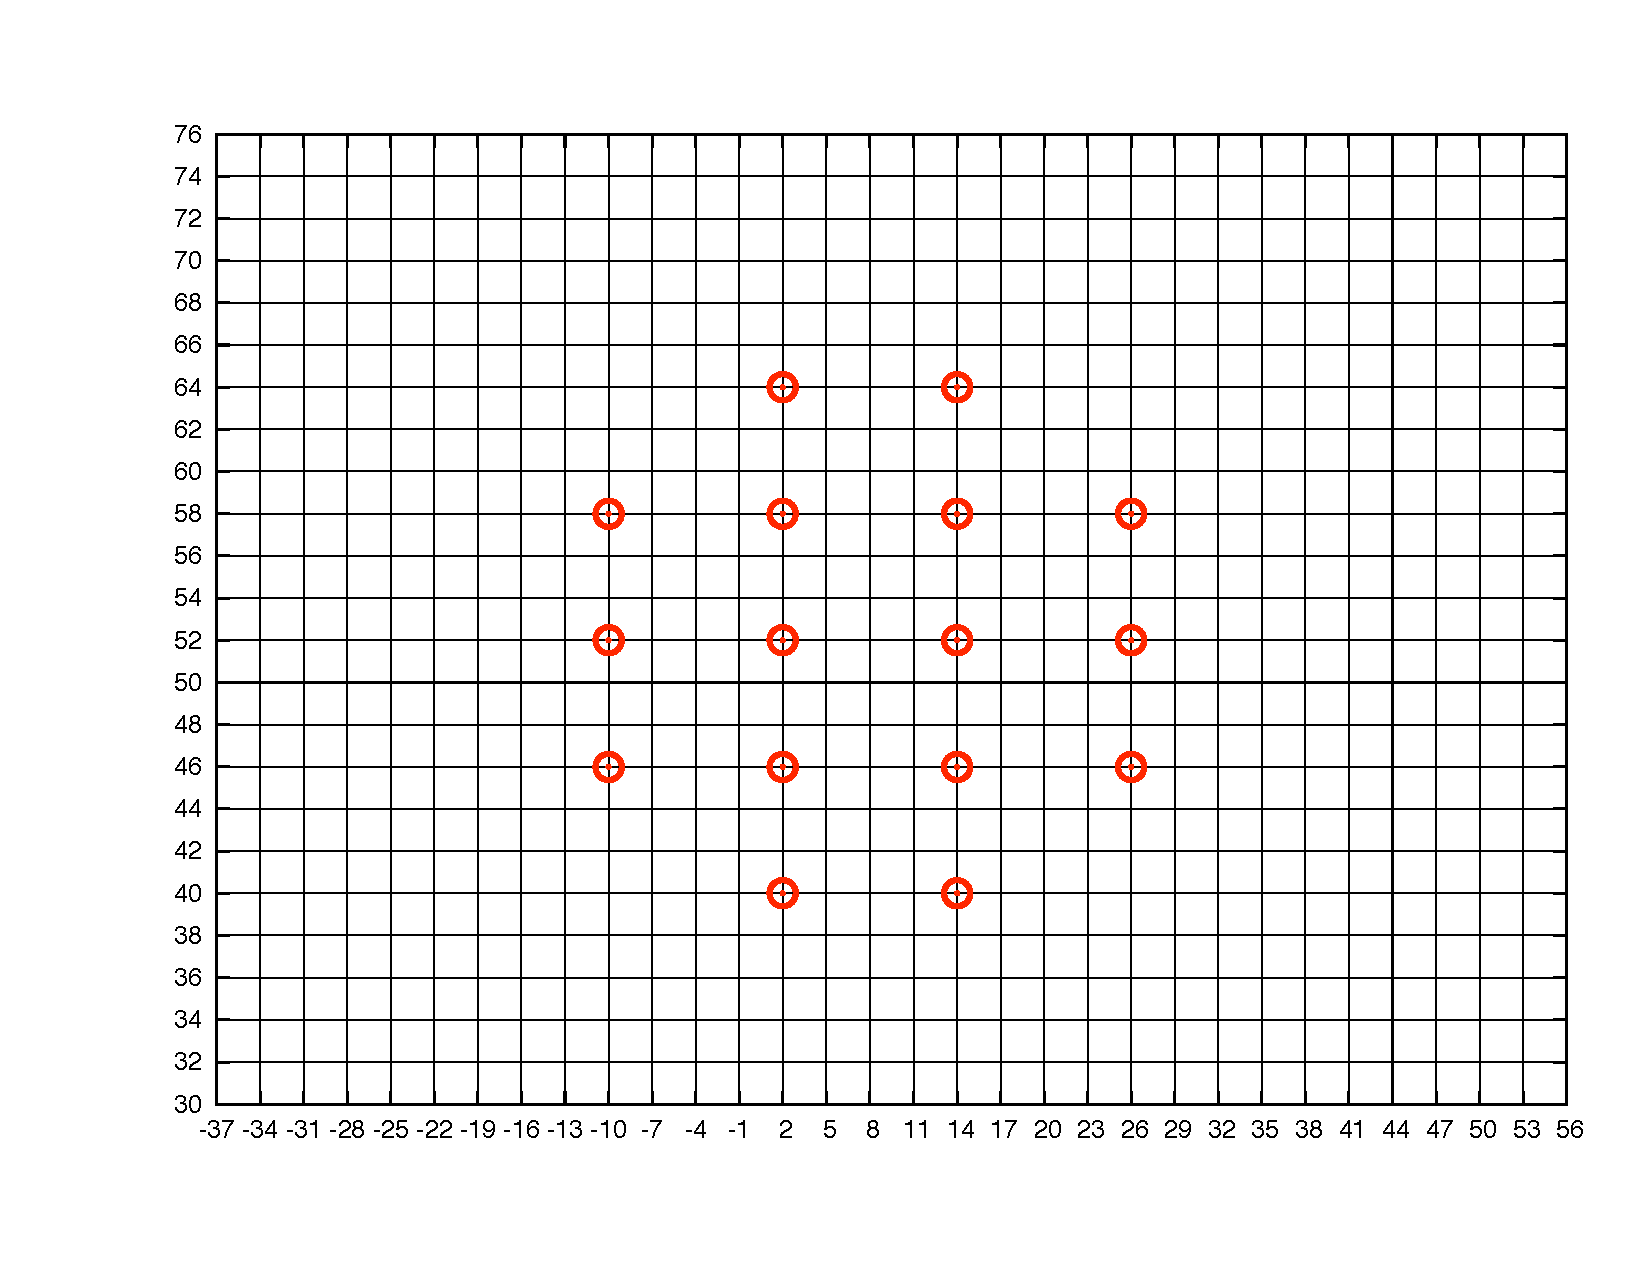
\includegraphics[width=8cm]{jct00.pdf}
\caption{
Selected grid-points (red circles) for ERA40-domain 00 [37W - 56E (32pts by 3\degree), 30N - 76N (24pts by 2\degree)]. 
37W;30N is the first position in data, 56E;76N the last. The classification grid has an extent 
of 36\degree E - W x 24\degree N - S and is centered in 8E;52N. }
\label{fig:jct00}
\end{figure}

\begin{figure}[h]
\centering
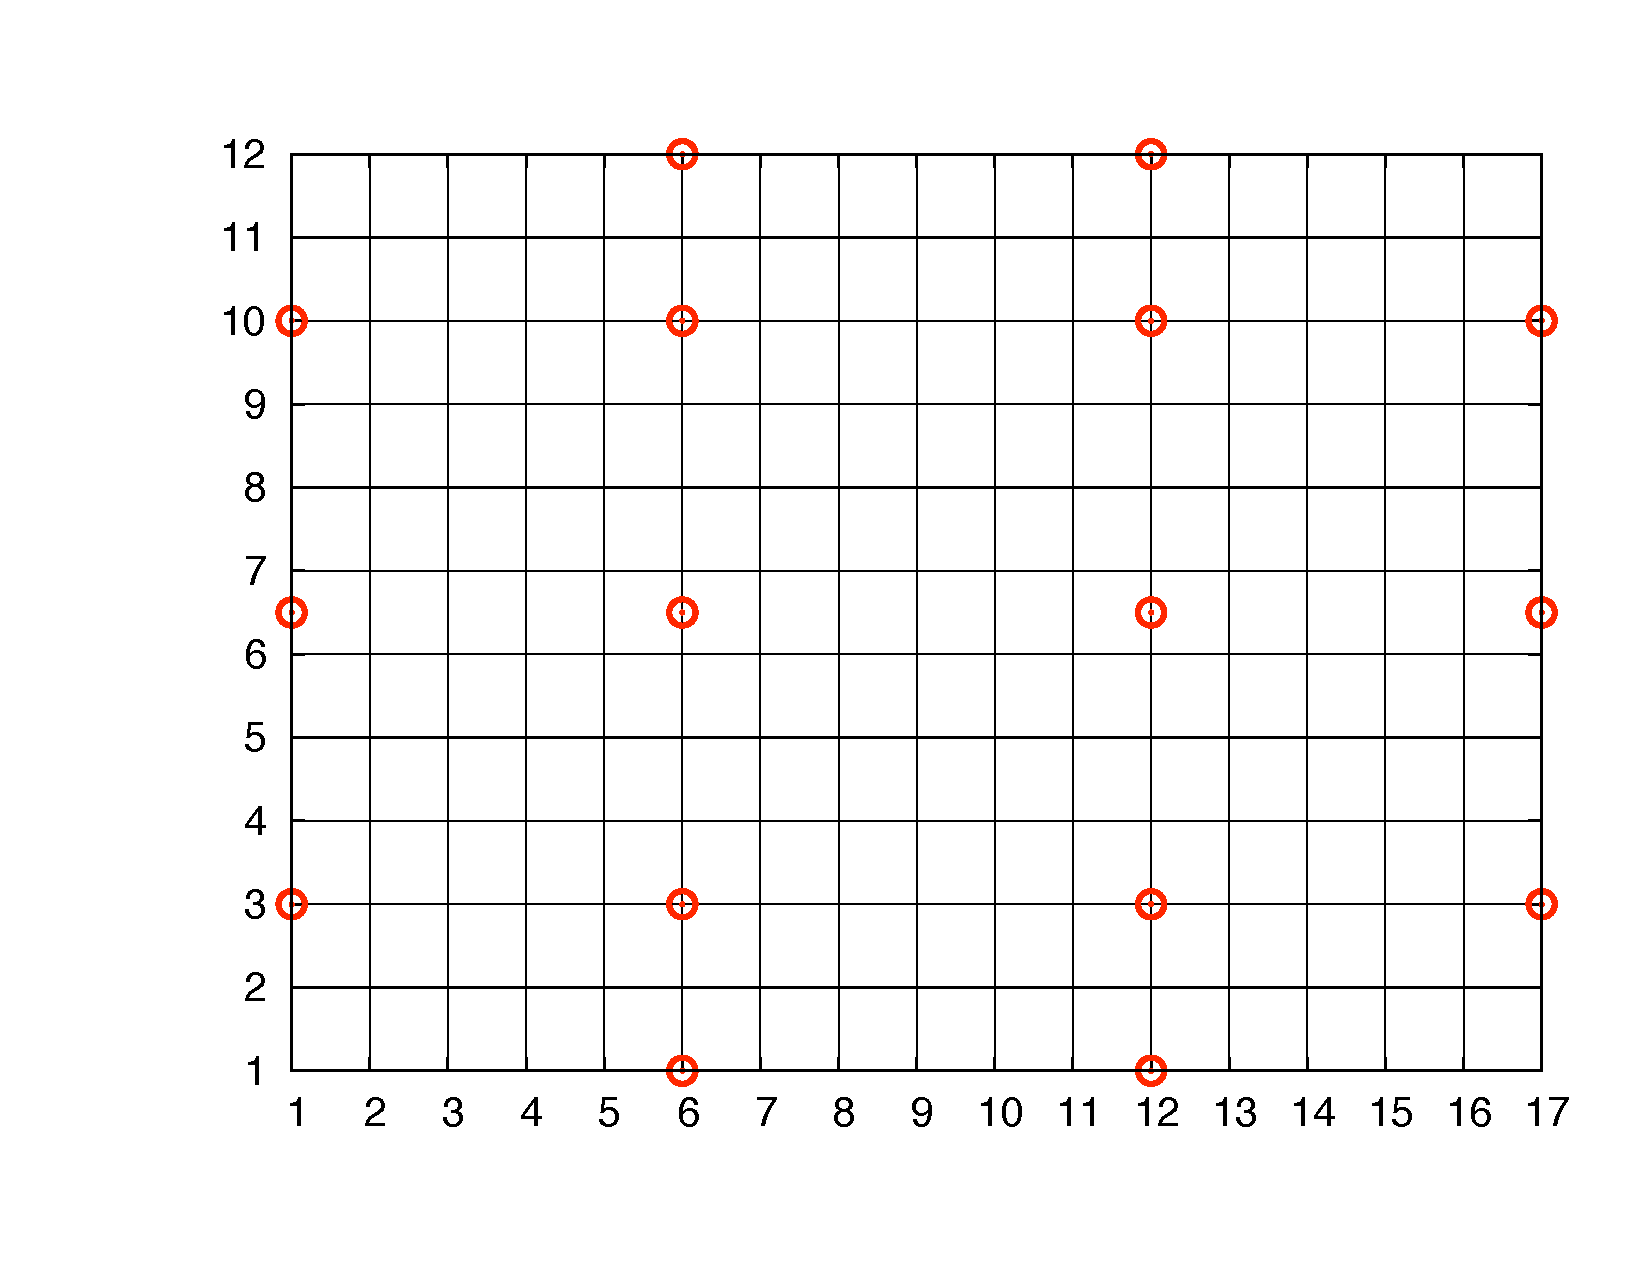
\includegraphics[width=8cm]{jct06v.pdf}
\caption{
Selected grid-points (red circles) for a 17x12 grid, if -crit 2 is used. Linear interpolation between the neighboring points is done to achieve the values for the middle line. The grid is no more equally spaced in latitudinal direction.}
\label{fig:jct06v}
\end{figure}

\begin{figure}[h]
\centering
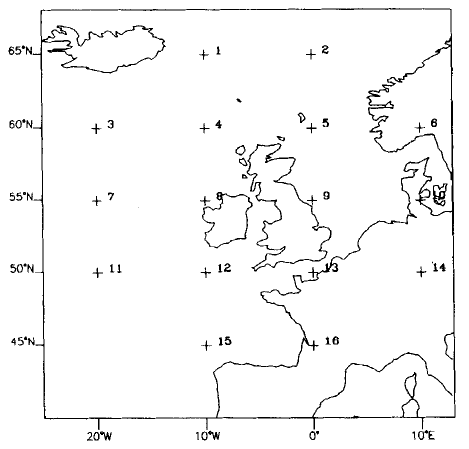
\includegraphics[width=8cm]{jones1993a.png}
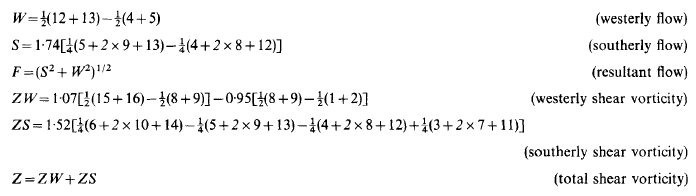
\includegraphics[width=12cm]{jones1993b.png}
\caption{
Grid point and index scheme from \citet{Jones1992}}
\label{fig:jct02}
\end{figure}

This method was developed by \citet{Jenkinson1977} and is intended to provide an objective scheme that acceptably reproduces the subjective Lamb weather types \citep{Jenkinson1977, Jones1992}. Therefore daily grid-point mean sea-level pressure data is classified as follows:
\begin{enumerate}
\item First the input data is analysed due to its grid:
  \begin{itemize}
  \item  Because the Jenkinson-Collison scheme uses 16 grid points out of a 5\degree north-south and 10\degree east-west resolved grid, with an overall extent of 20\degree x 30\degree latitude by longitude, the classification-grid has to be altered if resolution and extent of the data-grid differ (see Fig. \ref{fig:jct00}). If the data spreads a broader region, the classification-grid is centered in the middle of it. If you use -crit 2 (default is -crit 1) the classification grid is extended to the whole data region (see Fig. \ref{fig:jct06v}).
  \item Moreover the 16 grid points are chosen out of the grid; only their data is read in from the input-data-file and considered further on.
   \end{itemize}
\item In a second step the classification criteria are calculated:
  \begin{itemize}
  \item Therefore also some adjustment is done according to the relative grid-point spacings and the middle latitude of the classification region \citep{Tang2008}.
  \item Now the wind-flow characteristics are computed \citep{Jones1992}, thereafter each day's pressure pattern is represented by westerly, southerly and resultant flow, as well as westerly, southerly and total shear vorticity.
  \end{itemize}
\item Finally the classification is done. By reason of being predefined, the possible numbers of types are 8, 9, 10, 11, 12, 18, 19, 20, 26, 27 and 28, explained as follows:
  \begin{itemize}
  \item Types 1 to 8 (in 8 to 12 selected types) are using the prevailing wind directions (W, NW, N, NE, E, SE, S, and SW, where W = 1 etc.).
  \item Types 1 to 16 (in 18, 19 or 20) are a subdivision of the 8 directional types into tendentious cyclonic and anticyclonic (1-8=cyclonic, 9-16=anticyclonic).
  \item Types 1 to 24 (in 26, 27 or 28) combine mainly directions with partly cyclonic and anticyclonic ones (1-8=cyclonic, 9-16=straight, 17-24=anticyclonic).
  \item Types 9/10, 17/18 or 25/26 indicate pure cyclonic / anticyclonic days.
  \item The 9th, 11th, 19th or 27th type stands for a light indeterminate flow class and can be treated as unclassified (except for 10 types, where the 9th is something else).
  \item Type 12, 20 or 28 figures out a gale day.
  \end{itemize}
\end{enumerate}

Because the method is specialized on classifying daily mean sea-level 
pressure patterns only, some thresholds are hard coded to distinguish 
flow intensities. This is of course problematic if this method should 
be applied e.g. on geopotential heights. Therefore there are options 
modifying the default classification scheme.  

\subsubsection*{Options}
Strictly necessary options:
\begin{itemize}
 \item \verb+-dat <specification>+:\\ Input data. Grid description is necessary!
\end{itemize}
The following options define the classification:
\begin{itemize}
 \item \verb+-ncl <int>+:\\ The number of types as described above. 
 Default is 9.
\item \verb+-thres <real>+:\\ If -thres is set to 1, no "weak" flows are 
classified (class 9, 11, 19 or 27; depending on -ncl <int>). Use this for other variables than MSLP. 
\end{itemize}
Options for data output:
\begin{itemize}
 \item \verb+-cla <filename>+:\\ Output file name for the classification catalog.
 \item \verb+-dcol <int>+:\\ Number of date columns in the classification catalog.
 \item \verb+-cnt <filename>+:\\ Output file name for the class centroids.
 \item \verb+-idx <basename>+:\\ Output base name for values of wind-flow 
 characteristics (w/s/f=westerly/southerly/resultant flow, zw/zs/z=westerly/southerly/total shear vorticity).
\end{itemize}

\subsubsection*{Output}
This method returns one file containing the classification catalog. 
Overall class centroids as well as a file containing values of wind-flow 
characteristics are optional.

\subsubsection*{Examples}
An example with default values:
\begin{lstlisting}
cost733class /*-dat/* /+pth:/+slp.dat /+fmt:/+ascii /+lon:/+-10:30:2.5 /+lat:/+35:60:2.5 /+fdt:/+2000:1:1:12 /+ldt:/+2008:12:31:12 /+ddt:/+1d /--met/- JCT /--ncl/- 9 /*-cla/* JCT09.cla /*-dcol/* 3 
\end{lstlisting}
Another example:
\begin{lstlisting}
cost733class /*-dat/* /+pth:/+slp.dat /+fmt:/+ascii /+lon:/+-10:30:2.5 /+lat:/+35:60:2.5 /+fdt:/+2000:1:1:12 /+ldt:/+2008:12:31:12 /+ddt:/+1d /--met/- JCT /--ncl/- 26 /--idx/- JCT26  /*-cla/* JCT26.cla /*-dcol/* 3 
\end{lstlisting}
Same but with a different number of classes and output for values of wind-flow characteristics.
%Because the method is specialized on classifying daily mean sea-level pressure patterns only, some thresholds are hardcoded to distinguish flow intensities. This is of course problematic if this method should be applied e.g. on geopotential heights. Therefore there are the following options modifying the default classification scheme:
%\begin{itemize}
%\item \verb+-thres <real>+: \\
	%If -thres is set to 1, no "weak" flows are classified (class 9, 11, 19 or 27; depending on -ncl <int>). Use this for other variables than MSLP.
%\end{itemize}

%%%%%%%%%%%%%%%%%%%%%%%%%%%%%%%%%%%%%%%%%%%%%%%%%%%%%%%%%%%%%%%%%%%%%%%%
\subsection{WLK | wlk - automatic weather type classification according to German metservice}


This method is based on the OWLK (objective weather type classification) by \citet{Dittmann1995} and \citet{Bissolli2003}, originally including 40 different types. The types are defined according to the wind field (U and V) of a certain level, as well as according to cyclonicity of pressure fields of a first and a second level and according to total precipitable water, the latter (cyclonicity and water) only if the corresponding data sets are provided at the command line. 
In comparison to the initial OWLK method the recent classification WLKC733 which is included in cost733cat provides a few simplifications regarding output parameters \citep[see][]{Philipp2010}.

The alphanumeric output consists of five letters: the first two letters denote the flow pattern in terms of a dominant wind sector counting clockwise, i.e. 01 = NE, 02 = SE, 03 = SW, 04 = NW and 00 = undefined (varying directions). For determination of the dominant wind sector the true wind direction obtained from U and V-components at 700 hPa is used and circulation patterns are derived from a simple majority (threshold) of the weighted wind field vectors at 700 hPa. If no majority could be found, the class 00 will be selected. For counting the respective wind directions a weighting mask, putting higher weights on grid points in the center of the domain, is applied.

The third and fourth letter denote Anticyclonicity or Cyclonicity at 925 hPa and 500 hPa, respectively, based on the weighted mean value of the quasi-geostrophic vorticity, again putting higher weights on central grid points. 
The fifth letter denotes Dry or Wet conditions, according to an weighted area mean value of the towering water content (whole atmospheric column) which is compared to the long-term daily mean. 

In order to achieve a classification system for 28 types (WLKC28) six main wind sector types are used (01 = 330-30\degree and so on in 60\degree steps) plus one undefined type, which are further discriminated by cyclonicity as described above. 
18 types (WLKC18) are produced by using nine wind sector types (sector 01 = 345-15\degree, 02 = 15-75\degree, 03 = 75-105\degree, 04 = 105-165\degree, 05 = 165-195\degree, 06 = 195-255\degree, 07 = 255-285\degree, 08 = 285-345\degree, 00 = undefined) and cyclonicity at 925 hPa, while the latter is omitted for producing nine types (WLKC09).

The third and fourth letter denoting cyclonicity of pressure fields of a first and a second level, and total precipitable water, respectively, are analyzed only if the corresponding data sets are provided at the command line. Thus the order of the data sets provided by the command line arguments plays an important role for this method. 

It is important to note that any other meteorological parameters than U and V for the first two data fields do 
not make any sense for this method!

For determination of the main wind sector and cyclonicity a weigthing mask is applied to the input fields putting
highest weights on the central zone, intermediate weight to the middle zone and lowest weight to the margin zone.
The mask is shown on verbose level > 1.

Since within this method the number of types is defined by the number of wind sectors and the input data the 
\verb+-ncl+ flag can be omitted and is ignored.

\subsubsection*{Options}
Strictly necessary options:
\begin{enumerate}
 \item \verb+-dat <specification>+:\\ Input data for U-component at the 700 hPa level. Grid description is 
 necessary!
 \item \verb+-dat <specification>+:\\ Input data for V-component at the 700 hPa level. Grid description is 
 necessary!
\end{enumerate}
Optional data input:
\begin{enumerate}
 \setcounter{enumi}{2}
 \item \verb+-dat <specification>+:\\ Input data for geopotential at the 925 hPa level. Grid description is 
 necessary!
 \item \verb+-dat <specification>+:\\ Input data for geopotential at the 500 hPa level. Grid description is 
 necessary!
 \item \verb+-dat <specification>+:\\ Input data for towering water content (whole atmospheric column). Grid description is 
 necessary!
\end{enumerate}
There are several special flags controlling the wlk classification (beside the control via input data sets):
\begin{itemize}
\item \verb+-step <integer>+: \\
	The number of wind sectors. The 360$\circ$ of the wind rose will be divided by \verb+<integer>+ to 
	determine the threshold angle for the different wind sectors.
\item \verb+-shift+: \\
	Shift the sectors defined by \verb+-step <integer>+ by half of the angle. I.e. North will be in the
	center of sector.
\item \verb+-thres <real>+: \\
	fraction of grid points for decision on main wind sector (default=0.6)
\item \verb+-alpha <real>+: \\
	central weight for weighting mask (default=3.D0)
\item \verb+-beta <real>+: \\
	middle zone weight for weighting mask (default=2.D0)
\item \verb+-gamma <real>+: \\
	margin zone weight for weighting mask (default=1.D0)
\item \verb+-delta <real>+: \\
	width factor for weighting zones (nx*delta|ny*delta) (default=0.2)
\end{itemize}
Options for data output:
\begin{itemize}
 \item \verb+-cla <filename>+:\\ Output file name for the classification catalog.
 \item \verb+-dcol <int>+:\\ Number of date columns in the classification catalog.
 \item \verb+-cnt <filename>+:\\ Output file name for the class centroids.
 \item \verb+-idx <filename>+:\\ Output file name for values of main wind sector, cyclonicity (925 and 500 hPa level) and total precipitable water.
\end{itemize}

\subsubsection*{Output}
This method returns one file containing the classification catalog. 
Overall, per parameter class centroids as well as a file containing values of wind-flow 
characteristics and precipitable water are optional.

\subsubsection*{Examples}
For example a classification with the maximum number of data set fields and a division into 8 wind sectors:
\begin{scriptsize}
\begin{lstlisting}
cost733class \
/*-dat/* /+pth:/+era40_U700_12Z_195709-200208.domain00.dat /+lon:/+-37:56:3 /+lat:/+30:76:2 \
/*-dat/* /+pth:/+era40_V700_12Z_195709-200208.domain00.dat /+lon:/+-37:56:3 /+lat:/+30:76:2 \
/*-dat/* /+pth:/+era40_Z925_12Z_195709-200208.domain00.dat /+lon:/+-37:56:3 /+lat:/+30:76:2 \
/*-dat/* /+pth:/+era40_Z500_12Z_195709-200208.domain00.dat /+lon:/+-37:56:3 /+lat:/+30:76:2 \
/*-dat/* /+pth:/+era40_TWC_12Z_195709-200208.domain00.dat /+lon:/+-37:56:3 /+lat:/+30:76:2 \
/--met/- wlk /--step/- 8 
\end{lstlisting}
\end{scriptsize}

Another more advanced example omitting the moisture index could be:
\begin{scriptsize}
\begin{lstlisting}
cost733class \
/*-dat/* /+pth:/+/alcc/ptmp/geodata/ERA40/ascii/era40_U700_12Z_195709-200208.domain00.dat \
	/+lon:/+-37:56:3 /+lat:/+30:76:2 \
/*-dat/* /+pth:/+/alcc/ptmp/geodata/ERA40/ascii/era40_V700_12Z_195709-200208.domain00.dat \
	/+lon:/+-37:56:3 /+lat:/+30:76:2 \
/*-dat/* /+pth:/+/alcc/ptmp/geodata/ERA40/ascii/era40_Z925_12Z_195709-200208.domain00.dat \
	/+lon:/+-37:56:3 /+lat:/+30:76:2 \
/*-dat/* /+pth:/+/alcc/ptmp/geodata/ERA40/ascii/era40_Z500_12Z_195709-200208.domain00.dat \
	/+lon:/+-37:56:3 /+lat:/+30:76:2 \
/--met/- WLK /--step/- 8 /--shift/- /--thres/- 0.35 /--crit/- 0 /--alpha/- 7 /--delta/- 0.15 \
/--idx/- WLK09_YR_S01_U7-V7_D00.txt
\end{lstlisting}
\end{scriptsize}

producing the output:
\begin{scriptsize}
\begin{lstlisting}
starting cost733class ...
 method  = WLK
 ncl     =  27
 period  = era40
 months  = 1,2,3,4,5,6,7,8,9,10,11,12
 hours   = 00,06,12,18
 verbose =   2

 data input ...
 applyweighting = T
 writedat       = F
 writestd       = F
 npar     =  4
 got    16436 lines from era40_U700_12Z_195709-200208.domain00.dat, done!
 got    16436 lines from era40_V700_12Z_195709-200208.domain00.dat, done!
 got    16436 lines from era40_Z925_12Z_195709-200208.domain00.dat, done!
 got    16436 lines from era40_Z500_12Z_195709-200208.domain00.dat, done!

 calling wlk ...
 number of windir sectors         =           6
 fraction of gridpoint wind       =  0.350000000000000     
 anomalies of cyclonicity (1=yes) =           0
 shift sectors centering to 0 deg = T
 central weight alpha             =   7.00000000000000     
 middle weight beta               =   2.00000000000000     
 margin weight gamma              =   1.00000000000000     
 mask zone width factor delta     =  0.150000000000000     
 grids for U and V have size    32 by    24
 
 weight mask:
1.1.1.1.1.1.1.1.1.1.1.1.1.1.1.1.1.1.1.1.1.1.1.1.1.1.1.1.1.1.1.1.
1.1.1.1.1.1.1.1.1.1.1.1.1.1.1.1.1.1.1.1.1.1.1.1.1.1.1.1.1.1.1.1.
1.1.1.1.1.1.1.1.1.1.1.1.1.1.1.1.1.1.1.1.1.1.1.1.1.1.1.1.1.1.1.1.
1.1.1.1.2.2.2.2.2.2.2.2.2.2.2.2.2.2.2.2.2.2.2.2.2.2.2.2.1.1.1.1.
1.1.1.1.2.2.2.2.2.2.2.2.2.2.2.2.2.2.2.2.2.2.2.2.2.2.2.2.1.1.1.1.
1.1.1.1.2.2.2.2.2.2.2.2.2.2.2.2.2.2.2.2.2.2.2.2.2.2.2.2.1.1.1.1.
1.1.1.1.2.2.2.2.2.2.2.2.2.2.2.2.2.2.2.2.2.2.2.2.2.2.2.2.1.1.1.1.
1.1.1.1.2.2.2.2.2.7.7.7.7.7.7.7.7.7.7.7.7.7.7.2.2.2.2.2.1.1.1.1.
1.1.1.1.2.2.2.2.2.7.7.7.7.7.7.7.7.7.7.7.7.7.7.2.2.2.2.2.1.1.1.1.
1.1.1.1.2.2.2.2.2.7.7.7.7.7.7.7.7.7.7.7.7.7.7.2.2.2.2.2.1.1.1.1.
1.1.1.1.2.2.2.2.2.7.7.7.7.7.7.7.7.7.7.7.7.7.7.2.2.2.2.2.1.1.1.1.
1.1.1.1.2.2.2.2.2.7.7.7.7.7.7.7.7.7.7.7.7.7.7.2.2.2.2.2.1.1.1.1.
1.1.1.1.2.2.2.2.2.7.7.7.7.7.7.7.7.7.7.7.7.7.7.2.2.2.2.2.1.1.1.1.
1.1.1.1.2.2.2.2.2.7.7.7.7.7.7.7.7.7.7.7.7.7.7.2.2.2.2.2.1.1.1.1.
1.1.1.1.2.2.2.2.2.7.7.7.7.7.7.7.7.7.7.7.7.7.7.2.2.2.2.2.1.1.1.1.
1.1.1.1.2.2.2.2.2.7.7.7.7.7.7.7.7.7.7.7.7.7.7.2.2.2.2.2.1.1.1.1.
1.1.1.1.2.2.2.2.2.7.7.7.7.7.7.7.7.7.7.7.7.7.7.2.2.2.2.2.1.1.1.1.
1.1.1.1.2.2.2.2.2.2.2.2.2.2.2.2.2.2.2.2.2.2.2.2.2.2.2.2.1.1.1.1.
1.1.1.1.2.2.2.2.2.2.2.2.2.2.2.2.2.2.2.2.2.2.2.2.2.2.2.2.1.1.1.1.
1.1.1.1.2.2.2.2.2.2.2.2.2.2.2.2.2.2.2.2.2.2.2.2.2.2.2.2.1.1.1.1.
1.1.1.1.2.2.2.2.2.2.2.2.2.2.2.2.2.2.2.2.2.2.2.2.2.2.2.2.1.1.1.1.
1.1.1.1.1.1.1.1.1.1.1.1.1.1.1.1.1.1.1.1.1.1.1.1.1.1.1.1.1.1.1.1.
1.1.1.1.1.1.1.1.1.1.1.1.1.1.1.1.1.1.1.1.1.1.1.1.1.1.1.1.1.1.1.1.
1.1.1.1.1.1.1.1.1.1.1.1.1.1.1.1.1.1.1.1.1.1.1.1.1.1.1.1.1.1.1.1.
 divided z925 by 10, min, max =   4.57263000000000        1062.87168000000     
 divided z500 by 10, min, max =   4471.24336000000        5913.77969000000     
 number of classes =          28
 
     1   00AAx -9999.9 -9999.9         402
     2   01AAx   330.0    30.0         294
     3   02AAx    30.0    90.0          80
     4   03AAx    90.0   150.0         117
     5   04AAx   150.0   210.0         443
     6   05AAx   210.0   270.0        3690
     7   06AAx   270.0   330.0        2308
     8   00ACx -9999.9 -9999.9          35
     9   01ACx   330.0    30.0          85
    10   02ACx    30.0    90.0          19
    11   03ACx    90.0   150.0           7
    12   04ACx   150.0   210.0          60
    13   05ACx   210.0   270.0         802
    14   06ACx   270.0   330.0         695
    15   00CAx -9999.9 -9999.9          15
    16   01CAx   330.0    30.0          11
    17   02CAx    30.0    90.0           1
    18   03CAx    90.0   150.0           5
    19   04CAx   150.0   210.0          78
    20   05CAx   210.0   270.0        1187
    21   06CAx   270.0   330.0         584
    22   00CCx -9999.9 -9999.9          40
    23   01CCx   330.0    30.0          69
    24   02CCx    30.0    90.0           2
    25   03CCx    90.0   150.0           5
    26   04CCx   150.0   210.0         145
    27   05CCx   210.0   270.0        3205
    28   06CCx   270.0   330.0        2052
 
 catalog output = WLK27_YR_S01_U7-V7-Z9-Z5_D00.txt       16436

 final result:
         WLK ecv = 0.138173112002  csize =   402   294    80   117   443  3690  2308    
         35    85    19     7    60   802   695    15    11     1     5    78  1187  
         584    40    69     2     5   145  3205  2052
\end{lstlisting}
\end{scriptsize}

%%%%%%%%%%%%%%%%%%%%%%%%%%%%%%%%%%%%%%%%%%%%%%%%%%%%%%%%%%%%%%%%%%%%%%%%
\section{Methods based on Eigenvectors}

cost733class contains source code to calculate the eigenvectors of the input data set by singular value 
decomposition.

%%%%%%%%%%%%%%%%%%%%%%%%%%%%%%%%%%%%%%%%%%%%%%%%%%%%%%%%%%%%%%%%%%%%%%%%
\subsection{PCT | tpca - t-mode principal component analysis using oblique rotation}

The classification by obliquely rotated Principal Components in T-mode (PCT) (also called TPCA, Principal Component Analysis in T-mode) is based on \citet{Huth2000}. With regard to computer resources, and simultaneously to speed up the calculation of the PCA, the data is split into subsets. Consequently, the principal components obtained for each subset are projected onto the rest of data.
\begin{enumerate}
\item The Data is standardized spatially: each pattern's mean is subtracted from the data; then the patterns are divided by their standard deviations.
\item The data is split into ten subsets: selecting the 1st, 11th, 21st, 31st, 41st, etc. pattern as the first subset; the 2nd, 12th, 22nd, 32nd, 42nd, etc. as the second subset, and so on.
\item In order to achieve the principal components the algorithm based on the singular value decomposition is used.
\item The definition of the numbers of principal components in cost733class is in contrast to the original scheme, where the scree-plot method is used, defined by the user (-ncl).
\item An oblique rotation (using direct oblimin) is applied on the principal components, employing a FORTRAN90 adaptation of the GPA (Gradient Projection Algorithm) according to \citet{Bernaards2005}.
\item The principal components are mirrored, thereafter the respective maximum absolute loadings are positive.
\item The projection of the principal component scores of each subset onto the remaining data is realized by calculating the Pearson correlation coefficients between the data and the scores.
\item To evaluate the ten classifications based on the subsets, contingency tables are used. Subsequently CHI-square is calculated between each subset's types (every subset solution is compared with the other nine ones). The subset which gains the highest sum (of the nine comparisons) is selected, and only its types are returned.
\end{enumerate}

\subsubsection*{Options}
Strictly necessary options:
\begin{itemize}
 \item \verb+-dat <specification>+:\\ Input data. No grid description is necessary.
\end{itemize}
The following options define the classification:
\begin{itemize}
 \item \verb+-ncl <int>+:\\ Determine the number of principal components. Default is 9.
\end{itemize}
Options for data output:
\begin{itemize}
 \item \verb+-cla <filename>+:\\ Output file name for the classification catalog.
 \item \verb+-dcol <int>+:\\ Number of date columns in the classification catalog.
 \item \verb+-cnt <filename>+:\\ Output file name for the class centroids.
 \item \verb+-idx <basename>+:\\ Output base name for scores (*.sco), loadings (*.ldg), explained variances (*.exv) and total variance(*.tvr) of the rotated principal components (step 6), correlation values (*.cor) of original data and subset scores (step 7) and subset classifications (*sub.cla).
\end{itemize}

\subsubsection*{Output}
This method returns one file containing the classification catalog. 
Overall class centroids as well as files containing results from various intermediate steps are optional.

\subsubsection*{Examples}
An example with default values:
\begin{lstlisting}
cost733class /*-dat/* /+pth:/+slp.dat /+fmt:/+ascii /+lon:/+-10:30:2.5 /+lat:/+35:60:2.5 /+fdt:/+2000:1:1:12 /+ldt:/+2008:12:31:12 /+ddt:/+1d /--met/- PCT /--ncl/- 9 /*-cla/* PCT09.cla /*-dcol/* 3 
\end{lstlisting}
Another example with additional output files and a different number of principal components:
\begin{lstlisting}
cost733class /*-dat/* /+pth:/+slp.dat /+fmt:/+ascii /+lon:/+-10:30:2.5 /+lat:/+35:60:2.5 /+fdt:/+2000:1:1:12 /+ldt:/+2008:12:31:12 /+ddt:/+1d /--met/- PCT /--ncl/- 4 /--idx/- PCT04 /*-cla/* PCT04.cla /*-dcol/* 3 
\end{lstlisting}

%%%%%%%%%%%%%%%%%%%%%%%%%%%%%%%%%%%%%%%%%%%%%%%%%%%%%%%%%%%%%%%%%%%%%%%%
\subsection{PTT | tpcat - t-mode principal component analysis using orthogonal rotation}
\verb+PTT+ is a simplified variant of t-mode principal component analysis with subsequent assignment of the cases to the PC with the maximum loading. Since there is no split into sub samples the amount of computer memory is relatively high as well as the run time. In contrast to \verb+PCT+ the PCs are rotated orthogonally. 

\subsubsection*{Options}
Strictly necessary options:
\begin{itemize}
 \item \verb+-dat <specification>+:\\ Input data. No grid description is necessary.
\end{itemize}
The following options define the classification:
\begin{itemize}
 \item \verb+-ncl <int>+:\\ Determine the number of principal components. Default is 9.
\end{itemize}
Options for data output:
\begin{itemize}
 \item \verb+-cla <filename>+:\\ Output file name for the classification catalog.
 \item \verb+-dcol <int>+:\\ Number of date columns in the classification catalog.
 \item \verb+-cnt <filename>+:\\ Output file name for the class centroids.
 \item \verb+-idx <basename>+:\\ Output base name for scores (*.sco) and loadings (*.ldg).
\end{itemize}

\subsubsection*{Output}
This method returns one file containing the classification catalog. 
Overall class centroids as well as files containing results from intermediate steps are optional.

\subsubsection*{Examples}
An example with default values:
\begin{lstlisting}
cost733class /*-dat/* /+pth:/+slp.dat /+fmt:/+ascii /+lon:/+-10:30:2.5 /+lat:/+35:60:2.5 /+fdt:/+2000:1:1:12 /+ldt:/+2008:12:31:12 /+ddt:/+1d /--met/- PTT /--ncl/- 9 /*-cla/* PTT09.cla /*-dcol/* 3 
\end{lstlisting}
Another example with additional output files and a different number of principal components:
\begin{lstlisting}
cost733class /*-dat/* /+pth:/+slp.dat /+fmt:/+ascii /+lon:/+-10:30:2.5 /+lat:/+35:60:2.5 /+fdt:/+2000:1:1:12 /+ldt:/+2008:12:31:12 /+ddt:/+1d /--met/- PTT /--ncl/- 4 /--idx/- PTT04 /*-cla/* PTT04.cla /*-dcol/* 3 
\end{lstlisting}

%%%%%%%%%%%%%%%%%%%%%%%%%%%%%%%%%%%%%%%%%%%%%%%%%%%%%%%%%%%%%%%%%%%%%%%%
\subsection{PXE | pcaxtr - the extreme score method}

%This method defines key group patterns by extremely high and low scores of a s-mode Principal Component Analysis.
%For each PC the cases of extremely high scores (scores above threshold +/-2.0 by default) are determined. No other PC
%is allowed to exceed a score limit (of +/-1.0 by default) in order to find cases dominated by the PC in question.

This methodological approach has as main goal to use Principal Component Analysis as an objective way for obtaining the number of circulation types (CT hereafter) and its initial centroids that our final classification will have. 

The general procedure does not vary with respect to the usual outline of PCA: S-mode structure (grid points as the columns and cases as the rows of the matrix), use of the correlation matrix to obtain the new variables, and orthogonal rotation (Varimax) to better adjust the result to the climatic reality. There are few novelties: 

\begin{itemize}
\item spatial standardization of the gridded data before the PCA procedure.
\item after aplying PCA, the use of a rule (the extreme scores) which by being fulfilled or not by each original case, leads to the final number of CTs and their centroids.
\end{itemize}

Thus, based on those cases of our sample that according to their scores show a spatial structure similar to some rotated PC (cases with high score values with respect to that component, i.e higher/lower than +2/-2 respectively, and lower scores for the rest of the PCs, i.e. between +2 and -2) we obtain the centroids for each component and phase (positive/negative). These are then our provisional CTs, with clear climatic meaning since they derive from the real data (existence in the reality of the spatial patterns identified by the PCA). Despite that, in case that a PC does not have any real case (that fulfills the rule of the extremes scores) assigned to it, this spatial pattern is considered as a statistical artifact; this theoretical CT according to PCA is eliminated and the final number of CTs of the classification diminishes. 

Finally, to assign each case of the sample to one of the CTs, the euclidean distance is used. This is calculated using the multivariate coordinates of each case expressed by its scores, and the location in the PC space of the centroid of each CT. Obviously, these centroids (and number of clusters) can also be used as initial seeds for an optimization algorithm like K-means (see method PCAXTRKM - PXK). Once the entire sample has been classified, we have our catalog of final CTs. For more details about the rule of the "extreme scores" see Esteban el al 2006 and Philipp el al 2010. 

We could say that this approach is an attempt to reproduce the T-mode PCA approach, that uses the coefficients obtained with PCA (correlations) for distributing the cases among the different groups considered. PXE employs the PC-scores to do this assignment, reducing substantially the calculation requirements. On the contrary, some uncertainty is introduced by the use of a similarity threshold based on the PC-scores (normally -2 /+ 2), thus the suitability of this threshold value depends on the variability of the sample. The normally used  -2 /+ 2 can be inappropriate for samples with very few cases or with little variability, being recommendable to change to, for example, a -1 /+ 1 threshold (see Esteban et al 2005). 

\subsubsection*{Options}
Strictly necessary options:
\begin{itemize}
 \item \verb+-dat <specification>+:\\ Input data. No grid description is necessary.
\end{itemize}
The following options define the classification:
\begin{itemize}
 \item \verb+-ncl <int>+:\\ Determine the number of classes. Has to be always an even number (2, 4, 8, 10,...). Note, however, that sometimes not all classes are realized, possibly leading to empty (less) types. Default is 10.
 \item \verb+-niter <int>+ : Maximum number of iterations. Use \verb+-niter 0+ (the default) for direct assignment of cases using the Euclidean distance. Use \verb+-niter >0+ for a k-means cluster analysis like \verb+-met KMN+ but with starting partitions derived by \verb+PXE+.
 \item \verb+-crit <int>+: \\Further relevant switch concerning the normalization method of the input data before the PCA is performed. \verb+<int>+ can be:
 \begin{itemize}
  \item[0]: Only normalize patterns for PCA (original)
  \item[1]: Normalize patterns and normalize grid point values afterwards (default)
  \item[2]: Normalize patterns and center grid point values afterwards
 \end{itemize}
 \item \verb+-thres <real>+: \\
	Definition of extreme score cases. Threshold defining key group (default=2.0)
 \item \verb+-delta <real>+: \\
	Definition of extreme score cases. Score limit for other PCs to define uniquely leading PC (default 1.0)
\end{itemize}
Options for data output:
\begin{itemize}
 \item \verb+-cla <filename>+:\\ Output file name for the classification catalog.
 \item \verb+-dcol <int>+:\\ Number of date columns in the classification catalog.
 \item \verb+-cnt <filename>+:\\ Output file name for the class centroids.
 \item \verb+-idx <basename>+:\\ Output base name for rotated scores (*.sco).
\end{itemize}

\subsubsection*{Output}
This method returns one file containing the classification catalog. 
Overall class centroids as well as files containing results from intermediate steps are optional.

\subsubsection*{Examples}
An example with default values:
\begin{lstlisting}
cost733class /*-dat/* /+pth:/+slp.dat /+fmt:/+ascii /+lon:/+-10:30:2.5 /+lat:/+35:60:2.5 /+fdt:/+2000:1:1:12 /+ldt:/+2008:12:31:12 /+ddt:/+1d /--met/- PXE /--ncl/- 10 /--niter/- 0 /--thres/- 2.0 /--delta/- 1.0 /*-cla/* PXE10.cla /*-dcol/* 3 
\end{lstlisting}
Another example with additional output files and a different number of principal components:
\begin{lstlisting}
cost733class /*-dat/* /+pth:/+slp.dat /+fmt:/+ascii /+lon:/+-10:30:2.5 /+lat:/+35:60:2.5 /+fdt:/+2000:1:1:12 /+ldt:/+2008:12:31:12 /+ddt:/+1d /--met/- PXE /--ncl/- 4 /--niter/- 0 /--thres/- 2.0 /--delta/- 1.0 /--idx/- PXE /*-cla/* PXE04.cla /*-dcol/* 3 
\end{lstlisting}

%%%%%%%%%%%%%%%%%%%%%%%%%%%%%%%%%%%%%%%%%%%%%%%%%%%%%%%%%%%%%%%%%%%%%%%%
\subsection{KRZ | kruiz - Kruizingas PCA-based types}

P27 is a simple eigenvector based classification scheme \citep{Kruizinga1979,Buishand1997}. The scheme uses daily 500 hPa GPH on a regular grid (original one 6 x 6 points with the step of 5\degree in latitude and 10\degree in longitude). The actual 500 hPa height, htq, for the day t at grid point q is reduced first by subtracting the daily average height, ht, over the grid. This operation removes a substantial part of the annual cycle. The reduced 500 hPa heights ptq, are given by: 
ptq= htq - ht , q = 1,... n; n is the number of grid points, t = 1,...N, N the number of days. 

The vector of reduced 500 hPa heights is approximated as: 

pt = s1t*a1+ s2t*a2 + s3t*a3, t = 1,...N. 

a-s are the first three principal component vectors (eigenvectors of the second-moment matrix of pt) and s-s are their amplitudes or scores. 

The flow pattern of a particular day is described by three amplitudes: s1t, s2t, s3t 

	s1t*a1 characterizes the east-west component of the flow 

	s2t*a2 the north-south component and 

	s3t*a3 the cyclonicity (or anticyclonicity) 

In the original classification, the range of every amplitude is divided into three equiprobable intervals and that gives 27 classes as each pressure pattern is on the basis of its amplitudes uniquely assigned to one of the 3 x 3 x 3 possible interval combinations.

\subsubsection*{Options}
Strictly necessary options:
\begin{itemize}
 \item \verb+-dat <specification>+:\\ Input data. No grid description is necessary.
\end{itemize}
The following options define the classification:
\begin{itemize}
 \item \verb+-ncl <int>+:\\ Determine the number of classes. Valid values for \verb+<int>+ are 8,9,12,18,27,30.
\end{itemize}
Options for data output:
\begin{itemize}
 \item \verb+-cla <filename>+:\\ Output file name for the classification catalog.
 \item \verb+-dcol <int>+:\\ Number of date columns in the classification catalog.
 \item \verb+-cnt <filename>+:\\ Output file name for the class centroids.
\end{itemize}

\subsubsection*{Output}
This method returns one file containing the classification catalog. 
Overall class centroids are optional.

\subsubsection*{Examples}
An example command could be:
\begin{lstlisting}
cost733class /*-dat/* /+pth:/+hgt500.dat /--met/- KRZ /--ncl/- 27 /*-v/* 2
\end{lstlisting}

For producing 8 types the three amplitudes are divided into two intervals, which is indicated by the 
standard output on verbosity level 2.

\begin{scriptsize}
\begin{lstlisting}
 : pc = number of principal component
 : n = equiprobable intervalls per pc
 : i = number of percentile
 : s = percentile (in percent)
 : p = percentile as in timeseries
 : c = shifts class

 pc  n  i         s         p  c
  1  2  1  50.00000  -0.86810  4
  2  2  1  50.00000  -0.03095  2
  3  2  1  50.00000   0.07110  1
\end{lstlisting}
\end{scriptsize}

Thus observations of type 1 to 4 have scores below or equal to -0.86810 (the median) for PC 1 and those of type 5 to 8
have scores above -0.86810 in this example. Types 3,4 and 7,8 also have scores above -0.03095 for the second PC 
while types 1,2 and 5,6 have lower amplitudes. Types 1,3,5,7 have lower amplitudes for PC 3 than 0.07110, and
types 2,4,6,8 have higher scores.
Varying the number of used amplitudes and the number of percentiles the other numbers of types are created.

For \verb+-ncl 9+:
\begin{scriptsize}
\begin{lstlisting}
 pc  n  i         s         p  c
  1  3  1  33.33333  -1.08003  3
  1  3  2  66.66667  -0.63176  3
  2  3  1  33.33333  -0.42237  1
  2  3  2  66.66667   0.40905  1
\end{lstlisting}
\end{scriptsize}

For \verb+-ncl 12+:
\begin{scriptsize}
\begin{lstlisting}
 pc  n  i         s         p  c
  1  3  1  33.33333  -1.08003  4
  1  3  2  66.66667  -0.63176  4
  2  2  1  50.00000  -0.03095  2
  3  2  1  50.00000   0.07110  1
\end{lstlisting}
\end{scriptsize}

For \verb+-ncl 18+:
\begin{scriptsize}
\begin{lstlisting}
 pc  n  i         s         p  c
  1  3  1  33.33333  -1.08003  6
  1  3  2  66.66667  -0.63176  6
  2  3  1  33.33333  -0.42237  2
  2  3  2  66.66667   0.40905  2
  3  2  1  50.00000   0.07110  1
\end{lstlisting}
\end{scriptsize}

For \verb+-ncl 27+:
\begin{scriptsize}
\begin{lstlisting}
 pc  n  i         s         p  c
  1  3  1  33.33333  -1.08003  9
  1  3  2  66.66667  -0.63176  9
  2  3  1  33.33333  -0.42237  3
  2  3  2  66.66667   0.40905  3
  3  3  1  33.33333  -0.36353  1
  3  3  2  66.66667   0.51063  1
\end{lstlisting}
\end{scriptsize}

For \verb+-ncl 30+:
\begin{scriptsize}
\begin{lstlisting}
 pc  n  i         s         p  c
  1  5  1  20.00000  -1.29727  6
  1  5  2  40.00000  -0.99266  6
  1  5  3  60.00000  -0.73334  6
  1  5  4  80.00000  -0.40355  6
  2  3  1  33.33333  -0.42237  2
  2  3  2  66.66667   0.40905  2
  3  2  1  50.00000   0.07110  1
\end{lstlisting}
\end{scriptsize}
%%%%%%%%%%%%%%%%%%%%%%%%%%%%%%%%%%%%%%%%%%%%%%%%%%%%%%%%%%%%%%%%%%%%%%%%
\section{Methods using the leader algorithm}

Leader algorithms \citep{Hartigan1975} search for leaders within the set of 
observations concerning the numbers of other observations being similar to them.
They need a certain threshold for definition of another observation being similar.
Commonly they use the Pearson correlation coefficient as similarity metric, although
other metrics could be implemented.

%%%%%%%%%%%%%%%%%%%%%%%%%%%%%%%%%%%%%%%%%%%%%%%%%%%%%%%%%%%%%%%%%%%%%%%%
\subsection{LND | lund - the Lund-method }\label{LND}

\citet{Lund1963} published an early automated classification scheme based
on pattern correlations. In a first part the so called leader patterns are determined 
as follows:

\begin{enumerate}
\item For each observation (case) the number of cases being more similar to it than a similarity threshold is counted.
\item The observation showing the maximum amount of similar cases is declared to be the leader of the first class.
\item The leader and all its similar cases are removed from the set.
\item Among the rest the second leader (leader of the second class) is determined in the same manner as the first leader.
\item After the 2nd leader and its similar cases are removed, the next leaders are determined until all classes have a leader.
\end{enumerate}

In a second step all cases are put back into the pool and each case is assigned to 
the class of the nearest (most similar) leader (regardless of any threshold).
In the \verb+cost733class+ package the default threshold is a correlation coefficient of 0.7. 

\subsubsection*{Options}
Strictly necessary options:
\begin{itemize}
 \item \verb+-dat <specification>+:\\ Input data. No grid description is necessary.
\end{itemize}
The following options define the classification:
\begin{itemize}
 \item \verb+-ncl <int>+:\\ Determine the number of classes. Default is 9.
 \item \verb+-thres <real>+:\\ Threshold for finding leaders and their members. Default is 0.7.
 \item \verb+-dist <int>+:\\ Distance metric used for similarity of observations to leaders. Default is Pearson correlation coefficient (-3).
\end{itemize}
Options for data output:
\begin{itemize}
 \item \verb+-cla <filename>+:\\ Output file name for the classification catalog.
 \item \verb+-dcol <int>+:\\ Number of date columns in the classification catalog.
 \item \verb+-cnt <filename>+:\\ Output file name for the class centroids.
\end{itemize}

\subsubsection*{Output}
This method returns one file containing the classification catalog. 
Overall class centroids and centroids for each input data set are optional.

\subsubsection*{Examples}
An example with default values:
\begin{lstlisting}
cost733class /*-dat/* /+pth:/+hgt500.dat /--met/- LND /--ncl/- 9 /--thres/- 0.7 /--dist/- -3
\end{lstlisting}

%%%%%%%%%%%%%%%%%%%%%%%%%%%%%%%%%%%%%%%%%%%%%%%%%%%%%%%%%%%%%%%%%%%%%%%%
\subsection{KIR | kh - Kirchhofer}

The Kirchhofer-method \citep{Kirchhofer1974,Blair1998} works similar to the \citet{Lund1963} technique. 
However the similarity measure accounts not only for the simple overall correlation coefficient. 
Instead the similarity measure is the minimum of all correlation coefficients calculated
for each row (latitude) and each column (longitude) of the grid separately and the overall
correlation coefficient. This should make sure that two patterns are similar in all parts
of the map. As a consequence this similarity metric is usually smaller than the overall 
correlation alone. Accordingly the threshold for finding the key group (see \ref{LND}) has to 
be smaller too. A typical value is 0.4 (the default).
In order to know the grid geometry it is necessary to provide information about the coordinates
(see \ref{datainput}).

\subsubsection*{Options}
Strictly necessary options:
\begin{itemize}
 \item \verb+-dat <specification>+:\\ Input data. Grid description is necessary!
\end{itemize}
The following options define the classification:
\begin{itemize}
 \item \verb+-ncl <int>+:\\ Determine the number of classes. Default is 9.
 \item \verb+-thres <real>+:\\ Threshold for finding leaders and their members. Default is 0.4.
\end{itemize}
Options for data output:
\begin{itemize}
 \item \verb+-cla <filename>+:\\ Output file name for the classification catalog.
 \item \verb+-dcol <int>+:\\ Number of date columns in the classification catalog.
 \item \verb+-cnt <filename>+:\\ Output file name for the class centroids.
\end{itemize}

\subsubsection*{Output}
This method returns one file containing the classification catalog. 
Overall class centroids and centroids for each input data set are optional.

\subsubsection*{Examples}
An example with default values:
\begin{lstlisting}
cost733class /*-dat/* /+pth:/+hgt500.dat /--met/- KIR /--ncl/- 9 /--thres/- 0.4 
\end{lstlisting}

%%%%%%%%%%%%%%%%%%%%%%%%%%%%%%%%%%%%%%%%%%%%%%%%%%%%%%%%%%%%%%%%%%%%%%%%
\subsection{ERP | erpicum }

Even if the scheme originally was intended only for the classification of 500hPa geopontential or sea level pressure patterns, it is also possible to apply it to other sizes as well. Moreover multi-field data-input is available.\\
In a preprocessing step the data is standardized temporally. Then, for every single grid-point, variable and time step, the 3D geopotential direction is determined (see Fig. \ref{fig:erpicum01}). Subsequently, for one variable's resulting directional fields, the (euclidean) differences between all pairs of fields, respectively time steps, are computed (compare Fig. \ref{fig:erpicum02} ). That is, every day (e.g.) is compared with each other. Finally, if one day is very similar to another, this couple of days will achieve an index of nearby 1. If two days are very different, their index will be set to around zero. In case of multi-field data-input, the daily mean of all the input variables is taken.\\
%
\begin{figure}[h]
\centering
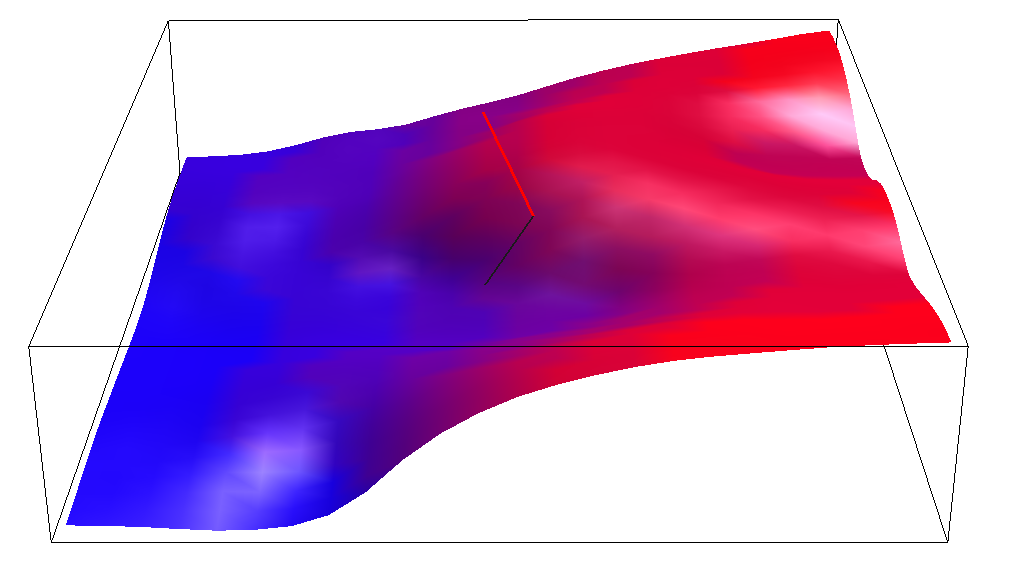
\includegraphics[width=7cm]{erp_ug_3D.png}
\caption{The red line indicates the 3D geopotential direction of the given grid-point according to the surrounding field. Red indicates high values in data, blue low ones.}
\label{fig:erpicum01}
\end{figure}
%
Now the classification can be done. Therefore it is counted, how often one day's similarity-index raises a given threshold (usually between 1 and 0). The day which reaches the highest amount of similar patterns will be the reference of the first type. All days that once are assigned to a type's reference pattern won't be considered further. The following types are determined recursively, one by one using only the remaining ergo unclassified days of all the preceding types.\\

\begin{lstlisting}
Tab. 1:
   cl       ic      obs    count
    1  1.00000        1        1
    2  1.00000        1        1
    3  1.00000        1        1
    4  1.00000        1        1
    5  1.00000        1        1
    6  1.00000        1        1
    7  1.00000        1        1
    8  1.00000        1        1
    9  1.00000        1        1
                           16435 missing!
  ...
   cl       ic      obs    count
    1  0.63000     3809    16392
    2  0.63000     1940       18
    3  0.63000    14423       18
    4  0.63000     1628        5
    5  0.63000     5252        3
    6  0.63000        1        1
    7  0.63000        1        1
    8  0.63000        1        1
    9  0.63000        1        1
                               0 missing!


Tab. 2:
   cl       ic      obs    count
    1  1.00000        1        1
    2  0.99000        1        1
    3  0.98000        1        1
    4  0.97000        1        1
    5  0.96000     1399        3
    6  0.95000    15704       16
    7  0.94000     9148       87
    8  0.93000     4009      280
    9  0.92000    11333      659
                           15390 missing!
  ...
   cl       ic      obs    count
    1  0.70000    12815    16093
    2  0.69000     9232      141
    3  0.68000     3521      111
    4  0.67000     7468       57
    5  0.66000     3780       24
    6  0.65000     7151        5
    7  0.64000     7769        3
    8  0.63000        1        1
    9  0.62000        1        1
                               0 missing!

Tab. 3:
   cl       ic      obs    count
    1  1.00000        1        1
    2  0.95000    15704       16
    3  0.90000    11333     2498
    4  0.85000    14935     5069
    5  0.80000     3431     4559
    6  0.75000     7323     2602
    7  0.70000    10059     1103
    8  0.65000    12865      464
    9  0.60000     7407       88
                              36 missing!
  ...
   cl       ic      obs    count
    1  0.91000    11333     1523
    2  0.86000     6594     5218
    3  0.81000     1157     4391
    4  0.76000     7976     3509
    5  0.71000    10059     1127
    6  0.66000    10710      456
    7  0.61000     7408      155
    8  0.56000    13201       48
    9  0.51000     1191        9
                               0 missing!
\end{lstlisting}

For optimization, the threshold will generally be decreased until all days are classified (starting off with 1, only a few days get classified) (see Tab. 1). Furthermore the threshold is lowered with the type, so let it be 0.70 for the first one, it could be 0.69 for the second (see Tab. 2). In conclusion, several runs are done, gradually increasing the spacing of the thresholds, according to their types (compare Tab. 2 and 3). That is, for the first run there generally are the same thresholds (e.g. 0.63; Tab. 1) for all of the types. For the second run there may be 0.70, 0.69, 0.68, etc. for the first, second, third, etc. type respectively (Tab. 2). Following this for the third run there could be 0.75, 0.73, 0.71, etc., and so on.\\
%
\begin{figure}[h]
\centering
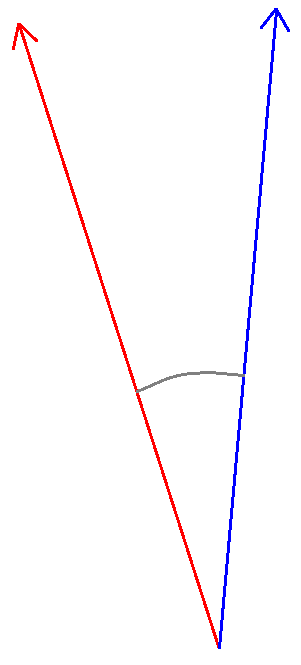
\includegraphics[width=2cm]{erp_ug_arrow.png}
\caption{For a given grid point, the difference between two time steps is calculated from the cosine of the angle between the particular 3D geopotential directions.}
\label{fig:erpicum02}
\end{figure}
%
All the resulting time series of types (one series for each run - or overall-decrement of the threshold) are now evaluated due to their explained cluster variance in the source-data. Only the series which achieves the highest score is returned.

\subsubsection*{Options}
Strictly necessary options:
\begin{itemize}
 \item \verb+-dat <specification>+:\\ Input data. Grid description is necessary!
\end{itemize}
The following options define the classification:
\begin{itemize}
 \item \verb+-ncl <int>+:\\ Determine the number of classes. Default is 9.
 \item \verb+-nrun <real>+:\\ Number of optimization runs. Default is 10000.
\end{itemize}
Options for data output:
\begin{itemize}
 \item \verb+-cla <filename>+:\\ Output file name for the classification catalog.
 \item \verb+-dcol <int>+:\\ Number of date columns in the classification catalog.
 \item \verb+-cnt <filename>+:\\ Output file name for the class centroids.
\end{itemize}

\subsubsection*{Output}
This method returns one file containing the classification catalog. 
Overall class centroids and centroids for each input data set are optional.

\subsubsection*{Examples}
An example with default values:
\begin{lstlisting}
cost733class /*-dat/* /+pth:/+hgt500.dat /+fmt:/+ascii /+lon:/+-37:56:3 /+lat:/+30:76:2 /--met/- ERP /--ncl/- 9  
\end{lstlisting}


%%%%%%%%%%%%%%%%%%%%%%%%%%%%%%%%%%%%%%%%%%%%%%%%%%%%%%%%%%%%%%%%%%%%%%%%
\section{HCL | hclust - Hierarchical Cluster analysis}
\label{hcl}

Hierarchical cluster analysis can be realized in two opposite ways. The first,
divisive clustering, splits up the whole sample, according to some criterion,
into two classes in the first step. On a second hierarchy level it splits up 
one of these classes again into two groups and so. The opposite way is the 
agglomerative clustering: each single observation is treated as a single cluster
and on each hierarchy level of the process the two nearest clusters are merged
to build a new common cluster. In \verb+cost733class+ the agglomerative method is 
implemented.\\
The routine for agglomerative hierarchical clustering offers various criteria for
deciding which clusters should be merged (see below).

\subsubsection*{Options}
Strictly necessary options:
\begin{itemize}
 \item \verb+-dat <specification>+:\\ Input data. No grid description is necessary.
\end{itemize}
The following options define the classification:
\begin{itemize}
 \item \verb+-ncl <int>+:\\ Determine the number of classes. Default is 9.
 \item \verb+-crit <int>+:\\ Criterion for deciding which clusters should be merged. \verb+<int>+ may be:
 \begin{itemize}
  \item[1]: Ward's minimum variance method (default)
  \item[2]: single linkage
  \item[3]: complete linkage
  \item[4]: average linkage
  \item[5]: Mc Quitty's method
  \item[6]: median (Gower's) method
  \item[7]: centroid method
 \end{itemize}
\end{itemize}
Options for data output:
\begin{itemize}
 \item \verb+-cla <filename>+:\\ Output file name for the classification catalog.
 \item \verb+-dcol <int>+:\\ Number of date columns in the classification catalog.
 \item \verb+-cnt <filename>+:\\ Output file name for the class centroids.
\end{itemize}

\subsubsection*{Output}
This method returns one file containing the classification catalog. 
Overall class centroids and centroids for each input data set are optional.

\subsubsection*{Examples}
An example with default values:
\begin{lstlisting}
cost733class /*-dat/* /+pth:/+hgt500.dat /--met/- HCL /--crit/- 1 /--ncl/- 9  
\end{lstlisting}


%%%%%%%%%%%%%%%%%%%%%%%%%%%%%%%%%%%%%%%%%%%%%%%%%%%%%%%%%%%%%%%%%%%%%%%%
\section{Optimization algorithms}

%%%%%%%%%%%%%%%%%%%%%%%%%%%%%%%%%%%%%%%%%%%%%%%%%%%%%%%%%%%%%%%%%%%%%%%%
\subsection{KMN | kmeans - conventional k-means with random seeds}
\label{kmeans}

The $k-means$ algorithm for non-hierarchical cluster analysis works rather simple.
$k$ represents the number of clusters (types or classes) which should be derived. 
This number has to be decided by the user. There is no routine to determine an 
appropriate number automatically.
$means$ denotes the average of each type, which is called centroid in cluster analysis
and plays a fundamental role for this algorithm.
It begins with a so called starting partition. In case of the \verb+kmeans+ implementation
this starting partition is determined by random, i.e. each object is assigned to a cluster
by random. Starting from this (undesirable) state of partitioning, the centroids are calculated
as the average of all objects (e.g. daily pressure fields) within each cluster.
The rest of the process is organized in iterations. In each iteration each object is checked
for being in the cluster with the most similar cluster centroid. Similarity is defined to be the 
Euclidean distance between the centroid and the object in question, but other distance metrics may be used as well. If there is a centroid being
more similar than the one of the current cluster, the object is shifted and the centroids of
the old cluster and of the new cluster are updated (the average is recalculated) in order
to reflect the change in the membership. This means that some of the objects which have been
checked before could be now in the wrong cluster, since its centroid has changed. Therefore
all objects have to be checked again in the next iteration. This process keeps going on
until no shifts occur and all objects are in the cluster with the most similar centroid.
In this case the optimization process has converged to an optimized partition or in other words
to an optimum of the distance minimization function.\\
Due to the existence of local optima in the minimization function (reducing the within-cluster 
variance) for different random starting partitions, different solutions (optimized partitions)
may occur. Therefore the KMN routine runs 10 times by default and selects the best solution in
terms of explained cluster variance (ECV). For better results it is advised to set \verb+-nrun <int>+ to higher values, e.g. 100 or 1000.\\
The standard output of KMN shows the run-number, the number of iterations needed to converge, the explained cluster variance, the sum of within-type variances and the cluster sizes. Eventually it is reported that there are "empty clusters". This can happen during the optimization process and stops this run. However, as many runs as needed to
reach the given run number are triggered.

\subsubsection*{Options}
Strictly necessary options:
\begin{itemize}
 \item \verb+-dat <specification>+:\\ Input data. No grid description is necessary.
\end{itemize}
The following options define the classification:
\begin{itemize}
 \item \verb+-ncl <int>+:\\ Determine the number of classes. Default is 9.
 \item \verb+-nrun <int>+:\\ The number of runs (see above). Default is 10.
 \item \verb+-dist <int>+:\\ Distance metric used for similarity. Default is Euclidean distance (2).
 \item \verb+-crit <int>+:\\ Switch for deciding which algorithm should be used. \verb+<int>+ can be:
 \begin{itemize}
  \item[1]: Optimized algorithm. Default.
  \item[2]: Original algorithm by \citet{Hartigan1979}.
 \end{itemize}
\end{itemize}
Options for data output:
\begin{itemize}
 \item \verb+-cla <filename>+:\\ Output file name for the classification catalog.
 \item \verb+-dcol <int>+:\\ Number of date columns in the classification catalog.
 \item \verb+-cnt <filename>+:\\ Output file name for the class centroids.
\end{itemize}

\subsubsection*{Output}
This method returns one file containing the classification catalog. 
Overall class centroids and centroids for each input data set are optional.

\subsubsection*{Examples}
An example with default values:
\begin{lstlisting}
cost733class /*-dat/* /+pth:/+test.dat /+lon:/+3:20:1 /+lat:/+41:52:1 /--met/- KMN /--nrun 10/- /--ncl/- 9
\end{lstlisting}
Another example using the original algorithm by \citet{Hartigan1979} with 1000 runs and a different number of classes:
\begin{lstlisting}
cost733class /*-dat/* /+pth:/+test.dat /+lon:/+3:20:1 /+lat:/+41:52:1 /--met/- KMN /--nrun 1000/- /--ncl/- 18 /--crit/- 2
\end{lstlisting}

%%%%%%%%%%%%%%%%%%%%%%%%%%%%%%%%%%%%%%%%%%%%%%%%%%%%%%%%%%%%%%%%%%%%%%%%%
%%--> NOTE: CAP is not a subroutine anymore, since it can be produced by data-preprocessing (pca,fil) HCL and KMN
\subsection{CAP | pcaca - k-means of time filtered PC-scores and HCL starting partition}
Actually this classification scheme is not a method on its own, but a combination of two methods and certain data preprocessing steps. This is the reason why there is no argument \verb+-met CAP+ provided or allowed. Instead this classification can be obtained by first running a hierarchical cluster analysis (\verb+-met HCL+) followed by a k-means cluster analysis (\verb+-met KMN+), the latter using the catalog of the former as starting partition.\\
However, since this classification procedure was used in COST Action 733 as a method on its own, it is described in the following:
It is a two-stage procedure which comprises a Principal Component Analysis to derive the dominant patterns of variability and a clustering procedure to classify time series of the principal components \citep{Comrie1996,Ekstrom2002}. \\
If to analyze the entire year is considered (not splitting the data in seasons) raw data fields can be submitted to a temporal filtering to remove variability on time scales longer than the typical duration of regional weather systems but retaining the spatial patterns; otherwise the PCA can be strongly influenced by seasonal variability in the pressure data. Such temporal variability is commonly removed following a method outlined in \cite{Hewitson1992}. Instead of a running mean, however, the \verb+cost733class+ software can be used to apply a gaussian filter. Literature shows that different length filters have been used (from 8 to 13 days for running means corresponding with a length of 31 days for gaussian filters), depending on the area of analysis. To accomplish, the average value of the map on each time step is first calculated, and then an n-days moving average is obtained. Finally, the difference between the original grid values and the filtered average time series values is then obtained, transforming the raw data at each grid point on departures from the smoothed n-days map mean, which are used in all the subsequent analyzes.\\
PCA is used to reduce the original data (usually a large dimension database) into a small set of new variables (principal components) that explain most of the original variability, while the contribution from small-scale variability and noise is ignored. \\
%A correlation matrix must be applied to prevent the possible dominance of the principal components by the grid points with the largest variances, the number of PCs retained being decided by the combination of the most common tests (Scree test, the North rule of thumb, N rule, Kaiser's rule, etc.). Next, 
The retained components were rotated using a VARIMAX procedure to facilitate the spatial interpretation of the principal components and to avoid well-known problems due to the orthogonality constraint of the eigenvector model.\\
%%\begin{figure}
%%\centering
%%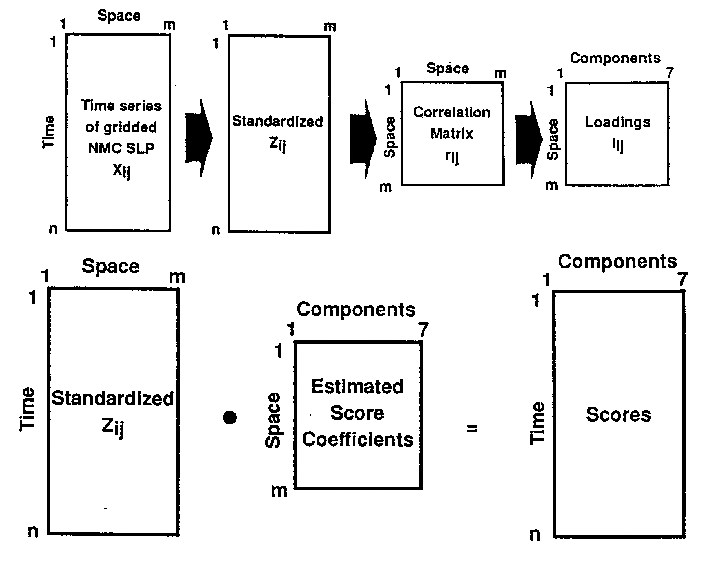
\includegraphics[width=12cm]{cap01.png}
%%\caption{General process to obtain the PC scores in a S-mode PCA}
%%\label{fig:cap01}
%%\end{figure}
%%Unlike T-mode decomposition, S-mode rotated PCs do not represent actual maps; instead, they depict modes of variation in the atmospheric field and can be spatially mapped to delineate areas of homogenous behaviour that portray high frequency atmospheric systems (anticyclones and disturbances). 
%%\begin{figure}
%%\centering
%%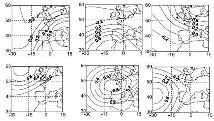
\includegraphics[width=12cm]{cap02.png}
%%\caption{Modes of variability (loadings) extracted from an S-mode PCA}
%%\label{fig:cap02}
%%\end{figure}
Actual maps mix those modes of variability, whose intensity, expressed by the weights of the component scores, varies from time step to time step. Thus, it is necessary to apply a clustering procedure to identify the most common combinations. First, the initial number of clusters and the mean conditions within each cluster (mean scores) are determined by Ward's hierarchical algorithm. Later, those initial clusters are used as seeds to obtain the final solution through a K-means agglomerative algorithm.\\
%A critical step is to determine when the hierarchical procedure must be stopped and select the optimal number of clusters. 
%The "most" parsimonious solution can be obtained using statistics provided by some packages (e.g. R2, Pseudo F, Pseudo t2).
In terms of \verb+cost733class+ command line arguments this method can be realized by the following two commands, the first providing the hierarchical starting partition of the preprocessed data, the second to apply k-means to that starting partition.\\

\subsubsection*{Options}
This is not a subroutine on it own but a combination of two subsequent \verb+cost733class+ runs. Please refer to sections \ref{hcl} and \ref{kmeans}.

\subsubsection*{Output}
This is not a subroutine on it own but a combination of two subsequent \verb+cost733class+ runs. Please refer to sections \ref{hcl} and \ref{kmeans}.

\subsubsection*{Examples}
At first we provide a starting partition by hierarchical cluster analysis of low-pass-filtered PC-scores:
\begin{lstlisting}
cost733class /*-dat/* /+pth:/+slp.dat /+lon:/+-10:30:2.5 /+lat:/+35:60:2.5 /+fdt:/+2000:1:1 /+ldt:/+2008:12:31 /+ddt:/+1d /+nrm:/+1 /+fil:/+31 /*-pcw/* 0.9 /--met/- HCL /--ncl/- 10
\end{lstlisting}
Then we run \verb+cost733class+ with k-means using the starting partition created above:
\begin{lstlisting}
cost733class /*-dat/* /+pth:/+slp.dat /+lon:/+-10:30:2.5 /+lat:/+35:60:2.5 /+fdt:/+2000:1:1 /+ldt:/+2008:12:31 /+ddt:/+1d /+nrm:/+1 /+fil:/+31 /*-pcw/* 0.9 /*-clain/* /+pth:/+HCL10.cla /+dtc:/+3 /--met/- KMN /--ncl/- 10
\end{lstlisting}

%%%%%%%%%%%%%%%%%%%%%%%%%%%%%%%%%%%%%%%%%%%%%%%%%%%%%%%%%%%%%%%%%%%%%%%%
\subsection{CKM | ckmeans - k-means with dissimilar seeds}

In this classification, a modified minimum distance method is used for producing the seeds for 
k-means clustering. According to the concept of optimum complexity which is applied to the gain 
in explained variance with growing number of classes the authors of this method suggest a
number of around 10 clusters \citep{Enke1997}. The following steps are performed:
\begin{itemize}
\item The initialization takes place by randomly selecting one weather situation (object).
\item In a stepwise procedure the starting partition, consisting of the ten most dissimilar 
weather situations (days) is gradually identified, see Fig.~\ref{fig:ckmean01}. 
Similarity and dissimilarity are being 
defined by a variant of the euclidean distance measure RMSD. 
%
\begin{equation}
\label{equaRMSD}
 RMSD=\sqrt{\frac{1}{n}\sum^{n}_{i=1}R^{2}_{i} }
\end{equation}
%
\noindent With $R_i =$: Difference between class centroid value and current day value;  $n =$: Number of grid points.
If more than one atmospheric field is used, 
a normalization is necessary to maintain comparability and to retain the additive nature 
of the distances \citep[for more details see]{Enke2005a}.

\item All remaining days of the archive are assigned to their most similar class. 
With each day entering a class, a position shift takes place which in turn makes it necessary to re-compute 
the centroid positions. As a consequence, the multi-dimensional distance between class centroids continually 
decreases (see Fig. \ref{fig:ckmean}); the variability within the individual classes, on the other hand, increases. 
\item After the assignment of all days has been performed and an intermediate stage has been reached, 
an iterative process is launched. With each pass, members of the clusters are exchanged in order to improve 
the separation of the classes and their compactness. Gradually, a final centroid configuration emerges. 
In order to retain representative results, classes are kept in the process only if they do not fall short of 
a certain number, e.g., 5\% of all days. Otherwise the class will be removed and its contents distributed 
among the remaining classes. The iterative process will be stopped if two successive iterations leaves the 
contents of the classes unchanged.
\end{itemize}
%
\begin{figure}[h]
\centering
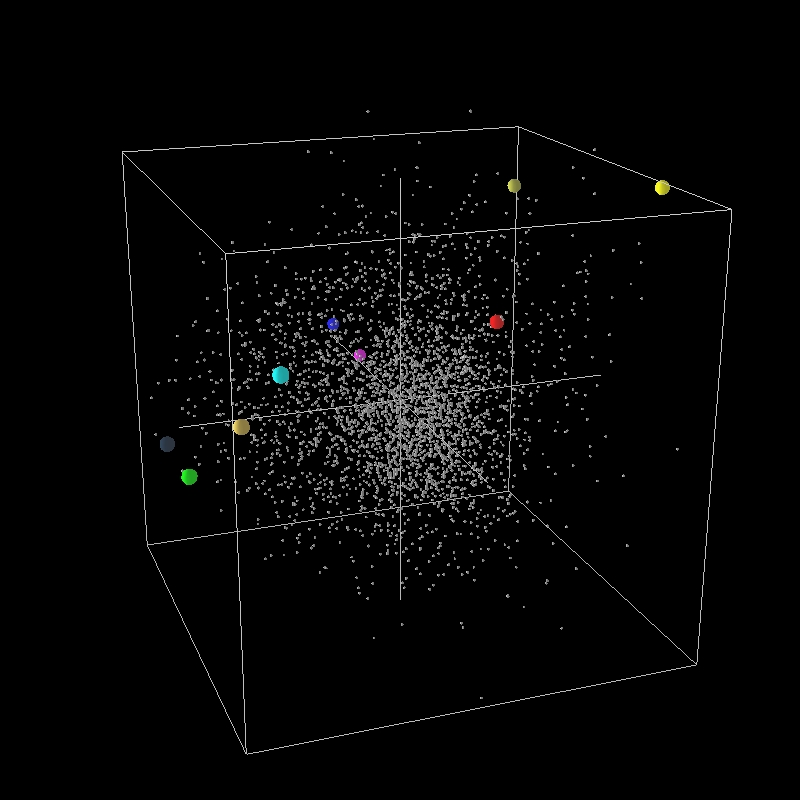
\includegraphics[width=8cm]{ckm01.png}
\caption{Starting seed points for CKM classification method using the example data set slp.dat and 9 classes.
The projection of each daily pattern into the three-dimensional PCA phase space is shown by small spheres. Large spheres represent the projected centroids. ---> link to command line + revert black background }
\label{fig:ckmean01}
\end{figure}
%
The centroids converge towards a final configuration which has no similarity with the starting partition. 
The process is sketched in Fig.~\ref{fig:ckmean} \citep[from][]{Enke1997}. Beginning with the initial conditions 
(denoted 'a'), the intermediate stage (denoted 'b') is reached which is characterized on the one hand by a 
higher proximity of the classes but on the other hand by large 'class volumes' (i.e., high within-type variability) 
since the assignment of days is not optimized. After the iterative exchange process, the final stage (denoted 'c') 
is free of overlap (i.e., it is well separated, exhibiting high between-type variability) and consists of comparably 
compact classes (i.e., it exhibits low within-type variability), see Fig.~\ref{fig:ckmean02}.\\
%
\begin{figure}[h]
\centering
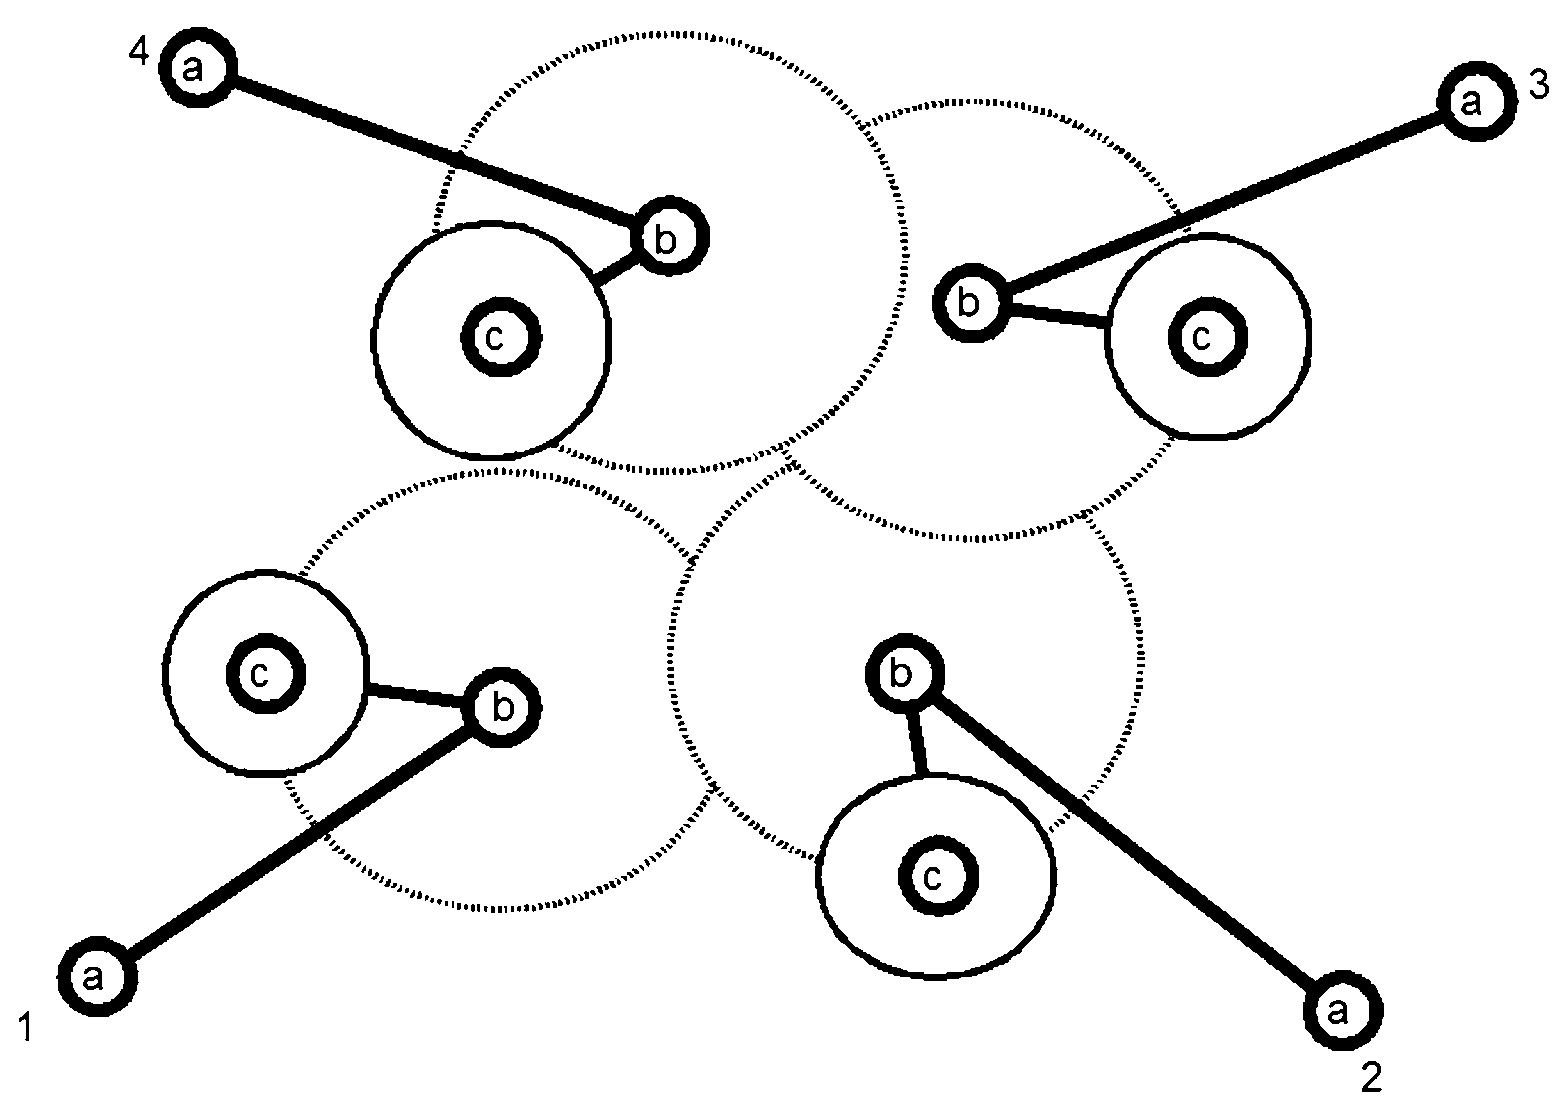
\includegraphics[width=8cm]{ckmeans_diagram.png}
\caption{Sketch of the iterative process for ckmeans that leads from the starting partition to the final stage. For details see main text.}
\label{fig:ckmean}
\end{figure}
%
\subsubsection*{Options}
Strictly necessary options:
\begin{itemize}
 \item \verb+-dat <specification>+:\\ Input data. No grid description is necessary.
\end{itemize}
The following options define the classification:
\begin{itemize}
 \item \verb+-ncl <int>+:\\ Determine the number of classes. Default is 9.
\end{itemize}
Options for data output:
\begin{itemize}
 \item \verb+-cla <filename>+:\\ Output file name for the classification catalog.
 \item \verb+-dcol <int>+:\\ Number of date columns in the classification catalog.
 \item \verb+-cnt <filename>+:\\ Output file name for the class centroids.
\end{itemize}
%
\begin{figure}[h]
\centering
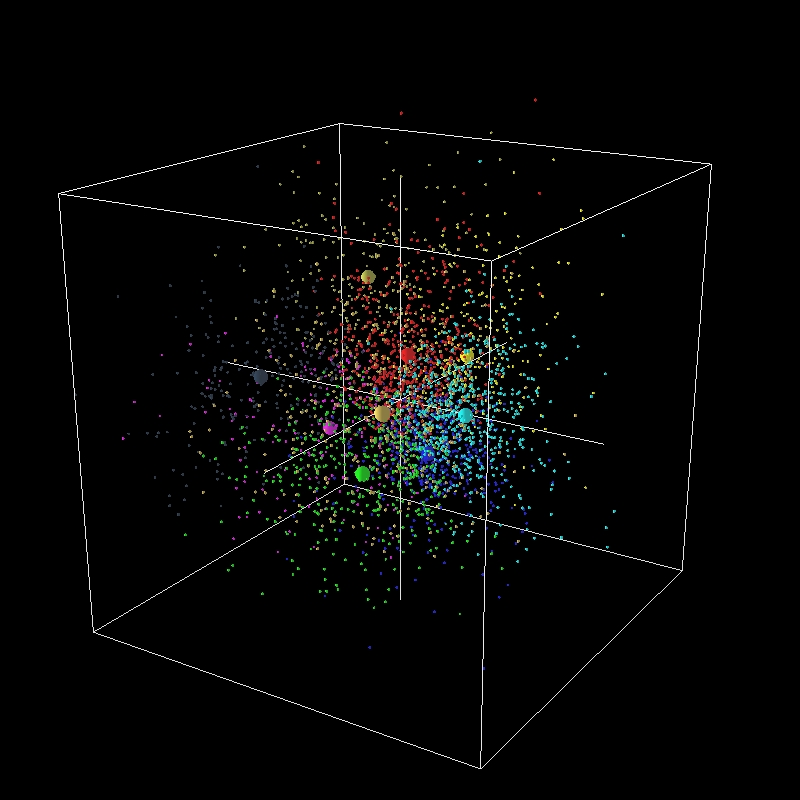
\includegraphics[width=8cm]{ckm02.png}
\caption{Final partition for CKM classification method using the example data set slp.dat and 9 classes. 
The projection of each daily pattern into the three-dimensional PCA phase space is shown by small spheres. Large spheres represent the projected centroids.}
\label{fig:ckmean02}
\end{figure}
%
\subsubsection*{Output}
This method returns one file containing the classification catalog. 
Overall class centroids and centroids for each input data set are optional.

\subsubsection*{Examples}
An example with default values:
\begin{lstlisting}
cost733class /*-dat/* /+pth:/+test.dat /+lon:/+3:20:1 /+lat:/+41:52:1 /--met/- CKM /--ncl/- 9
\end{lstlisting}

%%%%%%%%%%%%%%%%%%%%%%%%%%%%%%%%%%%%%%%%%%%%%%%%%%%%%%%%%%%%%%%%%%%%%%%%
\subsection{DKM | dkmeans - a variant of ckmeans}

DKM differs from CKM in three points:

\begin{enumerate}
\item For finding dissimilar seed patterns for the 2nd and further clusters 
not only the sum of the distances to the preceding seeds is used but the minimum
of these distances is maximized.
\item There is no 5\% minimum frequency limit for keeping all clusters. In most cases if the population temporarily decreases below 5\% of the total sample size, it is filled up again later during the iterations.
\item Furthermore it is possible to select a number of runs. As the initiation of the starting partition partially follows random assignment, results differ from run to run. Therefore the solution with highest explained cluster variance will be chosen.
\end{enumerate}

\subsubsection*{Options}
Strictly necessary options:
\begin{itemize}
 \item \verb+-dat <specification>+:\\ Input data. No grid description is necessary.
\end{itemize}
The following options define the classification:
\begin{itemize}
 \item \verb+-ncl <int>+:\\ Determine the number of classes. Default is 9.
 \item \verb+-nrun <int>+:\\ The number of runs (see above). Default is 10.
 \item \verb+-crit <int>+:\\ Switch for choosing the method for initial pattern selection . \verb+<int>+ can be:
 \begin{itemize}
  \item[1]: Choose the observation which minimizes the distance to the total centroid.
  \item[2]: Choose the observation which maximizes the distance to the total centroid.
  \item[3]: Randomly choose a observation. Default.
 \end{itemize}
\end{itemize}
Options for data output:
\begin{itemize}
 \item \verb+-cla <filename>+:\\ Output file name for the classification catalog.
 \item \verb+-dcol <int>+:\\ Number of date columns in the classification catalog.
 \item \verb+-cnt <filename>+:\\ Output file name for the class centroids.
\end{itemize}

\subsubsection*{Output}
This method returns one file containing the classification catalog. 
Overall class centroids and centroids for each input data set are optional.

\subsubsection*{Examples}
An example with default values:
\begin{lstlisting}
cost733class /*-dat/* /+pth:/+test.dat /+lon:/+3:20:1 /+lat:/+41:52:1 /--met/- DKM /--ncl/- 9 /--nrun/- 10 /--crit/- 3
\end{lstlisting}
%%%%%%%%%%%%%%%%%%%%%%%%%%%%%%%%%%%%%%%%%%%%%%%%%%%%%%%%%%%%%%%%%%%%%%%%
\subsection{PXK | pcaxtrkm - k-means using PXE starting partitions}

This method follows the application of PXE but differs in so far that the final CTs are established using the iterative clustering method (K-means). In this way, for the optimization of the final clusters, the K-means method starts using the centroids obtained with the" extreme scores" criteria as starting partitions.

\subsubsection*{Options}
Strictly necessary options:
\begin{itemize}
 \item \verb+-dat <specification>+:\\ Input data. No grid description is necessary.
\end{itemize}
The following options define the classification:
\begin{itemize}
 \item \verb+-ncl <int>+:\\ Determine the number of classes.  Always has to be a pair value / even number (2, 4, 8, 10,...) Default is 8.
\item \verb+-niter <int>+:\\ Maximum number of iterations. Leave it unchanged for PXK in order to reach convergence (default: \verb+-niter 9999999+), i.e. this option should be omitted for PXK. 
\item \verb+-crit <int>+:\\ Normalization method of the input data before the PCA is performed: . \verb+<int>+ can be:
 \begin{itemize}
  \item[0]: Only normalize patterns for PCA (original).
  \item[1]: Normalize patterns and normalize grid point values afterwards.
  \item[2]: Normalize patterns and center grid point values afterwards (default).
 \end{itemize}
The thresholds for definition of extreme score cases can be changed by:
\item \verb+-thres <real>+: \\
	Threshold defining key group (default is 2.0).
\item \verb+-delta <real>+: \\
	Score limit for other PCs to define uniquely leading PC (default is 1.0).
\end{itemize}
Options for data output:
\begin{itemize}
 \item \verb+-cla <filename>+:\\ Output file name for the classification catalog.
 \item \verb+-dcol <int>+:\\ Number of date columns in the classification catalog.
 \item \verb+-cnt <filename>+:\\ Output file name for the class centroids.
 \item \verb+-idx <basename>+:\\ Output base name for rotated scores (*.sco).
\end{itemize}

\subsubsection*{Output}
This method returns one file containing the classification catalog. 
Overall class centroids and centroids for each input data set as well as a file containing the rotated scores are optional.

\subsubsection*{Examples}
An example with default values:
\begin{lstlisting}
cost733class /*-dat/* /+pth:/+test.dat /--met/- PXK /--ncl/- 8 /--niter/- 9999999 /--crit/- 2 /--thres/- 2.0 /--delta/- 1.0
\end{lstlisting}
%%%%%%%%%%%%%%%%%%%%%%%%%%%%%%%%%%%%%%%%%%%%%%%%%%%%%%%%%%%%%%%%%%%%%%%%
\subsection{SAN | sandra - simulated annealing and diversified randomization}
SANDRA means Simulated ANealing and Diversified RAndomization. Essentially it is a non-hierarchical cluster
analysis method like k-means. However, it usually finds better solutions than conventional k-means. 

\subsubsection*{Options}
Strictly necessary options:
\begin{itemize}
 \item \verb+-dat <specification>+:\\ Input data. No grid description is necessary.
\end{itemize}
The following options define the classification:
\begin{itemize}
 \item \verb+-ncl <int>+:\\ 
 Determine the number of classes. Default is 9. 
 \item \verb+-nrun <int>+:\\ 	
 The number of diversified runs for searching the best result.
 Note that if compilation has been started using the \verb+-openmp+ option 
 (i.e. \verb+.\configure CC=icc FC=ifort FCFLAGS="-openmp"+) the runs are executed in parallel.
 How many parallel threads are used might depend on a environment variable (e.g. \verb+NTHREAD=4+)
 of your operating system. For details check the documentation of your compiler. Default is 1000. Note that this may cause very long runtimes and is no bug.
 \item \verb+-niter <int>+:\\ Maximum number of iterations. Leave it unchanged in order to reach convergence (default: infinity). Sometimes SAN ends up in an endless loop. Then set set it to a finite value, i. e. \verb+-niter 10000+. However, this is very unlikely.
\item \verb+-cool <real>+:\\
This parameter controls the speed of cooling down the temperature parameter (i.e. how fast
the probability for so called wrong shifts of objects is reduced). The higher \verb+<real>+, the slower the decrease. Note that it must be less than one (e.g. 0.999), else the routine will never stop. Default is 0.99.
\end{itemize}
Options for data output:
\begin{itemize}
 \item \verb+-cla <filename>+:\\ Output file name for the classification catalog.
 \item \verb+-dcol <int>+:\\ Number of date columns in the classification catalog.
 \item \verb+-cnt <filename>+:\\ Output file name for the class centroids.
\end{itemize}

\subsubsection*{Output}
This method returns one file containing the classification catalog. 
Overall class centroids and centroids for each input data set are optional.

\subsubsection*{Examples}
An example with default values:
\begin{lstlisting}
cost733class /*-dat/* /+pth:/+test.dat /--met/- SAN /--ncl/- 9 /--nrun/- 1000 /--cool/- 0.99
\end{lstlisting}

%%%%%%%%%%%%%%%%%%%%%%%%%%%%%%%%%%%%%%%%%%%%%%%%%%%%%%%%%%%%%%%%%%%%%%%%
% Unable to find this routine in code. Where is it?
%\subsection{SAT | sandrat - time constrained simulated annealing and diversified randomization}
%
%Time constraint clustering \citep{Jolliffe2010} is a variant of non-hierarchical cluster analysis which accounts for the distance in time
%between two objects and not only for their similarity. The Euclidean distance is therefore weighted by a factor reducing
%the dissimilarity between two patterns if they are close together on the time axis. The impact of this weight can be
%controlled by \verb+-lambda <real>+. High values of \verb+lambda+ cause temporally neighboring patterns to be classified 
%into the same cluster more easily.
%The weighting has been implemented into the SANDRA method. Thus all options of this method (see above) apply also here.

%%%%%%%%%%%%%%%%%%%%%%%%%%%%%%%%%%%%%%%%%%%%%%%%%%%%%%%%%%%%%%%%%%%%%%%%
\subsection{SOM | som - self organizing (feature) maps (neural network according to Kohonen)}

Self organizing maps describe a way to arrange types defined by their features (grid point values) in a structure
where similar types are adjacent to each other (a map). This structure commonly is a two dimensional matrix describing
a network of neurons (i.e. types) which are connected to their neighbors in the four directions. 
However this structure can also be a one dimensional arrangement where the neurons are connected to their left and right
neighbors only, which is the case for the method implemented in \verb+cost733class+. \\
The number of neurons is given by the number of types provided by the \verb+-ncl <int>+ option. Each neuron has as many features
as there are grid points or variables in the input data set (columns in case of ASCII-input). The values of each neuron are initialized 
by random numbers. Then for each iteration the data of the objects to classify are presented one after the other to these neurons and
in each case a winner neuron is determined by the minimum Euclidean distance between the presented object and the neurons. The winner neuron and
its neighbors are then modified to become more similar to the presented object by calculating the weighted mean between the old neuron 
values and the object, where the weight is a tuning parameter called \verb+alpha+. How many neighbors of the winner neuron
are affected of this modification of the neuron values depends on the \verb+radius+-parameter. At the beginning of the classification process
it is large, thus all neurons are affected, but it is slowly reduced so that at the end only the winner neuron will be modified. Also the weight
\verb+alpha+ is slowly modified during the iterations (training epochs) thus at the end the object (pattern) which is assigned to the winner
neuron has a large impact on the modification of the neuron values.
If the neuron values do not change any more (convergence) the process is finished and each object is assigned to the most similar neuron (type).

\subsubsection*{Options}
Strictly necessary options:
\begin{itemize}
 \item \verb+-dat <specification>+:\\ Input data. No grid description is necessary.
\end{itemize}
The following options define the classification:
\begin{itemize}
 \item \verb+-ncl <int>+:\\ 
 Determine the number of neurons/classes. Default is 9.  
 \item \verb+-nrun <int>+:\\ 	
 The number of diversified runs for searching the best result. Note that if compilation has been started using the \verb+-openmp+ option 
 (i.e. \verb+.\configure CC=icc FC=ifort FCFLAGS="-openmp"+) the runs are executed in parallel.
 How many parallel threads are used might depend on a environment variable (e.g. \verb+NTHREAD=4+)
 of your operating system. For details check the documentation of your compiler. Default is 10.
% \item \verb+-crit <int>+:\\ Default is 1.
 \item \verb+-cool <real>+:\\ Factor for reduction of learning rate. Default is 0.99.
%??? \item \verb+-step <int>+:\\  Default is 100.
 \item \verb+-niter <int>+\\ Number of iterations (training epochs). Default is 10000. 
\end{itemize}
Options for data output:
\begin{itemize}
 \item \verb+-cla <filename>+:\\ Output file name for the classification catalog.
 \item \verb+-dcol <int>+:\\ Number of date columns in the classification catalog.
 \item \verb+-cnt <filename>+:\\ Output file name for the class centroids.
\end{itemize}

\subsubsection*{Output}
This method returns one file containing the classification catalog. 
Overall class centroids and centroids for each input data set are optional.

\subsubsection*{Examples}
An example with default values:
\begin{lstlisting}
cost733class /*-dat/* /+pth:/+test.dat /--met/- SOM /--ncl/- 9 /--nrun/- 10 /--niter/- 10000 /--cool/- 0.99 
\end{lstlisting}

%%%%%%%%%%%%%%%%%%%%%%%%%%%%%%%%%%%%%%%%%%%%%%%%%%%%%%%%%%%%%%%%%%%%%%%%
\subsection{KMD | kmedoids - partitioning around medoids}

K-medoids is similar to k-means as it iteratively minimizes a cost function (within cluster variability). 
However it differs, as it does not use the cluster mean (i.e. centroids) for measurement of within-type 
variability but uses given data points as centers of the clusters. The algorithm consists of the following steps:
\begin{enumerate}
\item select k objects by random to be the initial cluster centers, i.e. medoids.
\item assign all other objects to them according to the minimum distance
\item calculate the cost function, which is the sum of the distances between each object and its nearest medoid
\item begin an iteration
\item for each cluster check all objects whether they would be a better medoid, if yes change the medoid and update the 
assignments and cost function
\item if no enhancement is possible by changing the medoid stop the iterations.
\end{enumerate}

%The following options apply for KMD:
%\begin{itemize}
%\item \verb+-ncl <int>+ the number of clusters
%\item \verb+-crit <int>+ choice of the distance metric: 0=Chebychev, 1=Manhattan, 2=Euclid, int>2=Minkovski distance of order int
%\item \verb+-opengl+ only if compiled with "configure --enable-opengl": activate visualization.
%\item \verb+-gljpeg+ only if compiled with "configure --enable-opengl": create image for each frame.
%\item \verb+-nrun <int>+ number of runs with initial random medoids. The solution with minimum cost function will be chosen. Default for \verb+<int>+ is 10.
%\end{itemize}

\subsubsection*{Options}
Strictly necessary options:
\begin{itemize}
 \item \verb+-dat <specification>+:\\ Input data. No grid description is necessary.
\end{itemize}
The following options define the classification:
\begin{itemize}
 \item \verb+-ncl <int>+:\\ 
 Determine the number of classes. Default is 9.  
 \item \verb+-nrun <int>+:\\ 	
 Number of runs with initial random medoids. The solution with minimum cost function will be chosen. Default for is 10.
 \item \verb+-dist <int>+: \\
 Distance metric used for similarity. Default is Euclidean distance (2).
\end{itemize}
Options for data output:
\begin{itemize}
 \item \verb+-cla <filename>+:\\ Output file name for the classification catalog.
 \item \verb+-dcol <int>+:\\ Number of date columns in the classification catalog.
 \item \verb+-cnt <filename>+:\\ Output file name for the class centroids.
\end{itemize}

\subsubsection*{Output}
This method returns one file containing the classification catalog. 
Overall class centroids and centroids for each input data set are optional.

\subsubsection*{Examples}
An example with default values:
\begin{lstlisting}
cost733class /*-dat/* /+pth:/+test.dat /--met/- KMD /--ncl/- 9 /--nrun/- 10 /--dist/- 2 
\end{lstlisting}

%%%%%%%%%%%%%%%%%%%%%%%%%%%%%%%%%%%%%%%%%%%%%%%%%%%%%%%%%%%%%%%%%%%%%%%%
\section{Random classifications}

%%%%%%%%%%%%%%%%%%%%%%%%%%%%%%%%%%%%%%%%%%%%%%%%%%%%%%%%%%%%%%%%%%%%%%%%
\subsection{RAN | random}
This method does not use any input data but randomly selects any arbitrary number as type number
for each object. The respective number is retrieved from a random number generator between 1 and the 
maximum number of classes given by the \verb+-ncl <integer>+ option.
More than one catalog can be produced by using the \verb+-nrun <int>+ option. By default the best catalog out of these 
according to the explained cluster variance (see \ref{evaluation}) is selected and written to the \verb+-cla+ file. If the option \verb+-mcla <filename>+ is given all catalogs will be written to that file (each catalog one additional column).

\subsubsection*{Options}
Strictly necessary options:
\begin{itemize}
 \item \verb+-dat <specification>+:\\ Input data. No grid description is necessary.
\end{itemize}
The following options define the classification:
\begin{itemize}
 \item \verb+-ncl <int>+:\\ 
 Determine the number of classes. Default is 9.  
 \item \verb+-nrun <int>+:\\ 	
 Number of runs. By default the best solution will be chosen. Default for is 1000.
\end{itemize}
Options for data output:
\begin{itemize}
 \item \verb+-cla <filename>+:\\ Output file name for the catalog with the best classification according to explained cluster variance.
 \item \verb+-mcla <filename>+:\\ Output file name for all classification catalogs.
 \item \verb+-dcol <int>+:\\ Number of date columns in the classification catalog.
 \item \verb+-cnt <filename>+:\\ Output file name for the class centroids.
\end{itemize}

\subsubsection*{Output}
This method returns one file containing the classification catalog. 
Overall class centroids, centroids for each input data set as well as a file containing a catalog for each run are optional.

\subsubsection*{Examples}
An example with default values:
\begin{lstlisting}
cost733class /*-dat/* /+pth:/+test.dat /--met/- RAN /--ncl/- 9 /--nrun/- 1000 
\end{lstlisting}
An example producing an output file with 100 catalogs.
\begin{lstlisting}
cost733class /*-dat/* /+pth:/+test.dat /--met/- RAN /--ncl/- 9 /--nrun/- 100 /--mcla/- RAN9ncl_all.cla
\end{lstlisting}

%%%%%%%%%%%%%%%%%%%%%%%%%%%%%%%%%%%%%%%%%%%%%%%%%%%%%%%%%%%%%%%%%%%%%%%%
\subsection{RAC | randomcent}
In contrast to the method above input data have to be provided for method \verb+RAC+. Any arbitrary 
object of these input data is used as seed or key object (centroid) for each class. All the rest
of the input data are then assigned to these centroids by determination of the minimum Euclidean distance.
If the option \verb+-idx <filename>+ provides a name of an non-existing file, the numbers of the objects used as medoids, which are determined by random, are stored to this file. It has as many rows as there are different classification (\verb+-nrun <integer>+) and as many columns as there are types (\verb+-ncl <integer>+).
If in contrast the file is old and contains at least enough numbers to provide the seeds, these numbers will be used for seeding the types. However they all have to less or equal than the number of objects to be classified. This feature allows for comparable random medoid classifications just differing e.g. by data preprocessing.

\subsubsection*{Options}
Strictly necessary options:
\begin{itemize}
 \item \verb+-dat <specification>+:\\ Input data. No grid description is necessary.
\end{itemize}
Optional data input:
\begin{itemize}
 \item \verb+-idx <filename>+:\\ Input data for seeds.
\end{itemize}
The following options define the classification:
\begin{itemize}
 \item \verb+-ncl <int>+:\\ 
 Determine the number of classes. Default is 9.  
 \item \verb+-nrun <int>+:\\ 	
 Number of runs. By default the best solution will be chosen. Default for is 1000.
\end{itemize}
Options for data output:
\begin{itemize}
 \item \verb+-cla <filename>+:\\ Output file name for the catalog with the best classification according to explained cluster variance.
 \item \verb+-mcla <filename>+:\\ Output file name for all classification catalogs.
 \item \verb+-dcol <int>+:\\ Number of date columns in the classification catalog.
 \item \verb+-idx <basename>+:\\ Output base name for all seeds (*\_med.list). Only if \verb+<filename>+ doesn't exist. Default is OUTPUT.
 \item \verb+-cnt <filename>+:\\ Output file name for the class centroids.
\end{itemize}

\subsubsection*{Output}
This method returns one file containing the classification catalog. 
Overall class centroids, centroids for each input data set as well as a file containing a catalog for each run are optional. Moreover it is possible to obtain a file containing the seeds of initial random assignment.

\subsubsection*{Examples}
An example with default values:
\begin{lstlisting}
cost733class /*-dat/* /+pth:/+test.dat /--met/- RAC /--ncl/- 9 /--nrun/- 1000 /--idx/- OUTPUT_med.list
\end{lstlisting}
An example reading a seed file with 10 different seeds for 9 classes and output of each classification catalog:
\begin{lstlisting}
cost733class /*-dat/* /+pth:/+test.dat /--met/- RAC /--idx/- seed_ncl9_nrun10_med.list /--ncl/- 9 /--nrun/- 10 /--mcla/- RAC9ncl_nrun10_all.cla
\end{lstlisting}
The seed file \verb+seed_ncl9_nrun10_med.list+ could look like this:
\begin{lstlisting}
   1844    553    881   1612   1800   1886   2263   2663    420
    264   1376   2704    568    459   2542     63   2006   2022
   1948   2553     73   1077   2602   1517   2206   1319    479
   1717    145   2614   2030   2518   2510   1045    464   1460
    652   1082   2295   1467   2051     90   2050   1678   2094
   1691    718   1901   1927    165   2368   1634   1211     68
   1787    599    768   1791   2611    702    927    532   1616
    334   1058   1284   2626     52   2424   1122   1995   2576
   1987   1008   2198    487   2595   1380   1687   1736    614
   1753    390    996   1874    956   2519    770   1404    616
\end{lstlisting}
%%%%%%%%%%%%%%%%%%%%%%%%%%%%%%%%%%%%%%%%%%%%%%%%%%%%%%%%%%%%%%%%%%%%%%%%
%%\subsection{RCC | randomcentconst}
%%This methods differs from the \verb+RAC+ method above by using constraints for the choice of the 
%%random centroids. These constraints ensure a minimum distance between the randomly chosen centroids.

%%%%%%%%%%%%%%%%%%%%%%%%%%%%%%%%%%%%%%%%%%%%%%%%%%%%%%%%%%%%%%%%%%%%%%%%
\chapter{Assignments to existing classifications}

%%%%%%%%%%%%%%%%%%%%%%%%%%%%%%%%%%%%%%%%%%%%%%%%%%%%%%%%%%%%%%%%%%%%%%%%
\section{ASC | assign}
\label{asc}
Using this option any data set of the same number of variables as a given centroid file can be assigned 
to the respective classes. For each record (object) of the input data set the dissimilarity/distance between the object 
and the centroids is then calculated and the class number is chosen to be the one with the minimum distance.
%
%The following distance metrics can be selected by the \verb+-dist <int>+ option:
%\begin{itemize}
%\item \verb+int >= 0+: Minkowsky distance of order \verb+<int>+, i.e. 1=Manhattan/block, 2=Euclidean, ..., 0=Chebychev
%\item \verb+int = -1+: inverse Pearson correlation coefficient for non-normalized objects using population dof (n-1)
%\item \verb+int = -2+: inverse Pearson correlation coefficient for non-normalized objects using sample dof (n)
%\item \verb+int = -3+: dist = 1.D0 - sum( vec1*vec2 ) / (nvar-1), where vec1 and vec2 are the objects
%\item \verb+int = -4+: dist = 1.D0 - sum( vec1*vec2 ) / (nvar)
%\end{itemize}
%The default distance = 2 (Euclidean distance).

\subsubsection*{Options}
Strictly necessary options:
\begin{itemize}
 \item \verb+-dat <specification>+:\\ Input data. No grid description is necessary.
 \item \verb+-cntin <filename>+:\\ Input centroid file. Only ASCII is allowed.
\end{itemize}
The following options define the classification:
\begin{itemize}
 \item \verb+-dist <int>+:\\ 
 The distance metric used for measure of similarity between the given centroids and each observation. Default is Euclidean distance (2). 
\end{itemize}
Options for data output:
\begin{itemize}
 \item \verb+-cla <filename>+:\\ Output file name for the catalog with the best classification according to explained cluster variance.
 \item \verb+-dcol <int>+:\\ Number of date columns in the classification catalog.
\end{itemize}

\subsubsection*{Output}
This method returns one file containing the classification catalog. 

\subsubsection*{Examples}
An example with default values:
\begin{lstlisting}
cost733class /*-dat/* /+pth:/+test.dat /--met/- ASC /--dist/- 2 /--cntin/- KMN09ncl.txt
\end{lstlisting}

%%%%%%%%%%%%%%%%%%%%%%%%%%%%%%%%%%%%%%%%%%%%%%%%%%%%%%%%%%%%%%%%%%%%%%%%
\section{CNT | centroid}
This operation allows to create centroids of a given classification catalog using the given data. 
The flag \verb+-clain <spec>+ is  used to provide an existing catalog file comprising the integer class numbers
for each object in each line respectively. In order to calculate the centroids as means of
all objects contained within the respective class the data used for building the centroids has to be 
provided by one or more \verb+-dat <specification>+ arguments. The number of records or lines (e.g. time steps)
in the catalog file has to fit the number of records or lines of the data set.
By providing the \verb+-cnt <filename>+ option the centroids are written to the respective file. 
In a subsequent run of \verb+cost733class+ these centroid data can be used for assigning additional data
to the centroids (see method \verb+ASC+ above) in order to produce a new catalog file.


%%%%%%%%%%%%%%%%%%%%%%%%%%%%%%%%%%%%%%%%%%%%%%%%%%%%%%%%%%%%%%%%%%%%%%%%
\chapter{Evaluation of classifications}
\label{evaluation}
Several statistical metrics characterizing classifications in terms of separability among classes and variability within classes (see e.g.  \citet{Beck2010}) can be applied to existing catalogs (provided by -clain <spec>) and for a given input data set (-dat <specification>).


%%%%%%%%%%%%%%%%%%%%%%%%%%%%%%%%%%%%%%%%%%%%%%%%%%%%%%%%%%%%%%%%%%%%%%%%
\section{EVPF | evpf - explained variation and pseudo F value}

This routine calculates the explained variation (EV) on the basis of the ratio of the sum of Squares within classes/circulation types (WSS) and the total sum of squares (TSS).

\begin{equation}
EV = 1 - \frac{WSS}{TSS}
\end{equation}

Additionally the so called Pseudo-F statistic (PF) according to  \citet{Calinski1974} is calculated as the ratio of the sum of squares between classes (BSS) and the sum of squares within classes (WSS) thereby taking into account the number of cases (n) and classes (k).

\begin{equation}
PF = \frac {BSS / (k-1)}  {WSS / (n-k)}
\end{equation}

Command line parameters relevant for EVPF:
\begin{itemize}
\item \verb+-clain <spec>+:  catalog input, see \ref{clainput}.
\item \verb+-dat <specification>+: input data set to which evaluation metrics are applied
\item \verb+-crit <integer>+: file output for [1] each individual variable and all variables (default) or [2] just the latter.
\item \verb+-idx <character string>+: base string for naming of output file(s)
\end{itemize}

Output:
\begin{itemize}
\item \verb+<-idx>_ev.list, <-idx>_pf.list+: EV- / PF-indices estimated over all variables from the input data set for months, seasons and the whole year (jan, feb, mar, apr, may, jun, jul, aug, sep, oct, nov, dec, win, spr, sum, aut, yea).
\item \verb+<-idx>_ev.fld, <-idx>_pf.fld+: EV- / PF-indices estimated for each indvidual variable from the input data set for months, seasons and the whole year (jan, feb, mar, apr, may, jun, jul, aug, sep, oct, nov, dec, win, spr, sum, aut, yea).
\end{itemize}


%%%%%%%%%%%%%%%%%%%%%%%%%%%%%%%%%%%%%%%%%%%%%%%%%%%%%%%%%%%%%%%%%%%%%%%%
\section{ECV | exvar}

This routine calculates the explained cluster variance (ECV is the same than EV, see above) values for existing catalogs
(provided by \verb+-clain <spec>+) for the given input data set (\verb+-dat <specification>+). 
In contrast to EVPF it does not discern seasons and does not create output files. It just calculates the ECV, 
prints it to the screen and exits.

\begin{equation}
ECV = 1 - \frac{WSS}{TSS}
\end{equation}
, where 
\begin{equation}
WSS = \sum^{k}_{j=1}{ \sum_{i \in C_j}{ {D_{(X_i,\bar{X_j})}}^2} }
\end{equation}
, $C_j$ is the Class $j$ of the $k$ classes, and the squared Euclidean distance between an element and its centroid
\begin{equation}
D_{(X_i,\bar{X}_j)} = \sum^{m}_{l=1}{ (X_{il} - \bar{X}_{jl})^2 }
\end{equation}

$TSS$ is the total sum of squared differences between all elements and the overall centroid (mean):

\begin{equation}
TSS = \sum^{n}_{i=1} \sum^{m}_{l=1} { (X_{il} - \bar{X}_l)^2}
\end{equation}.


The input catalog file can have more than one catalog columns (e.g. as produced by \verb+-met RAC+).
The ECV is calculated for all catalogs within this file one after the other.

%%%%%%%%%%%%%%%%%%%%%%%%%%%%%%%%%%%%%%%%%%%
\section{WSDCIM | wsdcim - Within-type standard deviation and confidence interval of the mean}

The within-type standard deviation (WSD) is calculated as the pooled standard deviation (SDI) in order to take into account differing sizes (n) of classes (k).



\begin{equation}
WSD = \sqrt{\frac{{\sum_{k=1}^K(n_k -1)\cdot SDI_k^2}}{\sum_{k=1}^K(n_k -1)}}
\end{equation}

The range of uncertainty of the variable's mean values associated to each classification is reflected by the confidence interval of the mean (CIM) calculated as the weighted mean (utilizing class sizes as weights) of the type specific confidence intervals of the mean for varying confidence levels (1 - alpha).

\begin{equation}
CIM=\frac{k\sum_{k=1}^{K}z_{1-\alpha/2}\cdot\frac{SDI_k}{\sqrt{n_k}}\cdot n_k}{k\sum_{k=1}^{K}n_k}
\end{equation}

Command line parameters relevant for WSDCIM:

\begin{itemize}
\item \verb+-clain <spec>+:  catalog input, see \ref{clainput}.
%\item \verb+-dcol <integer>+: number of preceding datum columns in -clain. In the current version of cost733class -dcol 3 (indicating 3 columns for year, month, day) is the only allowed value.
\item \verb+-step <integer>+: missing value indicator for catalog data.
\item\verb+-dat <specification>+: input data set to which evaluation metrics are applied
%\item \verb+-alpha <real>+: scale factor for values in the input data set
%\item \verb+-beta <real>+: offset for values in the input data set

%\item \verb+-crit <integer>+: values from the input data set are transformed into [1] daily or [2] monthly anomalies by subtracting from long-term daily or monthly mean values respectively; or the raw input data are used [else]
\item \verb+-thres <real>+: confidence level for estimating the confidence interval CIM. Default value is 0.05.
\item \verb+-idx <character string>+: base string for naming of output file(s)
\end{itemize}

Output:
\begin{itemize}
\item  \verb+<-idx>_wsd.list, <-idx>_cim.list+: WSD- / CIM-indices estimated over all variables from the input data set for months, seasons and the whole year (jan, feb, mar, apr, may, jun, jul, aug, sep, oct, nov, dec, win, spr, sum, aut, yea).
\item  \verb+<-idx>_wsd.fld, <-idx>_cim.fld+: WSD- / CIM-indices estimated for each indvidual variable from the input data set for months, seasons and the whole year (jan, feb, mar, apr, may, jun, jul, aug, sep, oct, nov, dec, win, spr, sum, aut, yea).
\end{itemize}
 
 %%%%%%%%%%%%%%%%%%%%%%%%%%%%%%%%%%%%%%%%%%%
\section{DRAT | drat - Ratio of distances within and between circulation types}

The ratio of the mean pattern correlation (Pearson's r) between days (daily gridded fields) assigned to the same circulation type and the mean pattern correlation between days assigned to different circulation types has been proposed by  \citet{Huth1996} as a measure for the separability among circulation types. Here we generalize this evaluation metric by using either the Pearson correlation or the euclidean distance as measure of similarity between cases (days) to calculate the mean "distance" between days (daily gridded fields) assigned to the same circulation type (DI) and the mean "distance" between days assigned to different circulation types (DO). Note that the interpretation of values of DRAT smaller or greater 1 resp. is different when using ED or PC as "distance" metric.

\begin{equation}
DRAT = \frac{DI}{DO}
\end{equation}

Command line parameters relevant for DRAT:
\begin{itemize}
\item \verb+-clain <spec>+:  catalog input, see \ref{clainput}.
%\item \verb+-step <integer>+: missing value indicator for catalog data.
\item \verb+-dat <specification>+: input data set to which evaluation metrics are applied
\item \verb+-dist <integer>+: distance metric to use for calculating DRAT [1 = Euclidean distance (default), 2 = Pearson correlation]
\item  \verb+-idx <character string>+: base string for naming of output file(s)
\end{itemize}

Output:
\begin{itemize}
\item \verb+<-idx>_drat.list+: DRAT-indices estimated over all variables from the input data set for months, seasons and the whole year (jan, feb, mar, apr, may, jun, jul, aug, sep, oct, nov, dec, win, spr, sum, aut, yea). 
 \end{itemize}
 
 
 %%%%%%%%%%%%%%%%%%%%%%%%%%%%%%%%%%%%%%%%%%%
\section{FSIL | fsil - Fast Silhouette Index}

The Silhouette index (SIL) according to  \citet{Rousseeuw1987} is often used for evaluating the quality of cluster separation. As the calculation of the Silhouette index after  \citet{Rousseeuw1987} is rather CPU-intensive when applied to large data sets a modified approach is used for estimating a "faster Silhouette Index" (FSIL). The difference between FSIL and SIL is that for FSIL for any case (day, i) the distances to its own class ($fa_i$) and its nearest neighboring class ($fb_i$) are estimated as the euclidean distances to the respective class centroids and not as for SIL as the average distance between the case and all cases in its own class and its closest class respectively.

\begin{equation}
FSIL = \frac{1}{n}     \displaystyle\sum_{i=1}^n  { \frac{fb_i - fa_i}{max(fa_i, fb_i)}}
\end{equation}

Command line parameters relevant for FSIL:
\begin{itemize}
\item \verb+-clain <spec>+:  catalog input, see \ref{clainput}.
\item \verb+-step <integer>+: missing value indicator for catalog data.
\item \verb+-dat <specification>+: input data set to which evaluation metrics are applied
%\item \verb+-crit <integer>+: values from the input data set are transformed into [1] daily or [2] monthly anomalies by subtracting from long-term daily or monthly mean values respectively; or the raw input data are used [else]
\item  \verb+-idx <character string>+: base string for naming of output file(s)
\end{itemize}


Output:
\begin{itemize}
\item   \verb+<-idx>_fsil.list+: FSIL-indices estimated over all variables from the input data set for months, seasons and the whole year (jan, feb, mar, apr, may, jun, jul, aug, sep, oct, nov, dec, win, spr, sum, aut, yea).
\end{itemize}

%%%%%%%%%%%%%%%%%%%%%%%%%%%%%%%%%%%%%%%%%%%
\section{SIL | sil - Silhouette Index}

This routine provides the original Silhouette index (SIL) according to \citet{Rousseeuw1987}. In contrast to FSIL for any case (day, i) the distances to its own class ($a_i$) and its nearest neighboring class ($b_i$) are calculated as the average distance (in terms of the euclidean distance) between the case and all cases in its own class and its closest class respectively.

\begin{equation}
SIL = \frac{1}{n}\sum_{i=1}^{n} \frac{b_i - a_i}{max(a_i, b_i)}
\end{equation}

Command line parameters relevant for SIL:
\begin{itemize}
\item  \verb+-clain <spec>+:  catalog input, see \ref{clainput}.
\item  \verb+-step <integer>+: missing value indicator for catalog data.
\item  \verb+-dat <specification>+: input data set to which evaluation metrics are applied
%\item  \verb+-crit <integer>+: values from the input data set are transformed into [1] daily or [2] monthly anomalies by subtracting from long-term daily or monthly mean values respectively; or the raw input data are used [else]
\item  \verb+-idx <character string>+: base string for naming of output file(s)
\end{itemize}
Output:
\begin{itemize}
\item   \verb+<-idx>_sil.list+: SIL-indices estimated over all variables from the input data set for months, seasons and the whole year (jan, feb, mar, apr, may, jun, jul, aug, sep, oct, nov, dec, win, spr, sum, aut, yea).
\end{itemize}


 %%%%%%%%%%%%%%%%%%%%%%%%%%%%%%%%%%%%%%%%%%%
\section{BRIER | brier - Brier Score}

Brier Skill Score:

% (E) brier:
\begin{equation}\label{eq:brier}
BSS = \frac{ \frac{1}{N} \sum_{i=1}^I N_{i} (y_{i}-\bar{o})^{2} }{ \bar{o}(1-\bar{o}) }
\end{equation}
\parbox[l]{\textwidth}{ \medskip
\begin{tabular}[c]{cll}
	$ BSS $ & $=$ & Brier Skill Score $ \in [0,1] $ \\
	$ N $ & $=$ & number of cases \\
	$ I $ & $=$ & number of classes \\
    $ y_{i} $ & $=$ & conditional event frequency $ ( \frac{ events \, for \, class \, i }{ elements \, of \, class } ) $ \\
    $ \bar{o} $ & $=$ & unconditional event frequency $ ( events / N ) $
\end{tabular}
\medskip }


Command line parameters relevant for BRIER:
\begin{itemize}
\item \verb+-clain <spec>+:  catalog input, see \ref{clainput}.
\item \verb+-dat <specification>+: input data set to which evaluation metrics are applied
\item \verb+-crit <int>+: if [1] quantile (-thres) is applied to absolute values (default), if [2] quantile (-thres) is applied to euclidean distances between patterns.
\item  \verb+-thres <real>+: quantile [0,1] (default=0.9) to define events. An event is defined when the euclidean distance to the periods/seasonal/monthly mean-pattern is greater than the given quantile. If <thres> is signed negative (e.g. -0.8), than events are defined if smaller than the given quantile.
\item \verb+-alpha <real>+: [<0] (default) use all values (-crit 1) or patterns (-crit 2); [>=0] a value or pattern is processed only if itself or mean(pattern) > alpha.
\item  \verb+-idx <character string>+: base string for naming of output file(s)
\end{itemize}


Output:
\begin{itemize}
\item   \verb+<-idx>_brier.list+: Brier-scores estimated over all variables from the input data set for months, seasons and the whole year (jan, feb, mar, apr, may, jun, jul, aug, sep, oct, nov, dec, win, spr, sum, aut, yea).
\end{itemize}


%%%%%%%%%%%%%%%%%%%%%%%%%%%%%%%%%%%%%%%%%%%
\chapter{Comparison of classifications}
%%%%%%%%%%%%%%%%%%%%%%%%%%%%%%%%%%%%%%%%%%%
\section{CPART | cpart - Catalog comparison}

The following indices determining the similarity between two partitions (classifications) of one set of observations are calculated by this routine: Rand Index [RI], Adjusted Rand Index [ARI], Jaccard Index [JI], Mutual Information [MI], Normalized Mutual Information [NMI]. 
See \citet{Hubert1985, Kuncheva2004,Southwood1978,Strehl2002}
 \citet{Kalkstein1987}  \citet{Milligan1985}  \citet{Rand1971}  
  for more information on the different indices.

Command line parameters relevant for CPART:
\begin{itemize}
\item  \verb+-clain <spec>+:  catalog input, see \ref{clainput}.
\item  \verb+-idx <character string>+: base string for naming of output file(s)
\end{itemize}
Output:
\begin{itemize}
\item  \verb+<-idx>_RI.fld, *_ARI.fld, *_JI.fld, *_MI.fld, *_NMI.fld+: Diversity indices estimated for all pairwise combinations of catalogs from -clain for months, seasons and the whole year (jan, feb, mar, apr, may, jun, jul, aug, sep, oct, nov, dec, win, spr, sum, aut, yea).
\end{itemize}

%\subsection{ARI | randindex - Adjusted Rand Index}

%This subroutine works like CPART, however it provides only the Rand index and the Adjusted Rand Index, it does not distinguish months or seasons and it does not write the result to a file but only to the standard output (terminal). Therefore the only relevant option is  \verb+-clain <spec>+ (see above).

\chapter{Miscellaneous functions}
There are some other functions in \verb+cost733class+ that do not fit in any of the previous chapters. 
%%%%%%%%%%%%%%%%%%%%%%%%%%%%%%%%%%%%%%%%%%%
\section{AGG | agg - Aggregation}
%%%%%%%%%%%%%%%%%%%%%%%%%%%%%%%%%%%%%%%%%%%
This subroutine provides basic function for aggregation. At this point yearly sums (per variable) are supported, however it is intended to compute seasonal values with the \verb+-mon+ option. For this function season is identical with meteorological season (December, January and February for winter, and so forth).

Command line parameters relevant for AGG:
\begin{itemize}
\item  \verb+-agg <filename>+: output file name
\end{itemize}
%%%%%%%%%%%%%%%%%%%%%%%%%%%%%%%%%%%%%%%%%%%
\section{COR | cor - Correlation}
%%%%%%%%%%%%%%%%%%%%%%%%%%%%%%%%%%%%%%%%%%%
The Method \verb+COR+ calculates the so called reduction of (error) variance (RV), the Spearman and the Pearson correlation coefficients for all input data sets. Computation is carried out for all variable combinations and results in three matrices, which are written to one file named \verb+correlations.txt+. The equation for RV is
\begin{equation}\label{eq:rv}
RV=1-\left(\frac{RMSE_{v1}}{RMSE_{v2}}\right)^2
\end{equation}
where $RMSE_{v1}$ and $RMSE_ {v2}$ are the root mean square errors of the two variables to be compared.
%%%%%%%%%%%%%%%%%%%%%%%%%%%%%%%%%%%%%%%%%%%
\section{SUB | substitute - Substitute}
%%%%%%%%%%%%%%%%%%%%%%%%%%%%%%%%%%%%%%%%%%%
This method replaces class numbers with their corresponding centroid values and results in a file with as many rows as in the given catalog file. Furthermore each column represents a time series of one variable. Thus the number of columns equals the number of rows in the necessary centroid file.

Command line parameters relevant for SUB:
\begin{itemize}
\item  \verb+-clain <spec>+:  catalog input, see \ref{clainput}.
\item  \verb+-cntin <filename>+:  centroid input.
\item  \verb+-sub <filename>+: file name for output of time series.
\end{itemize}

\chapter{Visualization}
If configured and compiled with the \verb+--enable_opengl+ option, \verb+cost733class+ accepts the option \verb+-opengl+ and starts 
a window for viewing the data and watching their classification. Data input and preprocessing has to be configured via
command line interface though. However the choice of the classification method, the number of classes and some more options
are available within a menu opened by the right mouse button.
Moving the mouse with the left mouse button keeping pressed down allows to rotate the data cube within several directions, 
while the mouse wheel allows to zoom in and out.
Holding the shift-key and moving the mouse while the left mouse button is pressed, shifts the data cube.
Holding the ctrl-button pressed and selecting a data sphere with the left mouse button draws the map of this object at the lower left corner of the window.


\begin{table}
\label{shortcuts} 
\begin{scriptsize}
\begin{tabular}{|c|l|}
\hline   \verb+d+   & \verb+switch dimension maps at axis on and off+ \\ 
\hline   \verb+^+   & \verb+switch the data spheres off+ \\ 
\hline   \verb+0+   & \verb+switch the data spheres on+ \\ 
\hline   \verb+1+   & \verb+only show the data spheres of the first class+ \\ 
\hline   \verb+2+   & \verb+only show the data spheres of the second class+ \\ 
\hline   \verb+...+   & \verb+...+ \\ 
\hline   \verb+9+   & \verb+only show the data spheres of the nineth class+ \\ 
\hline   \verb+t+   & \verb+switch auto rotation off+ \\ 
\hline   \verb+r+   & \verb+set auto rotation angle (cycling through speeds from 0 to 0.5 degree per frame)+ \\ 
\hline   \verb+c+   & \verb+switch centroid spheres on and off+ \\ 
\hline
\end{tabular} 
\end{scriptsize}
\caption{Keyboard shortcuts for controlling the visualization window.}
\end{table}


%%%%%%%%%%%%%%%%%%%%%%%%%%%%%%%%%%%%%%%%%%%%%%%%%%%%%%%%%%%%%%%%%%%%%%%%
\chapter{Development}


\section{Implementing a new subroutine}

Before you change anything you should make a copy of the complete directory 
in order to give it another version number and to be able to go back to the start if 
anything is messed up, e.g:
\begin{lstlisting}
cp -r cost733class-0.19-03 cost733class-0.19-04
\end{lstlisting}
where \verb+0.19-03+ is the latest version you have downloaded.

If you write another subroutine, store it into the src directory, 
add the calling command to main.f90 and
add its source code file name to the list \verb+cost733class_SOURCES+ in the file
\verb+src/Makefile.am+. Then run
\begin{lstlisting}
autoreconf --install 
.\configure && make && src/cost733class
\end{lstlisting}
Note that \verb+autoreconf+ needs the packages \verb+autotools+ and \verb+libtool+ being installed.


The single steps in detail:

In order to implement a new subroutine for a method variant or a complete new method the following steps are necessary:
\begin{itemize}

\item create a file containing the subroutine in the src directory \\
	This file begins with \texttt{subroutine xyz(arg1,arg2)} and ends with \texttt{end subroutine xyz}. 
	In the brackets you can provide a list of arguments needed to calculate the classification.
	The file has to have the extension \verb+.f90+. More on variables see below.

\item add a calling function to \verb+main.f90+ \\
	This calling function should, for the example above, look like this:
	\begin{lstlisting}
	! xyz-method
	if(trim(methodname)=="xyz")then
		if(verbose>0)then
        write(*,*)
        write(*,"(a)")" calling xyz ..."
     	endif
		call xyz(arg1,arg2)
		call sort_cla(ncl)
	endif
	\end{lstlisting}
	The \verb+if(...+ instruction says that the routine is called if the command line argument for \verb+-met+ was xyz.
	The \verb+write(...+ instructions gives information about that to the screen if the verbose level is \verb+>0+.
	Then the subroutine is called, providing the arguments and after it has finished the resulting catalogs are sorted by size
	of the classes. You can omit the last step by writing a \verb+!+ before \verb+call sort_cla(...+.
	
\item add an entry in the help function \\
	Edit the source file $arguments.f90$. Scroll down to the \verb+function help()+, here to the \verb+Methods+ section. 
	Copy the line from another method in the section for explaining \verb+-met+ and change it to briefly describe your method.
	\begin{lstlisting}
	write(*,"(a)")" : xyz : classifying by x according to y concerning z"
	\end{lstlisting}
	
\item organizing compilation \\
	In order to have the new subroutine compiled (otherwise the calling function in main.f90 produces \verb+unknown function xyz+)
	you have to add it to the list of source code files in \verb+src/Makefile.am+ (line 5):
	\begin{lstlisting}
	bin_PROGRAMS = cost733class
	cost733class_SOURCES = globvar.f90 arguments.f90 avelink.f90 dkmeans.f90 \
	iguapcas.f90 pcaxtr.f90 random.f90 som.f90 assigncor.f90 kirchhofer.f90 \
	lund.f90 prototype.f90 sandra.f90 tmodpca.f90 assign.f90 datainput.f90 \
	hcluster.f90 kmeans.f90 main.f90 randomcent.f90 sandrat.f90 xyz.f90
	cost733class_LDADD = $(top_srcdir)/netcdf-4.0/libsrc/.libs/libnetcdf.a
	AM_FCFLAGS = -I$(top_srcdir)/netcdf-4.0/f90
	\end{lstlisting}	
	If you want to continue in a new line just add a backslash at the very end of the line before.  
	
\item rebuild the configure script \\
	in the main directory type:
	\begin{lstlisting}
	make distclean
	autoreconf --install
	\end{lstlisting}	

\item test the new subroutine \vspace{1em}
    \begin{lstlisting}
	.\configure
	make
	\end{lstlisting}	
	
\end{itemize}

If it works you can pack it (see below) for others. If not you have to correct the subroutine source code and try again, 
however, now you can omit the cleaning and reconfigure steps from above (your subroutine is already implemented), but say only:
\begin{lstlisting}
make
\end{lstlisting}
again, to retry the compilation process.


\section{Packing the directory for shipping}

In order to allow others to download the new package, you have to clean it and create a tar archive file.
The cleaning is necessary since others might use another operating system and the binaries produced by your system won't work.
Cleaning is done by:
\begin{lstlisting}
make clean
\end{lstlisting}
Then you can pack it using the shell script \verb+tools/pack.sh+. It automatically finds the directory name (which should include the
new version number and runs \verb+tar+ and \verb+bzip2+ to compress it:
\begin{lstlisting}
tools/pack.sh
\end{lstlisting}
Now you have a new package (e.g. \verb+cost733class-99.99-00.tar.bz2+) in the top directory 
that might be uploaded to the homepage and made available for others.


\section{Use of variables in the subroutine}

In order to write a new method subroutine you need some input for your routine. The basic input
is already provided by the program and you can just use it. There are two different variable types
according to the way you can access them:

\begin{itemize}

\item global variables being declared in any case \\
	Global variables can be used if you say \verb+use globvar+ at the very beginning of your subroutine. They are
	declared by a module in \verb+globvar.f90+ and values are provided by other subroutines (in particular datainput.f90)
	depending on the arguments given on the command line by the user. 
	Thus most of them are ready for use:
	\begin{itemize}
	\item \verb+integer :: nobs+ \\
		the number of observation, i.e. objects or entities to classify or lines in the ASCII input data. 
		nobs is the total number of days for a daily data set.
	\item \verb+integer :: nvar+ \\
		the number of variables, i.e. attributes or parameters describing each object. This commonly corresponds
		to the number of columns in an ASCII input file or grid points if patterns should be classified.
	\item \verb+real(kind=8) :: dat(1:nvar,1:nobs)+ \\
		This is a two-dimensional array of the input data in double precision.
	\item \verb+integer :: npar+ \\
		This is the number of different data sets (parameters) contained in the \verb+dat+ array. It is usually 1, 
		however if the user has given more than one -dat argument it is higher.
	\item \verb+integer(kind=1) :: cla(1:nobs)+ \\
		This is a one-dimensional array of one-byte integer numbers. It is allocated but not filled with values, since
		it is the main result from the method subroutine. Thus you have to store your classification result here.
		For each of the nobs objects you should store a type number in cla beginning with \verb+1+. 
		The maximum type number allowed is \verb+256+.
    \end{itemize}

\item global variables that have to be checked
    \begin{itemize}
	\item \verb+integer :: tyear(nobs),tmonth(nobs),tday(nobs),thour(nobs)+ \\
		These variables eventually hold the date for each of the nobs objects. You have to check whether they are allocated before you
		can use it.
	\item \verb+real(kind=8) :: minlon(npar),maxlon(npar),diflon(npar)+ \\
              \verb+real(kind=8) :: minlat(npar),maxlat(npar),diflat(npar)+ \\
		These are the grid dimensions for each data set. Not necessarily allocated!
	\item \verb+real(kind=8) :: parmean(npar), parsdev(npar)+ \\
		If more than one data set is provided in \verb+dat+ each of them is normalized. 
		The corresponding means and standard deviations are stored here. 
	\end{itemize}
	You don't have to declare these in your subroutine, you can just use it. 
	Except for the date, coordinate and normalization variables (the latter 4 items) they are all already 
	allocated and filled with values. The others have to be checked whether they are allocated, because
	the user might have omitted for example to give information about longitudes and latitudes. 

\item local variables provided by main \\
	The following variables are not global variables. This means if you need it in your subroutine,
	you have to provide it as parameters in the subroutine calling function and subroutine 
	\begin{itemize}
	\item \verb+integer :: ncl+ \\
		This is the number of types provided by the option \verb+-ncl+
	\end{itemize}

\end{itemize}

\section{Using the input data from datainput.f90}

The subroutine datainput() reads in the data from files and performs preprocessing of the data 
depending on the command line arguments. The following steps are carried out:

\begin{enumerate}
\item parsing of the specification strings
\item set up variables / attribute dimension: for each data set the number of variables is calculated to achieve the total number of columns for the data matrix.
\item set up time steps / time dimension: for each data set the number of observations is determined and the maximum is used for allocating RAWDAT.
\item the data sets are read into the RAWDAT array
\item if available the date information for the time steps for each data set is gathered
\item if desired and possible sub grid sections are selected
\item if desired normalization/centering of each observation (map) is done
\item if desired a time filter is applied to each variable time series
\item if desired map sequences are constructed enlarging the number of variables.
\item if desired and possible date selections are done.  The (selected) data are stored in the DAT array now.
\item if desired centralization/normalization of each variable of a data set is done (calculation of anomalies)
\item if desired a principal component analysis is done for each data set separately. The data are replaced by the scores. The number of variables are changed.
\item if desired the data sets are normalized as a whole (over columns and rows) and weighted by the given factors for each data set.
\item if desired the data as a whole are compressed by PCA.
\end{enumerate}

\section{The gnu autotools files}


The package is maintained by using gnu autotools. In order to rebuild the configure script run:
\begin{lstlisting}
aclocal
autoconf
automake
\end{lstlisting}

Only three files are needed for autotools:

\begin{itemize}
\item \texttt{configure.ac}:
\vspace{1em}
\begin{lstlisting}
AC_PREREQ([2.69])
AC_INIT([cost733class], [1.2], [a.philipp@geo.uni-augsburg.de])
AM_INIT_AUTOMAKE([foreign])

AC_PROG_RANLIB([AC_CHECK_PROG(RANLIB, ranlib, ranlib, :)])
AC_PROG_CC([gcc icc])
AC_LANG_C
AC_PROG_FC([gfortran ifort])
AC_PROG_F77([gfortran ifort])

AC_ARG_ENABLE([grib],
  [AS_HELP_STRING([--disable-grib  Do not use GRIB/GRIB2 functions])],
  [grib=false],
  [grib=true])

AM_CONDITIONAL([GRIB], test x$grib = xtrue)

AC_ARG_ENABLE([opengl],
  [AS_HELP_STRING([--disable-opengl  Do not use opengl visualisation])],
  [opengl=false],
  [opengl=true])

AM_CONDITIONAL([OPENGL], test x$opengl = xtrue)

if test x$opengl = xtrue; then
  AC_MSG_NOTICE([
    checking for opengl!
  ])
  #AC_CONFIG_SUBDIRS([f03gl])
fi

if test x$grib = xtrue; then
  AC_MSG_NOTICE([
    checking for grib!
  ])
  AC_CONFIG_SUBDIRS([grib_api-1.9.18])
fi

AC_CONFIG_FILES([Makefile f03gl/Makefile src/Makefile ])

dnl makefile ...
AC_OUTPUT
\end{lstlisting}

\item \verb+Makefile.am+:
\begin{lstlisting}
SUBDIRS = netcdf-4.0.1

if GRIB
GRDIR = grib_api-1.9.18
SUBDIRS += $(GRDIR)
endif

if OPENGL
GLDIR = f03gl
SUBDIRS += $(GLDIR)
endif

SUBDIRS += src
\end{lstlisting}

\item \verb+src/Makefile.am+:
\begin{lstlisting}
bin_PROGRAMS = cost733class

cost733class_SOURCES = globvar.f90
cost733class_SOURCES += netcdfcheck.f90 
cost733class_SOURCES += netcdfinput.f90 
cost733class_SOURCES += writenetcdf.f90 
cost733class_LDADD = $(top_srcdir)/netcdf-4.0.1/libsrc/.libs/libnetcdf.a 
AM_FCFLAGS = -I$(top_srcdir)/netcdf-4.0.1/f90

if GRIB
cost733class_SOURCES += gribcheck.f90 
cost733class_SOURCES += gribinput.f90 
cost733class_LDADD += $(top_srcdir)/grib_api-1.9.18/fortran/.libs/libgrib_api_f90.a
cost733class_LDADD += $(top_srcdir)/grib_api-1.9.18/src/.libs/libgrib_api.a
cost733class_LDADD += -lm -ljasper
AM_FCFLAGS += -I$(top_srcdir)/grib_api-1.9.18/fortran
else
cost733class_SOURCES += gribcheck-dummy.f90 
cost733class_SOURCES += gribinput-dummy.f90 
endif

if OPENGL
AM_FCFLAGS += -fno-underscoring -I$(top_srcdir)/f03gl -L$(top_srcdir)/f03gl
cost733class_LDADD += -lX11 -ljpeg -lglut -lGLU -lGL
cost733class_LDADD += $(top_srcdir)/f03gl/libf03gl.a 
cost733class_SOURCES += GLUT_fonts.c opengl.f90
else
cost733class_SOURCES += opengl_dummy.f90
endif


cost733class_SOURCES += datainput.f90 clasinput.f90 \
days4mon.f90 nobs4dates.f90 scan_matfile.f90 \
finish.f90 subfunctions.f90 gaussfilter.f90 pca.f90 \
distfunc.f90 newseed.f90 sortcla.f90 numday.f90 \
percentile.f90 sort.f90 selectgrid.f90 \
list4dates.f90 coef4pcaproj.f90 geofunctions.f90 listcount.f90 \
centroids.f90 distancevect.f90 dist_ratio.f90 \
arguments.f90 dataviewinit.f90 clasoutput.f90 centoutput.f90 \
binclass.f90 jenkcoll.f90 wlk.f90 lit.f90 prototype.f90 \
tmodpca.f90 tmodpcat.f90 kruiz.f90 pcaxtr.f90 \
erpicum.f90 lund.f90 kirchhofer.f90 \
kmeans.f90 ckmeans.f90 dkmeans.f90 kmedoids.f90 sandra.f90 som.f90 mixturemodel.f90 hcluster.f90 \
randommedoid.f90 randomclass.f90 \
assign.f90 substitute.f90 ecv.f90 brier.f90 \
aggregate.f90 correlate.f90 frequencies.f90 prognosis.f90 \
cpart.f90 drat.f90 ev_pf.f90 fsil.f90 sil.f90 wsd_cim.f90 \
compare_randindex.f90 aritest.f90 compare_patterns.f90 compare_timeseries.f90 \
plot_pixmap.f90 \
modttest.f90 effectivesamplesize.f90 \
main.f90
\end{lstlisting}
\end{itemize}

\newpage
\cleardoublepage
\addcontentsline{toc}{chapter}{References}
\bibliographystyle{plainnat}
\bibliography{cost733class_userguide}{}



\end{document}
